\documentclass[twoside]{book}

% Packages required by doxygen
\usepackage{fixltx2e}
\usepackage{calc}
\usepackage{doxygen}
\usepackage[export]{adjustbox} % also loads graphicx
\usepackage{graphicx}
\usepackage[utf8]{inputenc}
\usepackage{makeidx}
\usepackage{multicol}
\usepackage{multirow}
\PassOptionsToPackage{warn}{textcomp}
\usepackage{textcomp}
\usepackage[nointegrals]{wasysym}
\usepackage[table]{xcolor}

% Font selection
\usepackage[T1]{fontenc}
\usepackage[scaled=.90]{helvet}
\usepackage{courier}
\usepackage{amssymb}
\usepackage{sectsty}
\renewcommand{\familydefault}{\sfdefault}
\allsectionsfont{%
  \fontseries{bc}\selectfont%
  \color{darkgray}%
}
\renewcommand{\DoxyLabelFont}{%
  \fontseries{bc}\selectfont%
  \color{darkgray}%
}
\newcommand{\+}{\discretionary{\mbox{\scriptsize$\hookleftarrow$}}{}{}}

% Page & text layout
\usepackage{geometry}
\geometry{%
  a4paper,%
  top=2.5cm,%
  bottom=2.5cm,%
  left=2.5cm,%
  right=2.5cm%
}
\tolerance=750
\hfuzz=15pt
\hbadness=750
\setlength{\emergencystretch}{15pt}
\setlength{\parindent}{0cm}
\setlength{\parskip}{3ex plus 2ex minus 2ex}
\makeatletter
\renewcommand{\paragraph}{%
  \@startsection{paragraph}{4}{0ex}{-1.0ex}{1.0ex}{%
    \normalfont\normalsize\bfseries\SS@parafont%
  }%
}
\renewcommand{\subparagraph}{%
  \@startsection{subparagraph}{5}{0ex}{-1.0ex}{1.0ex}{%
    \normalfont\normalsize\bfseries\SS@subparafont%
  }%
}
\makeatother

% Headers & footers
\usepackage{fancyhdr}
\pagestyle{fancyplain}
\fancyhead[LE]{\fancyplain{}{\bfseries\thepage}}
\fancyhead[CE]{\fancyplain{}{}}
\fancyhead[RE]{\fancyplain{}{\bfseries\leftmark}}
\fancyhead[LO]{\fancyplain{}{\bfseries\rightmark}}
\fancyhead[CO]{\fancyplain{}{}}
\fancyhead[RO]{\fancyplain{}{\bfseries\thepage}}
\fancyfoot[LE]{\fancyplain{}{}}
\fancyfoot[CE]{\fancyplain{}{}}
\fancyfoot[RE]{\fancyplain{}{\bfseries\scriptsize Generated by Doxygen }}
\fancyfoot[LO]{\fancyplain{}{\bfseries\scriptsize Generated by Doxygen }}
\fancyfoot[CO]{\fancyplain{}{}}
\fancyfoot[RO]{\fancyplain{}{}}
\renewcommand{\footrulewidth}{0.4pt}
\renewcommand{\chaptermark}[1]{%
  \markboth{#1}{}%
}
\renewcommand{\sectionmark}[1]{%
  \markright{\thesection\ #1}%
}

% Indices & bibliography
\usepackage{natbib}
\usepackage[titles]{tocloft}
\setcounter{tocdepth}{3}
\setcounter{secnumdepth}{5}
\makeindex

% Hyperlinks (required, but should be loaded last)
\usepackage{ifpdf}
\ifpdf
  \usepackage[pdftex,pagebackref=true]{hyperref}
\else
  \usepackage[ps2pdf,pagebackref=true]{hyperref}
\fi
\hypersetup{%
  colorlinks=true,%
  linkcolor=blue,%
  citecolor=blue,%
  unicode%
}

% Custom commands
\newcommand{\clearemptydoublepage}{%
  \newpage{\pagestyle{empty}\cleardoublepage}%
}

\usepackage{caption}
\captionsetup{labelsep=space,justification=centering,font={bf},singlelinecheck=off,skip=4pt,position=top}

%===== C O N T E N T S =====

\begin{document}

% Titlepage & ToC
\hypersetup{pageanchor=false,
             bookmarksnumbered=true,
             pdfencoding=unicode
            }
\pagenumbering{alph}
\begin{titlepage}
\vspace*{7cm}
\begin{center}%
{\Large My Project }\\
\vspace*{1cm}
{\large Generated by Doxygen 1.8.13}\\
\end{center}
\end{titlepage}
\clearemptydoublepage
\pagenumbering{roman}
\tableofcontents
\clearemptydoublepage
\pagenumbering{arabic}
\hypersetup{pageanchor=true}

%--- Begin generated contents ---
\chapter{My Personal Index Page \+: Project}
\label{index}\hypertarget{index}{}\hypertarget{index_intro_sec}{}\section{Introduction\+: This is lab07}\label{index_intro_sec}
This is the introduction. 
\chapter{Hierarchical Index}
\section{Class Hierarchy}
This inheritance list is sorted roughly, but not completely, alphabetically\+:\begin{DoxyCompactList}
\item \contentsline{section}{Bus}{\pageref{classBus}}{}
\begin{DoxyCompactList}
\item \contentsline{section}{Large\+Bus}{\pageref{classLargeBus}}{}
\item \contentsline{section}{Regular\+Bus}{\pageref{classRegularBus}}{}
\item \contentsline{section}{Small\+Bus}{\pageref{classSmallBus}}{}
\end{DoxyCompactList}
\item \contentsline{section}{Bus\+Data}{\pageref{structBusData}}{}
\item \contentsline{section}{Bus\+Factory}{\pageref{classBusFactory}}{}
\item \contentsline{section}{Config\+Manager}{\pageref{classConfigManager}}{}
\item \contentsline{section}{Passenger}{\pageref{classPassenger}}{}
\item \contentsline{section}{Passenger\+Factory}{\pageref{classPassengerFactory}}{}
\item \contentsline{section}{Passenger\+Generator}{\pageref{classPassengerGenerator}}{}
\begin{DoxyCompactList}
\item \contentsline{section}{Random\+Passenger\+Generator}{\pageref{classRandomPassengerGenerator}}{}
\end{DoxyCompactList}
\item \contentsline{section}{Passenger\+Loader}{\pageref{classPassengerLoader}}{}
\item \contentsline{section}{Passenger\+Unloader}{\pageref{classPassengerUnloader}}{}
\item \contentsline{section}{Position}{\pageref{structPosition}}{}
\item \contentsline{section}{Route}{\pageref{classRoute}}{}
\item \contentsline{section}{Route\+Data}{\pageref{structRouteData}}{}
\item \contentsline{section}{Stop}{\pageref{classStop}}{}
\item \contentsline{section}{Stop\+Data}{\pageref{structStopData}}{}
\end{DoxyCompactList}

\chapter{Class Index}
\section{Class List}
Here are the classes, structs, unions and interfaces with brief descriptions\+:\begin{DoxyCompactList}
\item\contentsline{section}{\hyperlink{classBus}{Bus} \\*The main class for the bus }{\pageref{classBus}}{}
\item\contentsline{section}{\hyperlink{structBusData}{Bus\+Data} }{\pageref{structBusData}}{}
\item\contentsline{section}{\hyperlink{classBusFactory}{Bus\+Factory} \\*The main class for the generation of bus }{\pageref{classBusFactory}}{}
\item\contentsline{section}{\hyperlink{classConfigManager}{Config\+Manager} }{\pageref{classConfigManager}}{}
\item\contentsline{section}{\hyperlink{classLargeBus}{Large\+Bus} \\*The main class for the generation of regular bus }{\pageref{classLargeBus}}{}
\item\contentsline{section}{\hyperlink{classPassenger}{Passenger} }{\pageref{classPassenger}}{}
\item\contentsline{section}{\hyperlink{classPassengerFactory}{Passenger\+Factory} }{\pageref{classPassengerFactory}}{}
\item\contentsline{section}{\hyperlink{classPassengerGenerator}{Passenger\+Generator} }{\pageref{classPassengerGenerator}}{}
\item\contentsline{section}{\hyperlink{classPassengerLoader}{Passenger\+Loader} }{\pageref{classPassengerLoader}}{}
\item\contentsline{section}{\hyperlink{classPassengerUnloader}{Passenger\+Unloader} }{\pageref{classPassengerUnloader}}{}
\item\contentsline{section}{\hyperlink{structPosition}{Position} }{\pageref{structPosition}}{}
\item\contentsline{section}{\hyperlink{classRandomPassengerGenerator}{Random\+Passenger\+Generator} }{\pageref{classRandomPassengerGenerator}}{}
\item\contentsline{section}{\hyperlink{classRegularBus}{Regular\+Bus} \\*The main class for the generation of regular bus }{\pageref{classRegularBus}}{}
\item\contentsline{section}{\hyperlink{classRoute}{Route} }{\pageref{classRoute}}{}
\item\contentsline{section}{\hyperlink{structRouteData}{Route\+Data} }{\pageref{structRouteData}}{}
\item\contentsline{section}{\hyperlink{classSmallBus}{Small\+Bus} \\*The main class for the generation of regular bus }{\pageref{classSmallBus}}{}
\item\contentsline{section}{\hyperlink{classStop}{Stop} }{\pageref{classStop}}{}
\item\contentsline{section}{\hyperlink{structStopData}{Stop\+Data} }{\pageref{structStopData}}{}
\end{DoxyCompactList}

\chapter{File Index}
\section{File List}
Here is a list of all documented files with brief descriptions\+:\begin{DoxyCompactList}
\item\contentsline{section}{/home/wang8635/3081\+\_\+s20/repo-\/wang8635/project/src/\hyperlink{bus_8cc}{bus.\+cc} }{\pageref{bus_8cc}}{}
\item\contentsline{section}{/home/wang8635/3081\+\_\+s20/repo-\/wang8635/project/src/\hyperlink{bus_8h}{bus.\+h} }{\pageref{bus_8h}}{}
\item\contentsline{section}{/home/wang8635/3081\+\_\+s20/repo-\/wang8635/project/src/\hyperlink{bus__factory_8cc}{bus\+\_\+factory.\+cc} }{\pageref{bus__factory_8cc}}{}
\item\contentsline{section}{/home/wang8635/3081\+\_\+s20/repo-\/wang8635/project/src/\hyperlink{bus__factory_8h}{bus\+\_\+factory.\+h} }{\pageref{bus__factory_8h}}{}
\item\contentsline{section}{/home/wang8635/3081\+\_\+s20/repo-\/wang8635/project/src/{\bfseries config\+\_\+manager.\+h} }{\pageref{config__manager_8h}}{}
\item\contentsline{section}{/home/wang8635/3081\+\_\+s20/repo-\/wang8635/project/src/{\bfseries data\+\_\+structs.\+h} }{\pageref{data__structs_8h}}{}
\item\contentsline{section}{/home/wang8635/3081\+\_\+s20/repo-\/wang8635/project/src/{\bfseries large\+\_\+bus.\+h} }{\pageref{large__bus_8h}}{}
\item\contentsline{section}{/home/wang8635/3081\+\_\+s20/repo-\/wang8635/project/src/{\bfseries mainpage.\+h} }{\pageref{mainpage_8h}}{}
\item\contentsline{section}{/home/wang8635/3081\+\_\+s20/repo-\/wang8635/project/src/\hyperlink{passenger_8cc}{passenger.\+cc} }{\pageref{passenger_8cc}}{}
\item\contentsline{section}{/home/wang8635/3081\+\_\+s20/repo-\/wang8635/project/src/\hyperlink{passenger_8h}{passenger.\+h} }{\pageref{passenger_8h}}{}
\item\contentsline{section}{/home/wang8635/3081\+\_\+s20/repo-\/wang8635/project/src/\hyperlink{passenger__factory_8cc}{passenger\+\_\+factory.\+cc} }{\pageref{passenger__factory_8cc}}{}
\item\contentsline{section}{/home/wang8635/3081\+\_\+s20/repo-\/wang8635/project/src/\hyperlink{passenger__factory_8h}{passenger\+\_\+factory.\+h} }{\pageref{passenger__factory_8h}}{}
\item\contentsline{section}{/home/wang8635/3081\+\_\+s20/repo-\/wang8635/project/src/\hyperlink{passenger__generator_8cc}{passenger\+\_\+generator.\+cc} }{\pageref{passenger__generator_8cc}}{}
\item\contentsline{section}{/home/wang8635/3081\+\_\+s20/repo-\/wang8635/project/src/\hyperlink{passenger__generator_8h}{passenger\+\_\+generator.\+h} }{\pageref{passenger__generator_8h}}{}
\item\contentsline{section}{/home/wang8635/3081\+\_\+s20/repo-\/wang8635/project/src/\hyperlink{passenger__loader_8cc}{passenger\+\_\+loader.\+cc} }{\pageref{passenger__loader_8cc}}{}
\item\contentsline{section}{/home/wang8635/3081\+\_\+s20/repo-\/wang8635/project/src/\hyperlink{passenger__loader_8h}{passenger\+\_\+loader.\+h} }{\pageref{passenger__loader_8h}}{}
\item\contentsline{section}{/home/wang8635/3081\+\_\+s20/repo-\/wang8635/project/src/\hyperlink{passenger__unloader_8cc}{passenger\+\_\+unloader.\+cc} }{\pageref{passenger__unloader_8cc}}{}
\item\contentsline{section}{/home/wang8635/3081\+\_\+s20/repo-\/wang8635/project/src/\hyperlink{passenger__unloader_8h}{passenger\+\_\+unloader.\+h} }{\pageref{passenger__unloader_8h}}{}
\item\contentsline{section}{/home/wang8635/3081\+\_\+s20/repo-\/wang8635/project/src/\hyperlink{random__passenger__generator_8cc}{random\+\_\+passenger\+\_\+generator.\+cc} }{\pageref{random__passenger__generator_8cc}}{}
\item\contentsline{section}{/home/wang8635/3081\+\_\+s20/repo-\/wang8635/project/src/\hyperlink{random__passenger__generator_8h}{random\+\_\+passenger\+\_\+generator.\+h} }{\pageref{random__passenger__generator_8h}}{}
\item\contentsline{section}{/home/wang8635/3081\+\_\+s20/repo-\/wang8635/project/src/{\bfseries regular\+\_\+bus.\+h} }{\pageref{regular__bus_8h}}{}
\item\contentsline{section}{/home/wang8635/3081\+\_\+s20/repo-\/wang8635/project/src/\hyperlink{route_8cc}{route.\+cc} }{\pageref{route_8cc}}{}
\item\contentsline{section}{/home/wang8635/3081\+\_\+s20/repo-\/wang8635/project/src/\hyperlink{route_8h}{route.\+h} }{\pageref{route_8h}}{}
\item\contentsline{section}{/home/wang8635/3081\+\_\+s20/repo-\/wang8635/project/src/{\bfseries small\+\_\+bus.\+h} }{\pageref{small__bus_8h}}{}
\item\contentsline{section}{/home/wang8635/3081\+\_\+s20/repo-\/wang8635/project/src/\hyperlink{stop_8cc}{stop.\+cc} }{\pageref{stop_8cc}}{}
\item\contentsline{section}{/home/wang8635/3081\+\_\+s20/repo-\/wang8635/project/src/{\bfseries stop.\+h} }{\pageref{stop_8h}}{}
\end{DoxyCompactList}

\chapter{Class Documentation}
\hypertarget{classBus}{}\section{Bus Class Reference}
\label{classBus}\index{Bus@{Bus}}


The main class for the bus.  




{\ttfamily \#include $<$bus.\+h$>$}



Inheritance diagram for Bus\+:\nopagebreak
\begin{figure}[H]
\begin{center}
\leavevmode
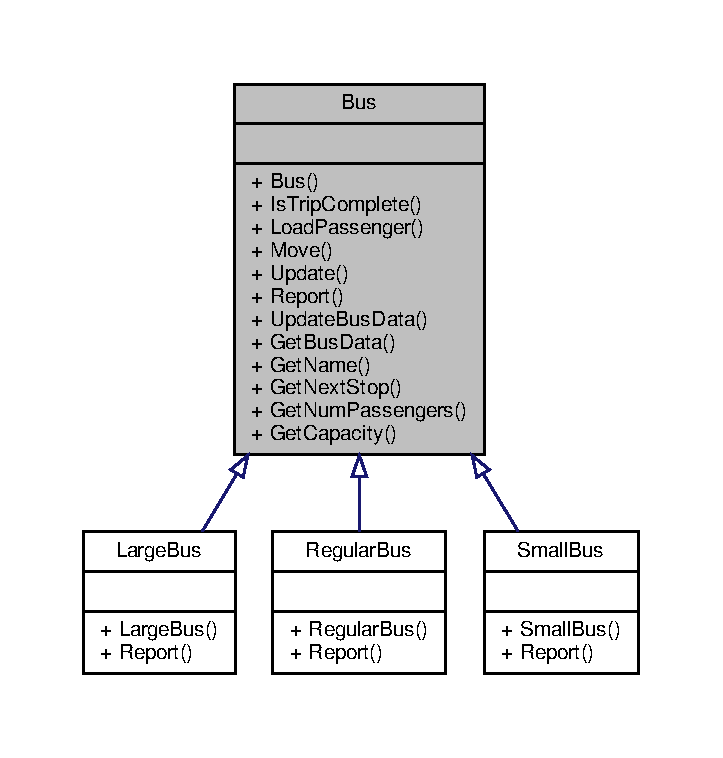
\includegraphics[width=347pt]{classBus__inherit__graph}
\end{center}
\end{figure}


Collaboration diagram for Bus\+:\nopagebreak
\begin{figure}[H]
\begin{center}
\leavevmode
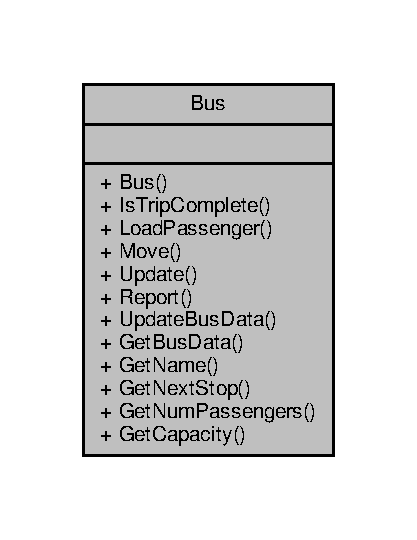
\includegraphics[width=200pt]{classBus__coll__graph}
\end{center}
\end{figure}
\subsection*{Public Member Functions}
\begin{DoxyCompactItemize}
\item 
\hyperlink{classBus_aa28c3c318b6993f3a3aebf211daa9217}{Bus} (std\+::string name, \hyperlink{classRoute}{Route} $\ast$out, \hyperlink{classRoute}{Route} $\ast$in, int capacity=60, double speed=1)
\begin{DoxyCompactList}\small\item\em is contructor that initialises \hyperlink{classBus}{Bus} object automatically when it is created. \end{DoxyCompactList}\item 
bool \hyperlink{classBus_a9c64b0801bf589f121fb0598b70a99b4}{Is\+Trip\+Complete} ()
\begin{DoxyCompactList}\small\item\em represent if the bus reach the end of route. \end{DoxyCompactList}\item 
bool \hyperlink{classBus_ac3f1c523bc4f97bc8ada8dc488ab3484}{Load\+Passenger} (\hyperlink{classPassenger}{Passenger} $\ast$)
\begin{DoxyCompactList}\small\item\em represent add passenger in stops to the bus object \end{DoxyCompactList}\item 
bool \hyperlink{classBus_a5e667186d6db0916ebab0e4eff3312c8}{Move} ()
\begin{DoxyCompactList}\small\item\em represent the movement of every bue \end{DoxyCompactList}\item 
void \hyperlink{classBus_a9896f74f16966f7621d0dfafff0ec6b4}{Update} ()
\begin{DoxyCompactList}\small\item\em keep track each status that \hyperlink{classBus}{Bus} class process \end{DoxyCompactList}\item 
void \hyperlink{classBus_a4e50209dde52bff3de231c8259b38982}{Report} (std\+::ostream \&)
\begin{DoxyCompactList}\small\item\em display each status information to the screen \end{DoxyCompactList}\item 
void \hyperlink{classBus_a38b7ee7b13b3438894e914a6933a6f44}{Update\+Bus\+Data} ()
\begin{DoxyCompactList}\small\item\em represent update each status of \hyperlink{classBus}{Bus} object \end{DoxyCompactList}\item 
\hyperlink{structBusData}{Bus\+Data} \hyperlink{classBus_aee8d077fc426b73942dec2564b5d066a}{Get\+Bus\+Data} () const
\begin{DoxyCompactList}\small\item\em obtain the bus data from Vis \end{DoxyCompactList}\item 
std\+::string \hyperlink{classBus_a2143b0563ad48b1b67e114d1ba5342ca}{Get\+Name} () const
\begin{DoxyCompactList}\small\item\em obtain the bus id \end{DoxyCompactList}\item 
\hyperlink{classStop}{Stop} $\ast$ \hyperlink{classBus_a6068e9801c6da152f05e40eb26e80b02}{Get\+Next\+Stop} () const
\begin{DoxyCompactList}\small\item\em obtain the stop data from Vis \end{DoxyCompactList}\item 
size\+\_\+t \hyperlink{classBus_a346aaa56030d4707886e1db8181e8b55}{Get\+Num\+Passengers} () const
\begin{DoxyCompactList}\small\item\em obtain the number of passenger on bus \end{DoxyCompactList}\item 
int \hyperlink{classBus_a3a1f68e9e2548f981d0150901918922c}{Get\+Capacity} () const
\begin{DoxyCompactList}\small\item\em obtain the max capacity of bus \end{DoxyCompactList}\end{DoxyCompactItemize}


\subsection{Detailed Description}
The main class for the bus. 

Calls to Generate function to get a new instance of a bus. This is a static call, not requiring an instance to invoke the method. 

\subsection{Constructor \& Destructor Documentation}
\mbox{\Hypertarget{classBus_aa28c3c318b6993f3a3aebf211daa9217}\label{classBus_aa28c3c318b6993f3a3aebf211daa9217}} 
\index{Bus@{Bus}!Bus@{Bus}}
\index{Bus@{Bus}!Bus@{Bus}}
\subsubsection{\texorpdfstring{Bus()}{Bus()}}
{\footnotesize\ttfamily Bus\+::\+Bus (\begin{DoxyParamCaption}\item[{std\+::string}]{name,  }\item[{\hyperlink{classRoute}{Route} $\ast$}]{out,  }\item[{\hyperlink{classRoute}{Route} $\ast$}]{in,  }\item[{int}]{capacity = {\ttfamily 60},  }\item[{double}]{speed = {\ttfamily 1} }\end{DoxyParamCaption})}



is contructor that initialises \hyperlink{classBus}{Bus} object automatically when it is created. 

This function will be used for simulation purposes.


\begin{DoxyParams}[1]{Parameters}
\mbox{\tt in}  & {\em name} & bus id, left bound (not-\/inclusive) \\
\hline
\mbox{\tt in}  & {\em out} & outgoing route, right bound (inclusive) \\
\hline
\mbox{\tt in}  & {\em in} & incoming route, left bound (not-\/inclusive) \\
\hline
\mbox{\tt in}  & {\em capacity} & capacity of bus, right bound (inclusive) \\
\hline
\mbox{\tt in}  & {\em speed} & Speed of bus, left bound (not-\/inclusive) \\
\hline
\end{DoxyParams}


\subsection{Member Function Documentation}
\mbox{\Hypertarget{classBus_aee8d077fc426b73942dec2564b5d066a}\label{classBus_aee8d077fc426b73942dec2564b5d066a}} 
\index{Bus@{Bus}!Get\+Bus\+Data@{Get\+Bus\+Data}}
\index{Get\+Bus\+Data@{Get\+Bus\+Data}!Bus@{Bus}}
\subsubsection{\texorpdfstring{Get\+Bus\+Data()}{GetBusData()}}
{\footnotesize\ttfamily \hyperlink{structBusData}{Bus\+Data} Bus\+::\+Get\+Bus\+Data (\begin{DoxyParamCaption}{ }\end{DoxyParamCaption}) const}



obtain the bus data from Vis 

This function will be used for simulation purposes.

\begin{DoxyReturn}{Returns}
bus\+\_\+data\+\_\+ \hyperlink{classBus}{Bus} Data. 
\end{DoxyReturn}
\mbox{\Hypertarget{classBus_a3a1f68e9e2548f981d0150901918922c}\label{classBus_a3a1f68e9e2548f981d0150901918922c}} 
\index{Bus@{Bus}!Get\+Capacity@{Get\+Capacity}}
\index{Get\+Capacity@{Get\+Capacity}!Bus@{Bus}}
\subsubsection{\texorpdfstring{Get\+Capacity()}{GetCapacity()}}
{\footnotesize\ttfamily int Bus\+::\+Get\+Capacity (\begin{DoxyParamCaption}{ }\end{DoxyParamCaption}) const\hspace{0.3cm}{\ttfamily [inline]}}



obtain the max capacity of bus 

This function will be used for simulation purposes.

\begin{DoxyReturn}{Returns}
passenger\+\_\+max\+\_\+capacity\+\_\+ \hyperlink{classPassenger}{Passenger} Max Capacity. 
\end{DoxyReturn}
\mbox{\Hypertarget{classBus_a2143b0563ad48b1b67e114d1ba5342ca}\label{classBus_a2143b0563ad48b1b67e114d1ba5342ca}} 
\index{Bus@{Bus}!Get\+Name@{Get\+Name}}
\index{Get\+Name@{Get\+Name}!Bus@{Bus}}
\subsubsection{\texorpdfstring{Get\+Name()}{GetName()}}
{\footnotesize\ttfamily std\+::string Bus\+::\+Get\+Name (\begin{DoxyParamCaption}{ }\end{DoxyParamCaption}) const\hspace{0.3cm}{\ttfamily [inline]}}



obtain the bus id 

This function will be used for simulation purposes.

\begin{DoxyReturn}{Returns}
name\+\_\+ \hyperlink{classBus}{Bus} id. 
\end{DoxyReturn}
\mbox{\Hypertarget{classBus_a6068e9801c6da152f05e40eb26e80b02}\label{classBus_a6068e9801c6da152f05e40eb26e80b02}} 
\index{Bus@{Bus}!Get\+Next\+Stop@{Get\+Next\+Stop}}
\index{Get\+Next\+Stop@{Get\+Next\+Stop}!Bus@{Bus}}
\subsubsection{\texorpdfstring{Get\+Next\+Stop()}{GetNextStop()}}
{\footnotesize\ttfamily \hyperlink{classStop}{Stop}$\ast$ Bus\+::\+Get\+Next\+Stop (\begin{DoxyParamCaption}{ }\end{DoxyParamCaption}) const\hspace{0.3cm}{\ttfamily [inline]}}



obtain the stop data from Vis 

This function will be used for simulation purposes.

\begin{DoxyReturn}{Returns}
next\+\_\+stop\+\_\+ Next \hyperlink{classStop}{Stop}. 
\end{DoxyReturn}
\mbox{\Hypertarget{classBus_a346aaa56030d4707886e1db8181e8b55}\label{classBus_a346aaa56030d4707886e1db8181e8b55}} 
\index{Bus@{Bus}!Get\+Num\+Passengers@{Get\+Num\+Passengers}}
\index{Get\+Num\+Passengers@{Get\+Num\+Passengers}!Bus@{Bus}}
\subsubsection{\texorpdfstring{Get\+Num\+Passengers()}{GetNumPassengers()}}
{\footnotesize\ttfamily size\+\_\+t Bus\+::\+Get\+Num\+Passengers (\begin{DoxyParamCaption}{ }\end{DoxyParamCaption}) const\hspace{0.3cm}{\ttfamily [inline]}}



obtain the number of passenger on bus 

This function will be used for simulation purposes.

\begin{DoxyReturn}{Returns}
passengers\+\_\+.\+size() count length of list which represent number of passenger. 
\end{DoxyReturn}
\mbox{\Hypertarget{classBus_a9c64b0801bf589f121fb0598b70a99b4}\label{classBus_a9c64b0801bf589f121fb0598b70a99b4}} 
\index{Bus@{Bus}!Is\+Trip\+Complete@{Is\+Trip\+Complete}}
\index{Is\+Trip\+Complete@{Is\+Trip\+Complete}!Bus@{Bus}}
\subsubsection{\texorpdfstring{Is\+Trip\+Complete()}{IsTripComplete()}}
{\footnotesize\ttfamily bool Bus\+::\+Is\+Trip\+Complete (\begin{DoxyParamCaption}{ }\end{DoxyParamCaption})}



represent if the bus reach the end of route. 

This function will be used for simulation purposes.

\begin{DoxyReturn}{Returns}
true if bus reach the end, else return false 
\end{DoxyReturn}
\mbox{\Hypertarget{classBus_ac3f1c523bc4f97bc8ada8dc488ab3484}\label{classBus_ac3f1c523bc4f97bc8ada8dc488ab3484}} 
\index{Bus@{Bus}!Load\+Passenger@{Load\+Passenger}}
\index{Load\+Passenger@{Load\+Passenger}!Bus@{Bus}}
\subsubsection{\texorpdfstring{Load\+Passenger()}{LoadPassenger()}}
{\footnotesize\ttfamily bool Bus\+::\+Load\+Passenger (\begin{DoxyParamCaption}\item[{\hyperlink{classPassenger}{Passenger} $\ast$}]{new\+\_\+passenger }\end{DoxyParamCaption})}



represent add passenger in stops to the bus object 

This function will be used for simulation purposes.


\begin{DoxyParams}[1]{Parameters}
\mbox{\tt in}  & {\em new\+\_\+passenger} & New \hyperlink{classPassenger}{Passenger}, left bound (not-\/inclusive)\\
\hline
\end{DoxyParams}
\begin{DoxyReturn}{Returns}
true if load passenge, else retrun false. 
\end{DoxyReturn}
\mbox{\Hypertarget{classBus_a5e667186d6db0916ebab0e4eff3312c8}\label{classBus_a5e667186d6db0916ebab0e4eff3312c8}} 
\index{Bus@{Bus}!Move@{Move}}
\index{Move@{Move}!Bus@{Bus}}
\subsubsection{\texorpdfstring{Move()}{Move()}}
{\footnotesize\ttfamily bool Bus\+::\+Move (\begin{DoxyParamCaption}{ }\end{DoxyParamCaption})}



represent the movement of every bue 

This function will be used for simulation purposes.

\begin{DoxyReturn}{Returns}
true if the bus moved, else return false 
\end{DoxyReturn}
\mbox{\Hypertarget{classBus_a4e50209dde52bff3de231c8259b38982}\label{classBus_a4e50209dde52bff3de231c8259b38982}} 
\index{Bus@{Bus}!Report@{Report}}
\index{Report@{Report}!Bus@{Bus}}
\subsubsection{\texorpdfstring{Report()}{Report()}}
{\footnotesize\ttfamily void Bus\+::\+Report (\begin{DoxyParamCaption}\item[{std\+::ostream \&}]{out }\end{DoxyParamCaption})}



display each status information to the screen 


\begin{DoxyParams}[1]{Parameters}
\mbox{\tt in}  & {\em out} & Display Out, left bound (not-\/inclusive)\\
\hline
\end{DoxyParams}
This function will be used for simulation purposes. \mbox{\Hypertarget{classBus_a9896f74f16966f7621d0dfafff0ec6b4}\label{classBus_a9896f74f16966f7621d0dfafff0ec6b4}} 
\index{Bus@{Bus}!Update@{Update}}
\index{Update@{Update}!Bus@{Bus}}
\subsubsection{\texorpdfstring{Update()}{Update()}}
{\footnotesize\ttfamily void Bus\+::\+Update (\begin{DoxyParamCaption}{ }\end{DoxyParamCaption})}



keep track each status that \hyperlink{classBus}{Bus} class process 

This function will be used for simulation purposes. \mbox{\Hypertarget{classBus_a38b7ee7b13b3438894e914a6933a6f44}\label{classBus_a38b7ee7b13b3438894e914a6933a6f44}} 
\index{Bus@{Bus}!Update\+Bus\+Data@{Update\+Bus\+Data}}
\index{Update\+Bus\+Data@{Update\+Bus\+Data}!Bus@{Bus}}
\subsubsection{\texorpdfstring{Update\+Bus\+Data()}{UpdateBusData()}}
{\footnotesize\ttfamily void Bus\+::\+Update\+Bus\+Data (\begin{DoxyParamCaption}{ }\end{DoxyParamCaption})}



represent update each status of \hyperlink{classBus}{Bus} object 

This function will be used for simulation purposes. 

The documentation for this class was generated from the following files\+:\begin{DoxyCompactItemize}
\item 
/home/wang8635/3081\+\_\+s20/repo-\/wang8635/project/src/\hyperlink{bus_8h}{bus.\+h}\item 
/home/wang8635/3081\+\_\+s20/repo-\/wang8635/project/src/\hyperlink{bus_8cc}{bus.\+cc}\end{DoxyCompactItemize}

\hypertarget{structBusData}{}\section{Bus\+Data Struct Reference}
\label{structBusData}\index{Bus\+Data@{Bus\+Data}}


Collaboration diagram for Bus\+Data\+:\nopagebreak
\begin{figure}[H]
\begin{center}
\leavevmode
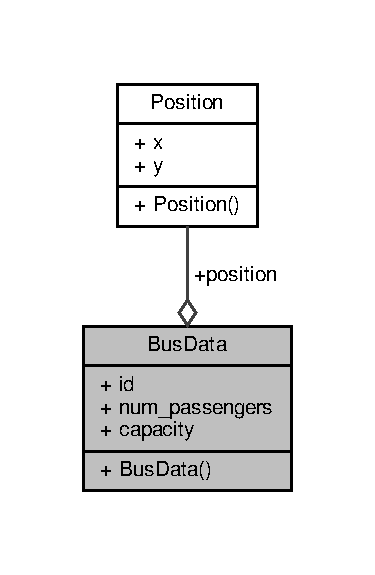
\includegraphics[width=180pt]{structBusData__coll__graph}
\end{center}
\end{figure}
\subsection*{Public Attributes}
\begin{DoxyCompactItemize}
\item 
\mbox{\Hypertarget{structBusData_aaae4f1be20f1ee54bb4dd773b8580069}\label{structBusData_aaae4f1be20f1ee54bb4dd773b8580069}} 
std\+::string {\bfseries id}
\item 
\mbox{\Hypertarget{structBusData_ae56b05c0d23a89ced4a0333bd65f0c96}\label{structBusData_ae56b05c0d23a89ced4a0333bd65f0c96}} 
\hyperlink{structPosition}{Position} {\bfseries position}
\item 
\mbox{\Hypertarget{structBusData_a4293fd5e2ffdcdd1b02a9e56f27230ec}\label{structBusData_a4293fd5e2ffdcdd1b02a9e56f27230ec}} 
int {\bfseries num\+\_\+passengers}
\item 
\mbox{\Hypertarget{structBusData_a84ea609f6ecc9b96e1ce37b47d2127a1}\label{structBusData_a84ea609f6ecc9b96e1ce37b47d2127a1}} 
int {\bfseries capacity}
\end{DoxyCompactItemize}


The documentation for this struct was generated from the following file\+:\begin{DoxyCompactItemize}
\item 
/home/wang8635/3081\+\_\+s20/repo-\/wang8635/project/src/data\+\_\+structs.\+h\end{DoxyCompactItemize}

\hypertarget{classBusFactory}{}\section{Bus\+Factory Class Reference}
\label{classBusFactory}\index{Bus\+Factory@{Bus\+Factory}}


The main class for the generation of bus.  




{\ttfamily \#include $<$bus\+\_\+factory.\+h$>$}



Collaboration diagram for Bus\+Factory\+:\nopagebreak
\begin{figure}[H]
\begin{center}
\leavevmode
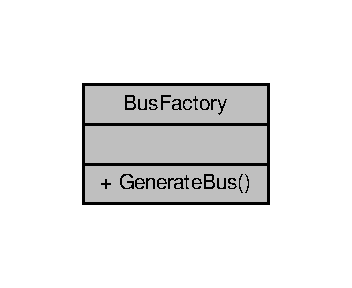
\includegraphics[width=169pt]{classBusFactory__coll__graph}
\end{center}
\end{figure}
\subsection*{Static Public Member Functions}
\begin{DoxyCompactItemize}
\item 
static \hyperlink{classBus}{Bus} $\ast$ \hyperlink{classBusFactory_aea064c9058b7c1592ae5c12ee409c747}{Generate\+Bus} (std\+::string name, \hyperlink{classRoute}{Route} $\ast$out, \hyperlink{classRoute}{Route} $\ast$in, int capacity, double speed)
\begin{DoxyCompactList}\small\item\em this class represent of bus factory which randomly generate 3 types of bus. \end{DoxyCompactList}\end{DoxyCompactItemize}


\subsection{Detailed Description}
The main class for the generation of bus. 

Calls to Generate function to get a new instance of a bus. This is a static call, not requiring an instance to invoke the method. 

\subsection{Member Function Documentation}
\mbox{\Hypertarget{classBusFactory_aea064c9058b7c1592ae5c12ee409c747}\label{classBusFactory_aea064c9058b7c1592ae5c12ee409c747}} 
\index{Bus\+Factory@{Bus\+Factory}!Generate\+Bus@{Generate\+Bus}}
\index{Generate\+Bus@{Generate\+Bus}!Bus\+Factory@{Bus\+Factory}}
\subsubsection{\texorpdfstring{Generate\+Bus()}{GenerateBus()}}
{\footnotesize\ttfamily \hyperlink{classBus}{Bus} $\ast$ Bus\+Factory\+::\+Generate\+Bus (\begin{DoxyParamCaption}\item[{std\+::string}]{name,  }\item[{\hyperlink{classRoute}{Route} $\ast$}]{out,  }\item[{\hyperlink{classRoute}{Route} $\ast$}]{in,  }\item[{int}]{capacity,  }\item[{double}]{speed }\end{DoxyParamCaption})\hspace{0.3cm}{\ttfamily [static]}}



this class represent of bus factory which randomly generate 3 types of bus. 

This function will be used for simulation purposes.


\begin{DoxyParams}[1]{Parameters}
\mbox{\tt in}  & {\em name} & bus id, left bound (not-\/inclusive) \\
\hline
\mbox{\tt in}  & {\em out} & outgoing route, right bound (inclusive) \\
\hline
\mbox{\tt in}  & {\em in} & incoming route, left bound (not-\/inclusive) \\
\hline
\mbox{\tt in}  & {\em capacity} & capacity of bus, right bound (inclusive) \\
\hline
\mbox{\tt in}  & {\em speed} & Speed of bus, left bound (not-\/inclusive)\\
\hline
\end{DoxyParams}
\begin{DoxyReturn}{Returns}
\hyperlink{classBus}{Bus} object with bus id, outgoing route, incoming route, capacity, speed. 
\end{DoxyReturn}


The documentation for this class was generated from the following files\+:\begin{DoxyCompactItemize}
\item 
/home/wang8635/3081\+\_\+s20/repo-\/wang8635/project/src/\hyperlink{bus__factory_8h}{bus\+\_\+factory.\+h}\item 
/home/wang8635/3081\+\_\+s20/repo-\/wang8635/project/src/\hyperlink{bus__factory_8cc}{bus\+\_\+factory.\+cc}\end{DoxyCompactItemize}

\hypertarget{classConfigManager}{}\section{Config\+Manager Class Reference}
\label{classConfigManager}\index{Config\+Manager@{Config\+Manager}}


Collaboration diagram for Config\+Manager\+:
\nopagebreak
\begin{figure}[H]
\begin{center}
\leavevmode
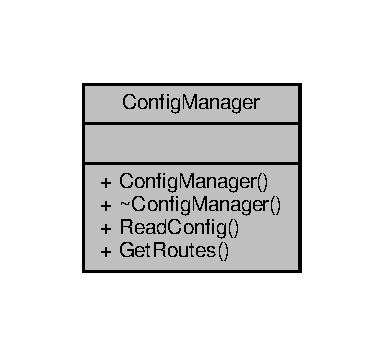
\includegraphics[width=184pt]{classConfigManager__coll__graph}
\end{center}
\end{figure}
\subsection*{Public Member Functions}
\begin{DoxyCompactItemize}
\item 
\hyperlink{classConfigManager_a7d3d7c10423d969f7544509f6fcca32f}{Config\+Manager} ()
\begin{DoxyCompactList}\small\item\em is contructor that initialises \hyperlink{classBus}{Bus} object automatically when it is created. \end{DoxyCompactList}\item 
\hyperlink{classConfigManager_a7fa65fdff98bdd5bbbf72196bd9ccf17}{$\sim$\+Config\+Manager} ()
\begin{DoxyCompactList}\small\item\em is copy contructor that initialises route data automatically when it is created. \end{DoxyCompactList}\item 
void \hyperlink{classConfigManager_ab8087a9f44ddaa001ea361b56514e64a}{Read\+Config} (const std\+::string filename)
\begin{DoxyCompactList}\small\item\em read config.\+text file content \end{DoxyCompactList}\item 
std\+::vector$<$ \hyperlink{classRoute}{Route} $\ast$ $>$ \hyperlink{classConfigManager_a0db6329b7dd5ac1f92ee262c30df4ef9}{Get\+Routes} () const
\begin{DoxyCompactList}\small\item\em Generatre \hyperlink{classRoute}{Route} object. \end{DoxyCompactList}\end{DoxyCompactItemize}


\subsection{Constructor \& Destructor Documentation}
\mbox{\Hypertarget{classConfigManager_a7d3d7c10423d969f7544509f6fcca32f}\label{classConfigManager_a7d3d7c10423d969f7544509f6fcca32f}} 
\index{Config\+Manager@{Config\+Manager}!Config\+Manager@{Config\+Manager}}
\index{Config\+Manager@{Config\+Manager}!Config\+Manager@{Config\+Manager}}
\subsubsection{\texorpdfstring{Config\+Manager()}{ConfigManager()}}
{\footnotesize\ttfamily Config\+Manager\+::\+Config\+Manager (\begin{DoxyParamCaption}{ }\end{DoxyParamCaption})}



is contructor that initialises \hyperlink{classBus}{Bus} object automatically when it is created. 

This function will be used for simulation purposes. \mbox{\Hypertarget{classConfigManager_a7fa65fdff98bdd5bbbf72196bd9ccf17}\label{classConfigManager_a7fa65fdff98bdd5bbbf72196bd9ccf17}} 
\index{Config\+Manager@{Config\+Manager}!````~Config\+Manager@{$\sim$\+Config\+Manager}}
\index{````~Config\+Manager@{$\sim$\+Config\+Manager}!Config\+Manager@{Config\+Manager}}
\subsubsection{\texorpdfstring{$\sim$\+Config\+Manager()}{~ConfigManager()}}
{\footnotesize\ttfamily Config\+Manager\+::$\sim$\+Config\+Manager (\begin{DoxyParamCaption}{ }\end{DoxyParamCaption})}



is copy contructor that initialises route data automatically when it is created. 

This function will be used for simulation purposes. 

\subsection{Member Function Documentation}
\mbox{\Hypertarget{classConfigManager_a0db6329b7dd5ac1f92ee262c30df4ef9}\label{classConfigManager_a0db6329b7dd5ac1f92ee262c30df4ef9}} 
\index{Config\+Manager@{Config\+Manager}!Get\+Routes@{Get\+Routes}}
\index{Get\+Routes@{Get\+Routes}!Config\+Manager@{Config\+Manager}}
\subsubsection{\texorpdfstring{Get\+Routes()}{GetRoutes()}}
{\footnotesize\ttfamily std\+::vector$<$\hyperlink{classRoute}{Route} $\ast$$>$ Config\+Manager\+::\+Get\+Routes (\begin{DoxyParamCaption}{ }\end{DoxyParamCaption}) const\hspace{0.3cm}{\ttfamily [inline]}}



Generatre \hyperlink{classRoute}{Route} object. 

This function will be used for simulation purposes.

\begin{DoxyReturn}{Returns}
route object. 
\end{DoxyReturn}
\mbox{\Hypertarget{classConfigManager_ab8087a9f44ddaa001ea361b56514e64a}\label{classConfigManager_ab8087a9f44ddaa001ea361b56514e64a}} 
\index{Config\+Manager@{Config\+Manager}!Read\+Config@{Read\+Config}}
\index{Read\+Config@{Read\+Config}!Config\+Manager@{Config\+Manager}}
\subsubsection{\texorpdfstring{Read\+Config()}{ReadConfig()}}
{\footnotesize\ttfamily void Config\+Manager\+::\+Read\+Config (\begin{DoxyParamCaption}\item[{const std\+::string}]{filename }\end{DoxyParamCaption})}



read config.\+text file content 

This function will be used for simulation purposes.


\begin{DoxyParams}[1]{Parameters}
\mbox{\tt in}  & {\em filename} & File Path, left bound (not-\/inclusive)\\
\hline
\end{DoxyParams}
\begin{DoxyReturn}{Returns}
\hyperlink{classPassenger}{Passenger} object with name and destination. 
\end{DoxyReturn}


The documentation for this class was generated from the following files\+:\begin{DoxyCompactItemize}
\item 
/home/wang8635/3081\+\_\+s20/repo-\/wang8635/project/src/config\+\_\+manager.\+h\item 
/home/wang8635/3081\+\_\+s20/repo-\/wang8635/project/src/config\+\_\+manager.\+cc\end{DoxyCompactItemize}

\hypertarget{classLargeBus}{}\section{Large\+Bus Class Reference}
\label{classLargeBus}\index{Large\+Bus@{Large\+Bus}}


The main class for the generation of regular bus.  




{\ttfamily \#include $<$large\+\_\+bus.\+h$>$}



Inheritance diagram for Large\+Bus\+:\nopagebreak
\begin{figure}[H]
\begin{center}
\leavevmode
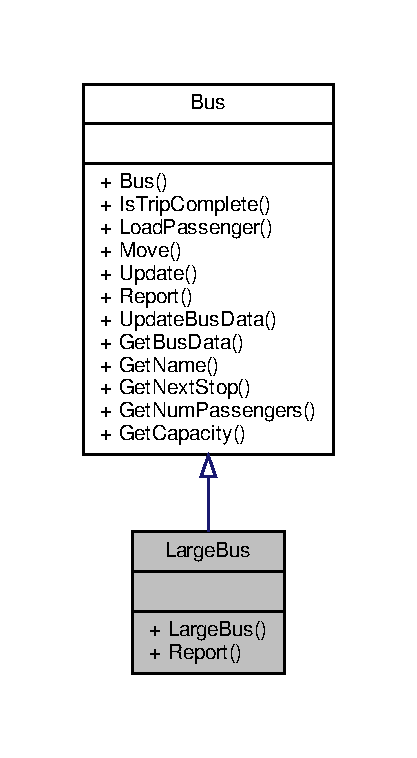
\includegraphics[width=200pt]{classLargeBus__inherit__graph}
\end{center}
\end{figure}


Collaboration diagram for Large\+Bus\+:\nopagebreak
\begin{figure}[H]
\begin{center}
\leavevmode
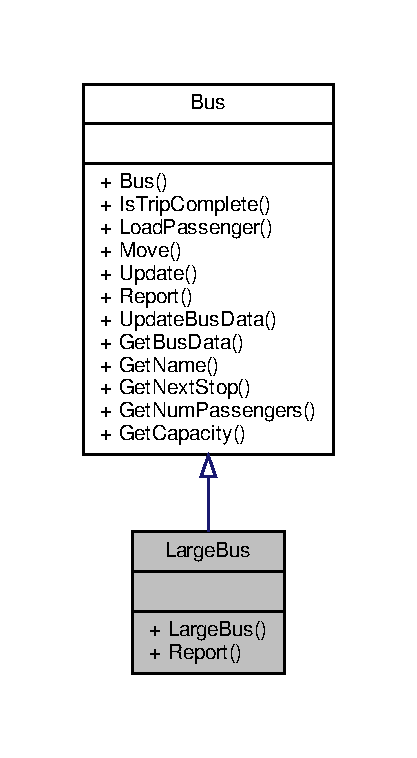
\includegraphics[width=200pt]{classLargeBus__coll__graph}
\end{center}
\end{figure}
\subsection*{Public Member Functions}
\begin{DoxyCompactItemize}
\item 
\hyperlink{classLargeBus_a17f3647b231039dbc42b006e51a43aa9}{Large\+Bus} (std\+::string name, \hyperlink{classRoute}{Route} $\ast$out, \hyperlink{classRoute}{Route} $\ast$in, int capacity, double speed)
\begin{DoxyCompactList}\small\item\em this class represent of generateor which randomly generate regular bus. \end{DoxyCompactList}\item 
void \hyperlink{classLargeBus_a401d909a31f2adf60b2f92681a2541d0}{Report} (std\+::ostream \&)
\begin{DoxyCompactList}\small\item\em this class represent of generate 3 number that relate to 3 different buses. \end{DoxyCompactList}\end{DoxyCompactItemize}


\subsection{Detailed Description}
The main class for the generation of regular bus. 

Calls to Generate function to get a new instance of a bus. This is a static call, not requiring an instance to invoke the method. 

\subsection{Constructor \& Destructor Documentation}
\mbox{\Hypertarget{classLargeBus_a17f3647b231039dbc42b006e51a43aa9}\label{classLargeBus_a17f3647b231039dbc42b006e51a43aa9}} 
\index{Large\+Bus@{Large\+Bus}!Large\+Bus@{Large\+Bus}}
\index{Large\+Bus@{Large\+Bus}!Large\+Bus@{Large\+Bus}}
\subsubsection{\texorpdfstring{Large\+Bus()}{LargeBus()}}
{\footnotesize\ttfamily Large\+Bus\+::\+Large\+Bus (\begin{DoxyParamCaption}\item[{std\+::string}]{name,  }\item[{\hyperlink{classRoute}{Route} $\ast$}]{out,  }\item[{\hyperlink{classRoute}{Route} $\ast$}]{in,  }\item[{int}]{capacity,  }\item[{double}]{speed }\end{DoxyParamCaption})}



this class represent of generateor which randomly generate regular bus. 

This function will be used for simulation purposes.


\begin{DoxyParams}[1]{Parameters}
\mbox{\tt in}  & {\em name} & bus id, left bound (not-\/inclusive) \\
\hline
\mbox{\tt in}  & {\em out} & outgoing route, right bound (inclusive) \\
\hline
\mbox{\tt in}  & {\em in} & incoming route, left bound (not-\/inclusive) \\
\hline
\mbox{\tt in}  & {\em capacity} & capacity of bus, right bound (inclusive) \\
\hline
\mbox{\tt in}  & {\em speed} & Speed of bus, left bound (not-\/inclusive)\\
\hline
\end{DoxyParams}
\begin{DoxyReturn}{Returns}
\hyperlink{classBus}{Bus} object with bus id, outgoing route, incoming route, regular capacity, speed. 
\end{DoxyReturn}


\subsection{Member Function Documentation}
\mbox{\Hypertarget{classLargeBus_a401d909a31f2adf60b2f92681a2541d0}\label{classLargeBus_a401d909a31f2adf60b2f92681a2541d0}} 
\index{Large\+Bus@{Large\+Bus}!Report@{Report}}
\index{Report@{Report}!Large\+Bus@{Large\+Bus}}
\subsubsection{\texorpdfstring{Report()}{Report()}}
{\footnotesize\ttfamily void Large\+Bus\+::\+Report (\begin{DoxyParamCaption}\item[{std\+::ostream \&}]{out }\end{DoxyParamCaption})}



this class represent of generate 3 number that relate to 3 different buses. 


\begin{DoxyParams}[1]{Parameters}
\mbox{\tt in}  & {\em std\+::ostream\&,left} & bound (not-\/inclusive)\\
\hline
\end{DoxyParams}
\begin{DoxyReturn}{Returns}
output bus detail. 
\end{DoxyReturn}


The documentation for this class was generated from the following files\+:\begin{DoxyCompactItemize}
\item 
/home/wang8635/3081\+\_\+s20/repo-\/wang8635/project/src/large\+\_\+bus.\+h\item 
/home/wang8635/3081\+\_\+s20/repo-\/wang8635/project/src/large\+\_\+bus.\+cc\end{DoxyCompactItemize}

\hypertarget{classPassenger}{}\section{Passenger Class Reference}
\label{classPassenger}\index{Passenger@{Passenger}}


Collaboration diagram for Passenger\+:\nopagebreak
\begin{figure}[H]
\begin{center}
\leavevmode
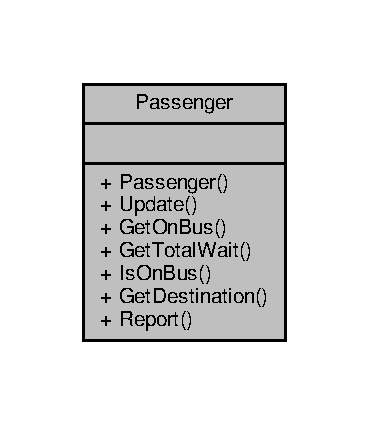
\includegraphics[width=177pt]{classPassenger__coll__graph}
\end{center}
\end{figure}
\subsection*{Public Member Functions}
\begin{DoxyCompactItemize}
\item 
\mbox{\Hypertarget{classPassenger_a5c3addb9a6fd03e5e5642ed844e2702c}\label{classPassenger_a5c3addb9a6fd03e5e5642ed844e2702c}} 
{\bfseries Passenger} (int=-\/1, std\+::string=\char`\"{}Nobody\char`\"{})
\item 
\mbox{\Hypertarget{classPassenger_a960de3b29fc17a2c2d79c0b79d5cf299}\label{classPassenger_a960de3b29fc17a2c2d79c0b79d5cf299}} 
void {\bfseries Update} ()
\item 
\mbox{\Hypertarget{classPassenger_ae2ba639cfef39781ac079778578bd9fe}\label{classPassenger_ae2ba639cfef39781ac079778578bd9fe}} 
void {\bfseries Get\+On\+Bus} ()
\item 
\mbox{\Hypertarget{classPassenger_a25158560f790ef7ef06d94c414b34f25}\label{classPassenger_a25158560f790ef7ef06d94c414b34f25}} 
int {\bfseries Get\+Total\+Wait} () const
\item 
\mbox{\Hypertarget{classPassenger_a2acf008ec444afcc859b914ee24add0e}\label{classPassenger_a2acf008ec444afcc859b914ee24add0e}} 
bool {\bfseries Is\+On\+Bus} () const
\item 
\mbox{\Hypertarget{classPassenger_a49db0ee527377aae6077df190a11501c}\label{classPassenger_a49db0ee527377aae6077df190a11501c}} 
int {\bfseries Get\+Destination} () const
\item 
\mbox{\Hypertarget{classPassenger_aee3f9d7f6f2a848034971559faf65248}\label{classPassenger_aee3f9d7f6f2a848034971559faf65248}} 
void {\bfseries Report} (std\+::ostream \&) const
\end{DoxyCompactItemize}


The documentation for this class was generated from the following files\+:\begin{DoxyCompactItemize}
\item 
/home/wang8635/3081\+\_\+s20/repo-\/wang8635/project/src/\hyperlink{passenger_8h}{passenger.\+h}\item 
/home/wang8635/3081\+\_\+s20/repo-\/wang8635/project/src/\hyperlink{passenger_8cc}{passenger.\+cc}\end{DoxyCompactItemize}

\hypertarget{classPassengerFactory}{}\section{Passenger\+Factory Class Reference}
\label{classPassengerFactory}\index{Passenger\+Factory@{Passenger\+Factory}}


Collaboration diagram for Passenger\+Factory\+:\nopagebreak
\begin{figure}[H]
\begin{center}
\leavevmode
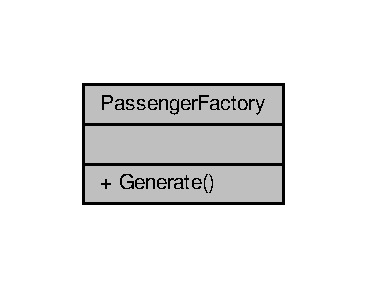
\includegraphics[width=176pt]{classPassengerFactory__coll__graph}
\end{center}
\end{figure}
\subsection*{Static Public Member Functions}
\begin{DoxyCompactItemize}
\item 
\mbox{\Hypertarget{classPassengerFactory_a2952ba78ceb285f445bc768d287230d2}\label{classPassengerFactory_a2952ba78ceb285f445bc768d287230d2}} 
static \hyperlink{classPassenger}{Passenger} $\ast$ {\bfseries Generate} (int, int)
\end{DoxyCompactItemize}


The documentation for this class was generated from the following files\+:\begin{DoxyCompactItemize}
\item 
/home/wang8635/3081\+\_\+s20/repo-\/wang8635/project/src/\hyperlink{passenger__factory_8h}{passenger\+\_\+factory.\+h}\item 
/home/wang8635/3081\+\_\+s20/repo-\/wang8635/project/src/\hyperlink{passenger__factory_8cc}{passenger\+\_\+factory.\+cc}\end{DoxyCompactItemize}

\hypertarget{classPassengerGenerator}{}\section{Passenger\+Generator Class Reference}
\label{classPassengerGenerator}\index{Passenger\+Generator@{Passenger\+Generator}}


Inheritance diagram for Passenger\+Generator\+:
\nopagebreak
\begin{figure}[H]
\begin{center}
\leavevmode
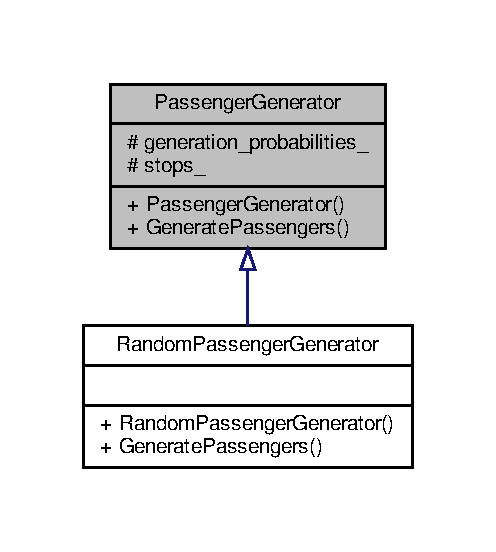
\includegraphics[width=238pt]{classPassengerGenerator__inherit__graph}
\end{center}
\end{figure}


Collaboration diagram for Passenger\+Generator\+:
\nopagebreak
\begin{figure}[H]
\begin{center}
\leavevmode
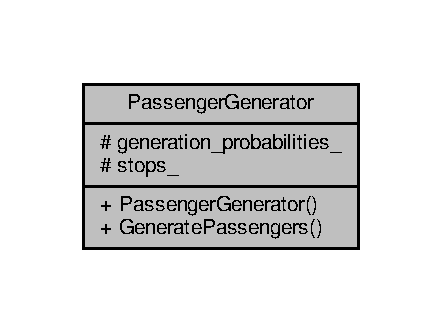
\includegraphics[width=212pt]{classPassengerGenerator__coll__graph}
\end{center}
\end{figure}
\subsection*{Public Member Functions}
\begin{DoxyCompactItemize}
\item 
\mbox{\Hypertarget{classPassengerGenerator_a33eeed8b68d5d596ceef5381c697e49d}\label{classPassengerGenerator_a33eeed8b68d5d596ceef5381c697e49d}} 
{\bfseries Passenger\+Generator} (std\+::list$<$ double $>$, std\+::list$<$ \hyperlink{classStop}{Stop} $\ast$$>$)
\item 
\mbox{\Hypertarget{classPassengerGenerator_ad2db96a13b34fcf35977287c06b31d47}\label{classPassengerGenerator_ad2db96a13b34fcf35977287c06b31d47}} 
virtual int {\bfseries Generate\+Passengers} ()=0
\end{DoxyCompactItemize}
\subsection*{Protected Attributes}
\begin{DoxyCompactItemize}
\item 
\mbox{\Hypertarget{classPassengerGenerator_a855471e5532fec3f387a6340f928d43a}\label{classPassengerGenerator_a855471e5532fec3f387a6340f928d43a}} 
std\+::list$<$ double $>$ {\bfseries generation\+\_\+probabilities\+\_\+}
\item 
\mbox{\Hypertarget{classPassengerGenerator_ab09ab7ca9104385ae007d05a6e957884}\label{classPassengerGenerator_ab09ab7ca9104385ae007d05a6e957884}} 
std\+::list$<$ \hyperlink{classStop}{Stop} $\ast$ $>$ {\bfseries stops\+\_\+}
\end{DoxyCompactItemize}


The documentation for this class was generated from the following files\+:\begin{DoxyCompactItemize}
\item 
/home/wang8635/3081\+\_\+s20/repo-\/wang8635/project/src/\hyperlink{passenger__generator_8h}{passenger\+\_\+generator.\+h}\item 
/home/wang8635/3081\+\_\+s20/repo-\/wang8635/project/src/\hyperlink{passenger__generator_8cc}{passenger\+\_\+generator.\+cc}\end{DoxyCompactItemize}

\hypertarget{classPassengerLoader}{}\section{Passenger\+Loader Class Reference}
\label{classPassengerLoader}\index{Passenger\+Loader@{Passenger\+Loader}}


Collaboration diagram for Passenger\+Loader\+:
\nopagebreak
\begin{figure}[H]
\begin{center}
\leavevmode
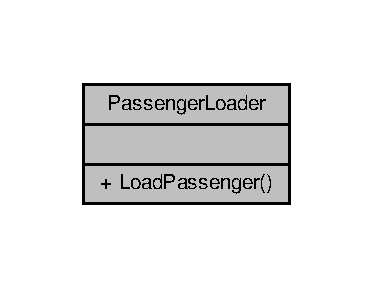
\includegraphics[width=179pt]{classPassengerLoader__coll__graph}
\end{center}
\end{figure}
\subsection*{Public Member Functions}
\begin{DoxyCompactItemize}
\item 
\mbox{\Hypertarget{classPassengerLoader_a804ae6e894dd35dd6984dfd3b9b06b34}\label{classPassengerLoader_a804ae6e894dd35dd6984dfd3b9b06b34}} 
int {\bfseries Load\+Passenger} (\hyperlink{classPassenger}{Passenger} $\ast$new\+\_\+passenger, int max\+\_\+pass, std\+::list$<$ \hyperlink{classPassenger}{Passenger} $\ast$$>$ $\ast$passengers)
\end{DoxyCompactItemize}


The documentation for this class was generated from the following files\+:\begin{DoxyCompactItemize}
\item 
/home/wang8635/3081\+\_\+s20/repo-\/wang8635/project/src/\hyperlink{passenger__loader_8h}{passenger\+\_\+loader.\+h}\item 
/home/wang8635/3081\+\_\+s20/repo-\/wang8635/project/src/\hyperlink{passenger__loader_8cc}{passenger\+\_\+loader.\+cc}\end{DoxyCompactItemize}

\hypertarget{classPassengerUnloader}{}\section{Passenger\+Unloader Class Reference}
\label{classPassengerUnloader}\index{Passenger\+Unloader@{Passenger\+Unloader}}


Collaboration diagram for Passenger\+Unloader\+:
\nopagebreak
\begin{figure}[H]
\begin{center}
\leavevmode
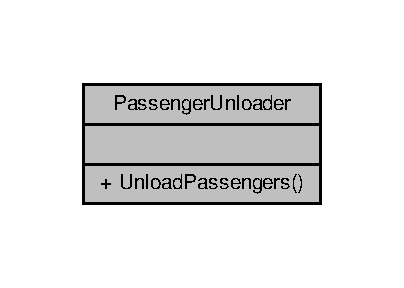
\includegraphics[width=194pt]{classPassengerUnloader__coll__graph}
\end{center}
\end{figure}
\subsection*{Public Member Functions}
\begin{DoxyCompactItemize}
\item 
\mbox{\Hypertarget{classPassengerUnloader_a571ee51523a6bce30fb843174eaad4a2}\label{classPassengerUnloader_a571ee51523a6bce30fb843174eaad4a2}} 
int {\bfseries Unload\+Passengers} (std\+::list$<$ \hyperlink{classPassenger}{Passenger} $\ast$$>$ $\ast$passengers, \hyperlink{classStop}{Stop} $\ast$current\+\_\+stop)
\end{DoxyCompactItemize}


The documentation for this class was generated from the following files\+:\begin{DoxyCompactItemize}
\item 
/home/wang8635/3081\+\_\+s20/repo-\/wang8635/project/src/\hyperlink{passenger__unloader_8h}{passenger\+\_\+unloader.\+h}\item 
/home/wang8635/3081\+\_\+s20/repo-\/wang8635/project/src/\hyperlink{passenger__unloader_8cc}{passenger\+\_\+unloader.\+cc}\end{DoxyCompactItemize}

\hypertarget{structPosition}{}\section{Position Struct Reference}
\label{structPosition}\index{Position@{Position}}


Collaboration diagram for Position\+:\nopagebreak
\begin{figure}[H]
\begin{center}
\leavevmode
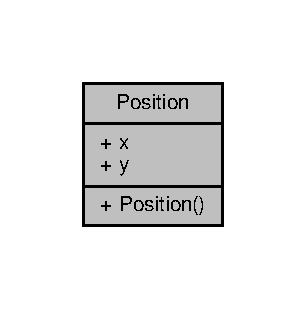
\includegraphics[width=147pt]{structPosition__coll__graph}
\end{center}
\end{figure}
\subsection*{Public Attributes}
\begin{DoxyCompactItemize}
\item 
\mbox{\Hypertarget{structPosition_af684446cbf0f6d53386686283da6dcc6}\label{structPosition_af684446cbf0f6d53386686283da6dcc6}} 
float {\bfseries x}
\item 
\mbox{\Hypertarget{structPosition_a54a6182b5f7539295b32255808897d3f}\label{structPosition_a54a6182b5f7539295b32255808897d3f}} 
float {\bfseries y}
\end{DoxyCompactItemize}


The documentation for this struct was generated from the following file\+:\begin{DoxyCompactItemize}
\item 
/home/wang8635/3081\+\_\+s20/repo-\/wang8635/project/src/data\+\_\+structs.\+h\end{DoxyCompactItemize}

\hypertarget{classRandomPassengerGenerator}{}\section{Random\+Passenger\+Generator Class Reference}
\label{classRandomPassengerGenerator}\index{Random\+Passenger\+Generator@{Random\+Passenger\+Generator}}


Inheritance diagram for Random\+Passenger\+Generator\+:\nopagebreak
\begin{figure}[H]
\begin{center}
\leavevmode
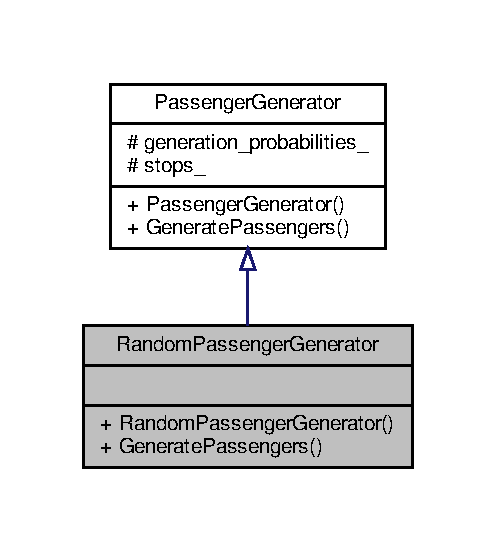
\includegraphics[width=238pt]{classRandomPassengerGenerator__inherit__graph}
\end{center}
\end{figure}


Collaboration diagram for Random\+Passenger\+Generator\+:\nopagebreak
\begin{figure}[H]
\begin{center}
\leavevmode
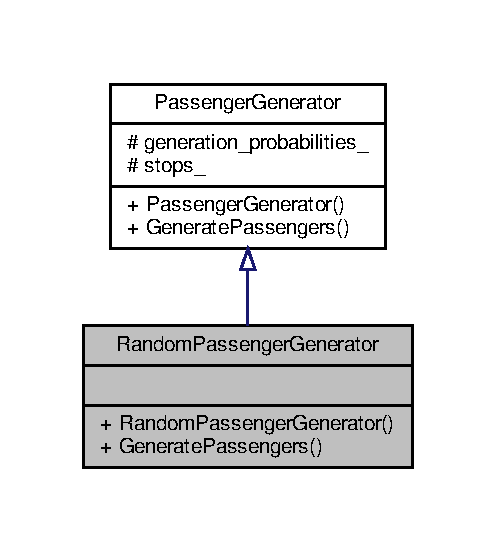
\includegraphics[width=238pt]{classRandomPassengerGenerator__coll__graph}
\end{center}
\end{figure}
\subsection*{Public Member Functions}
\begin{DoxyCompactItemize}
\item 
\mbox{\Hypertarget{classRandomPassengerGenerator_a1be1b4abfe82bfe95eb0a078d9a3342d}\label{classRandomPassengerGenerator_a1be1b4abfe82bfe95eb0a078d9a3342d}} 
{\bfseries Random\+Passenger\+Generator} (std\+::list$<$ double $>$, std\+::list$<$ \hyperlink{classStop}{Stop} $\ast$$>$)
\item 
\mbox{\Hypertarget{classRandomPassengerGenerator_aba2d80cde33371cf9c3d033f1b8ba6b8}\label{classRandomPassengerGenerator_aba2d80cde33371cf9c3d033f1b8ba6b8}} 
int {\bfseries Generate\+Passengers} () override
\end{DoxyCompactItemize}
\subsection*{Additional Inherited Members}


The documentation for this class was generated from the following files\+:\begin{DoxyCompactItemize}
\item 
/home/wang8635/3081\+\_\+s20/repo-\/wang8635/project/src/\hyperlink{random__passenger__generator_8h}{random\+\_\+passenger\+\_\+generator.\+h}\item 
/home/wang8635/3081\+\_\+s20/repo-\/wang8635/project/src/\hyperlink{random__passenger__generator_8cc}{random\+\_\+passenger\+\_\+generator.\+cc}\end{DoxyCompactItemize}

\hypertarget{classRegularBus}{}\section{Regular\+Bus Class Reference}
\label{classRegularBus}\index{Regular\+Bus@{Regular\+Bus}}


The main class for the generation of regular bus.  




{\ttfamily \#include $<$regular\+\_\+bus.\+h$>$}



Inheritance diagram for Regular\+Bus\+:
\nopagebreak
\begin{figure}[H]
\begin{center}
\leavevmode
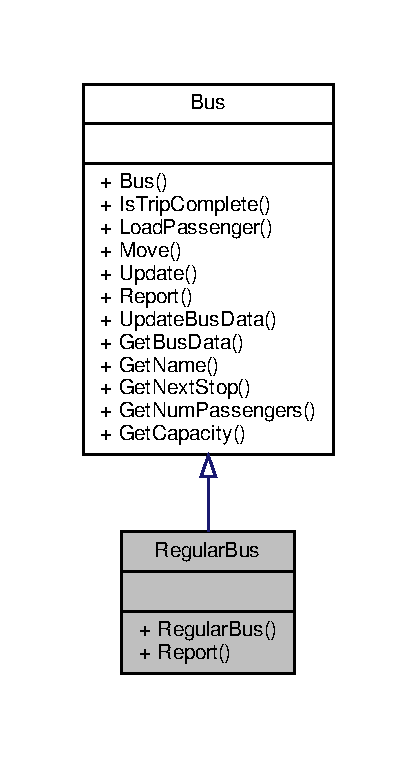
\includegraphics[width=200pt]{classRegularBus__inherit__graph}
\end{center}
\end{figure}


Collaboration diagram for Regular\+Bus\+:
\nopagebreak
\begin{figure}[H]
\begin{center}
\leavevmode
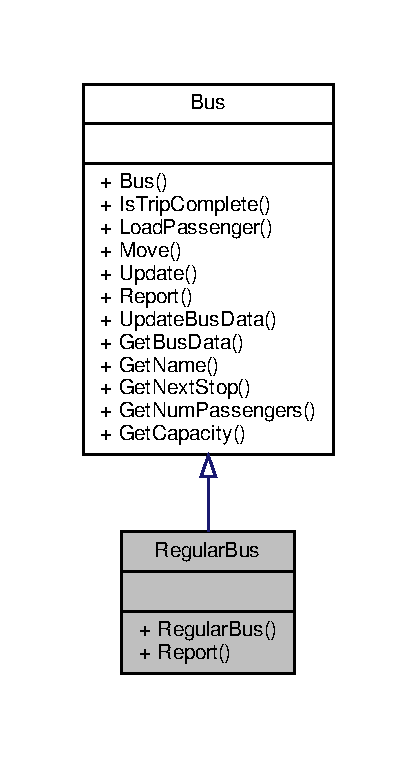
\includegraphics[width=200pt]{classRegularBus__coll__graph}
\end{center}
\end{figure}
\subsection*{Public Member Functions}
\begin{DoxyCompactItemize}
\item 
\hyperlink{classRegularBus_ac97f3951dee6538eb86d36ea0457947e}{Regular\+Bus} (std\+::string name, \hyperlink{classRoute}{Route} $\ast$out, \hyperlink{classRoute}{Route} $\ast$in, int capacity, double speed)
\begin{DoxyCompactList}\small\item\em this class represent of generateor which randomly generate regular bus. \end{DoxyCompactList}\item 
void \hyperlink{classRegularBus_a6ff6c67f22040ab2c9ad23649c3ba9dc}{Report} (std\+::ostream \&)
\begin{DoxyCompactList}\small\item\em this class represent of generate 3 number that relate to 3 different buses. \end{DoxyCompactList}\end{DoxyCompactItemize}


\subsection{Detailed Description}
The main class for the generation of regular bus. 

Calls to Generate function to get a new instance of a bus. This is a static call, not requiring an instance to invoke the method. 

\subsection{Constructor \& Destructor Documentation}
\mbox{\Hypertarget{classRegularBus_ac97f3951dee6538eb86d36ea0457947e}\label{classRegularBus_ac97f3951dee6538eb86d36ea0457947e}} 
\index{Regular\+Bus@{Regular\+Bus}!Regular\+Bus@{Regular\+Bus}}
\index{Regular\+Bus@{Regular\+Bus}!Regular\+Bus@{Regular\+Bus}}
\subsubsection{\texorpdfstring{Regular\+Bus()}{RegularBus()}}
{\footnotesize\ttfamily Regular\+Bus\+::\+Regular\+Bus (\begin{DoxyParamCaption}\item[{std\+::string}]{name,  }\item[{\hyperlink{classRoute}{Route} $\ast$}]{out,  }\item[{\hyperlink{classRoute}{Route} $\ast$}]{in,  }\item[{int}]{capacity,  }\item[{double}]{speed }\end{DoxyParamCaption})}



this class represent of generateor which randomly generate regular bus. 

This function will be used for simulation purposes.


\begin{DoxyParams}[1]{Parameters}
\mbox{\tt in}  & {\em name} & bus id, left bound (not-\/inclusive) \\
\hline
\mbox{\tt in}  & {\em out} & outgoing route, right bound (inclusive) \\
\hline
\mbox{\tt in}  & {\em in} & incoming route, left bound (not-\/inclusive) \\
\hline
\mbox{\tt in}  & {\em capacity} & capacity of bus, right bound (inclusive) \\
\hline
\mbox{\tt in}  & {\em speed} & Speed of bus, left bound (not-\/inclusive)\\
\hline
\end{DoxyParams}
\begin{DoxyReturn}{Returns}
\hyperlink{classBus}{Bus} object with bus id, outgoing route, incoming route, regular capacity, speed. 
\end{DoxyReturn}


\subsection{Member Function Documentation}
\mbox{\Hypertarget{classRegularBus_a6ff6c67f22040ab2c9ad23649c3ba9dc}\label{classRegularBus_a6ff6c67f22040ab2c9ad23649c3ba9dc}} 
\index{Regular\+Bus@{Regular\+Bus}!Report@{Report}}
\index{Report@{Report}!Regular\+Bus@{Regular\+Bus}}
\subsubsection{\texorpdfstring{Report()}{Report()}}
{\footnotesize\ttfamily void Regular\+Bus\+::\+Report (\begin{DoxyParamCaption}\item[{std\+::ostream \&}]{out }\end{DoxyParamCaption})}



this class represent of generate 3 number that relate to 3 different buses. 


\begin{DoxyParams}[1]{Parameters}
\mbox{\tt in}  & {\em std\+::ostream\&,left} & bound (not-\/inclusive)\\
\hline
\end{DoxyParams}
\begin{DoxyReturn}{Returns}
output bus detail. 
\end{DoxyReturn}


The documentation for this class was generated from the following files\+:\begin{DoxyCompactItemize}
\item 
/home/wang8635/3081\+\_\+s20/repo-\/wang8635/project/src/regular\+\_\+bus.\+h\item 
/home/wang8635/3081\+\_\+s20/repo-\/wang8635/project/src/regular\+\_\+bus.\+cc\end{DoxyCompactItemize}

\hypertarget{classRoute}{}\section{Route Class Reference}
\label{classRoute}\index{Route@{Route}}


Collaboration diagram for Route\+:
\nopagebreak
\begin{figure}[H]
\begin{center}
\leavevmode
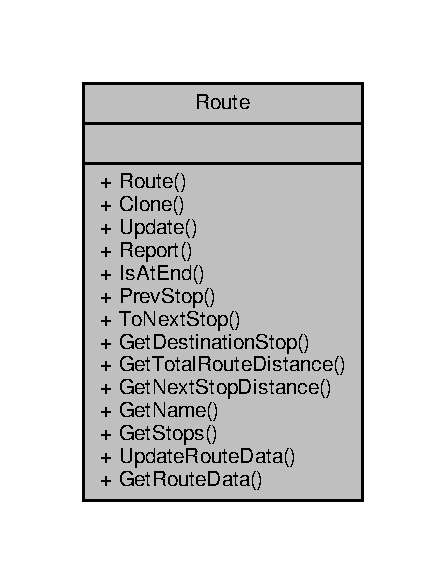
\includegraphics[width=214pt]{classRoute__coll__graph}
\end{center}
\end{figure}
\subsection*{Public Member Functions}
\begin{DoxyCompactItemize}
\item 
\mbox{\Hypertarget{classRoute_a623dad9165299b72eed1e188f7d3f382}\label{classRoute_a623dad9165299b72eed1e188f7d3f382}} 
{\bfseries Route} (std\+::string name, \hyperlink{classStop}{Stop} $\ast$$\ast$stops, double $\ast$distances, int num\+\_\+stops, \hyperlink{classPassengerGenerator}{Passenger\+Generator} $\ast$)
\item 
\mbox{\Hypertarget{classRoute_a4031b4a218b1530e28dcf5ee5c6fa8e7}\label{classRoute_a4031b4a218b1530e28dcf5ee5c6fa8e7}} 
\hyperlink{classRoute}{Route} $\ast$ {\bfseries Clone} ()
\item 
\mbox{\Hypertarget{classRoute_a7ecf1d4200f5fe110de4a1d9ea9408c3}\label{classRoute_a7ecf1d4200f5fe110de4a1d9ea9408c3}} 
void {\bfseries Update} ()
\item 
\mbox{\Hypertarget{classRoute_a6115a741ea15af716c1a624627ec954a}\label{classRoute_a6115a741ea15af716c1a624627ec954a}} 
void {\bfseries Report} (std\+::ostream \&)
\item 
\mbox{\Hypertarget{classRoute_a529ab995aefd1001b250a6c1ccf77892}\label{classRoute_a529ab995aefd1001b250a6c1ccf77892}} 
bool {\bfseries Is\+At\+End} () const
\item 
\mbox{\Hypertarget{classRoute_a1924b536cfdb17b5feea61e22fcb4a47}\label{classRoute_a1924b536cfdb17b5feea61e22fcb4a47}} 
\hyperlink{classStop}{Stop} $\ast$ {\bfseries Prev\+Stop} ()
\item 
\mbox{\Hypertarget{classRoute_a0d2be355c05f40fda3f0b4e1811d2583}\label{classRoute_a0d2be355c05f40fda3f0b4e1811d2583}} 
void {\bfseries To\+Next\+Stop} ()
\item 
\mbox{\Hypertarget{classRoute_a44af714485a55a8b6da374399e036cc1}\label{classRoute_a44af714485a55a8b6da374399e036cc1}} 
\hyperlink{classStop}{Stop} $\ast$ {\bfseries Get\+Destination\+Stop} () const
\item 
\mbox{\Hypertarget{classRoute_af4e0add4a9f6b22963398b41313f9e69}\label{classRoute_af4e0add4a9f6b22963398b41313f9e69}} 
double {\bfseries Get\+Total\+Route\+Distance} () const
\item 
\mbox{\Hypertarget{classRoute_af25192c44e2402660d54e7f32903ac25}\label{classRoute_af25192c44e2402660d54e7f32903ac25}} 
double {\bfseries Get\+Next\+Stop\+Distance} () const
\item 
\mbox{\Hypertarget{classRoute_a32bfa4fcc25a882be6ffd540c8723333}\label{classRoute_a32bfa4fcc25a882be6ffd540c8723333}} 
std\+::string {\bfseries Get\+Name} () const
\item 
\mbox{\Hypertarget{classRoute_afae0cf3fd696a06c9358d2d7152b7541}\label{classRoute_afae0cf3fd696a06c9358d2d7152b7541}} 
std\+::list$<$ \hyperlink{classStop}{Stop} $\ast$ $>$ {\bfseries Get\+Stops} () const
\item 
\mbox{\Hypertarget{classRoute_a0a8e0e870a83ae15b472c573c1ba5924}\label{classRoute_a0a8e0e870a83ae15b472c573c1ba5924}} 
void {\bfseries Update\+Route\+Data} ()
\item 
\mbox{\Hypertarget{classRoute_a06779b7330902beab81711afbdf1feb0}\label{classRoute_a06779b7330902beab81711afbdf1feb0}} 
\hyperlink{structRouteData}{Route\+Data} {\bfseries Get\+Route\+Data} () const
\end{DoxyCompactItemize}


The documentation for this class was generated from the following files\+:\begin{DoxyCompactItemize}
\item 
/home/wang8635/3081\+\_\+s20/repo-\/wang8635/project/src/\hyperlink{route_8h}{route.\+h}\item 
/home/wang8635/3081\+\_\+s20/repo-\/wang8635/project/src/\hyperlink{route_8cc}{route.\+cc}\end{DoxyCompactItemize}

\hypertarget{structRouteData}{}\section{Route\+Data Struct Reference}
\label{structRouteData}\index{Route\+Data@{Route\+Data}}


Collaboration diagram for Route\+Data\+:\nopagebreak
\begin{figure}[H]
\begin{center}
\leavevmode
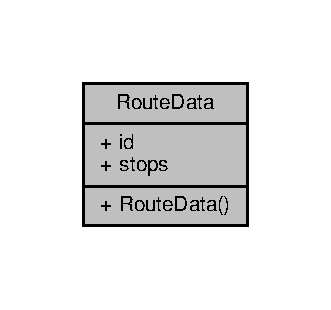
\includegraphics[width=159pt]{structRouteData__coll__graph}
\end{center}
\end{figure}
\subsection*{Public Attributes}
\begin{DoxyCompactItemize}
\item 
\mbox{\Hypertarget{structRouteData_a578af871a15d4737ab8d2074887da85f}\label{structRouteData_a578af871a15d4737ab8d2074887da85f}} 
std\+::string {\bfseries id}
\item 
\mbox{\Hypertarget{structRouteData_af867789789fbcfe97bdd554e56b121bf}\label{structRouteData_af867789789fbcfe97bdd554e56b121bf}} 
std\+::vector$<$ \hyperlink{structStopData}{Stop\+Data} $>$ {\bfseries stops}
\end{DoxyCompactItemize}


The documentation for this struct was generated from the following file\+:\begin{DoxyCompactItemize}
\item 
/home/wang8635/3081\+\_\+s20/repo-\/wang8635/project/src/data\+\_\+structs.\+h\end{DoxyCompactItemize}

\hypertarget{classSmallBus}{}\section{Small\+Bus Class Reference}
\label{classSmallBus}\index{Small\+Bus@{Small\+Bus}}


The main class for the generation of regular bus.  




{\ttfamily \#include $<$small\+\_\+bus.\+h$>$}



Inheritance diagram for Small\+Bus\+:\nopagebreak
\begin{figure}[H]
\begin{center}
\leavevmode
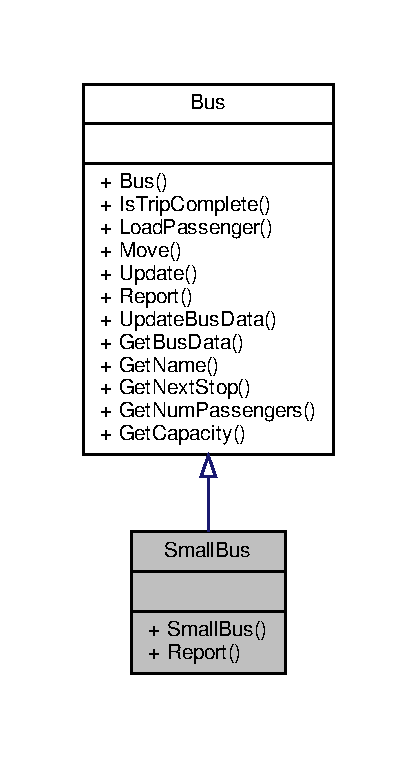
\includegraphics[width=200pt]{classSmallBus__inherit__graph}
\end{center}
\end{figure}


Collaboration diagram for Small\+Bus\+:\nopagebreak
\begin{figure}[H]
\begin{center}
\leavevmode
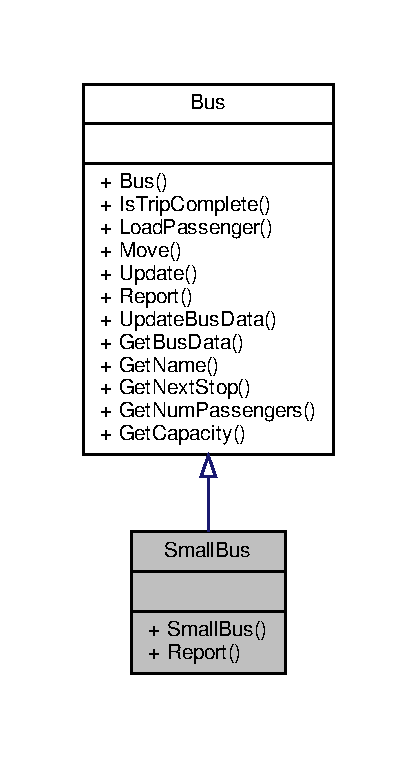
\includegraphics[width=200pt]{classSmallBus__coll__graph}
\end{center}
\end{figure}
\subsection*{Public Member Functions}
\begin{DoxyCompactItemize}
\item 
\hyperlink{classSmallBus_ab92bbfb8a88c33ffeabc685a6857820c}{Small\+Bus} (std\+::string name, \hyperlink{classRoute}{Route} $\ast$out, \hyperlink{classRoute}{Route} $\ast$in, int capacity, double speed)
\begin{DoxyCompactList}\small\item\em this class represent of generateor which randomly generate small bus. \end{DoxyCompactList}\item 
void \hyperlink{classSmallBus_a989198babc9a180799de58b4f3dadb50}{Report} (std\+::ostream \&)
\begin{DoxyCompactList}\small\item\em this class represent of generate 3 number that relate to 3 different buses. \end{DoxyCompactList}\end{DoxyCompactItemize}


\subsection{Detailed Description}
The main class for the generation of regular bus. 

Calls to Generate function to get a new instance of a bus. This is a static call, not requiring an instance to invoke the method. 

\subsection{Constructor \& Destructor Documentation}
\mbox{\Hypertarget{classSmallBus_ab92bbfb8a88c33ffeabc685a6857820c}\label{classSmallBus_ab92bbfb8a88c33ffeabc685a6857820c}} 
\index{Small\+Bus@{Small\+Bus}!Small\+Bus@{Small\+Bus}}
\index{Small\+Bus@{Small\+Bus}!Small\+Bus@{Small\+Bus}}
\subsubsection{\texorpdfstring{Small\+Bus()}{SmallBus()}}
{\footnotesize\ttfamily Small\+Bus\+::\+Small\+Bus (\begin{DoxyParamCaption}\item[{std\+::string}]{name,  }\item[{\hyperlink{classRoute}{Route} $\ast$}]{out,  }\item[{\hyperlink{classRoute}{Route} $\ast$}]{in,  }\item[{int}]{capacity,  }\item[{double}]{speed }\end{DoxyParamCaption})}



this class represent of generateor which randomly generate small bus. 

This function will be used for simulation purposes.


\begin{DoxyParams}[1]{Parameters}
\mbox{\tt in}  & {\em name} & bus id, left bound (not-\/inclusive) \\
\hline
\mbox{\tt in}  & {\em out} & outgoing route, right bound (inclusive) \\
\hline
\mbox{\tt in}  & {\em in} & incoming route, left bound (not-\/inclusive) \\
\hline
\mbox{\tt in}  & {\em capacity} & capacity of bus, right bound (inclusive) \\
\hline
\mbox{\tt in}  & {\em speed} & Speed of bus, left bound (not-\/inclusive)\\
\hline
\end{DoxyParams}
\begin{DoxyReturn}{Returns}
\hyperlink{classBus}{Bus} object with bus id, outgoing route, incoming route, small capacity, speed. 
\end{DoxyReturn}


\subsection{Member Function Documentation}
\mbox{\Hypertarget{classSmallBus_a989198babc9a180799de58b4f3dadb50}\label{classSmallBus_a989198babc9a180799de58b4f3dadb50}} 
\index{Small\+Bus@{Small\+Bus}!Report@{Report}}
\index{Report@{Report}!Small\+Bus@{Small\+Bus}}
\subsubsection{\texorpdfstring{Report()}{Report()}}
{\footnotesize\ttfamily void Small\+Bus\+::\+Report (\begin{DoxyParamCaption}\item[{std\+::ostream \&}]{out }\end{DoxyParamCaption})}



this class represent of generate 3 number that relate to 3 different buses. 


\begin{DoxyParams}[1]{Parameters}
\mbox{\tt in}  & {\em std\+::ostream\&,left} & bound (not-\/inclusive)\\
\hline
\end{DoxyParams}
\begin{DoxyReturn}{Returns}
output bus detail. 
\end{DoxyReturn}


The documentation for this class was generated from the following files\+:\begin{DoxyCompactItemize}
\item 
/home/wang8635/3081\+\_\+s20/repo-\/wang8635/project/src/small\+\_\+bus.\+h\item 
/home/wang8635/3081\+\_\+s20/repo-\/wang8635/project/src/small\+\_\+bus.\+cc\end{DoxyCompactItemize}

\hypertarget{classStop}{}\section{Stop Class Reference}
\label{classStop}\index{Stop@{Stop}}


Collaboration diagram for Stop\+:
\nopagebreak
\begin{figure}[H]
\begin{center}
\leavevmode
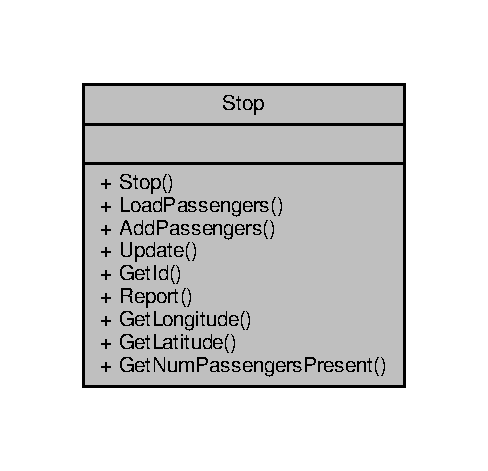
\includegraphics[width=234pt]{classStop__coll__graph}
\end{center}
\end{figure}
\subsection*{Public Member Functions}
\begin{DoxyCompactItemize}
\item 
\mbox{\Hypertarget{classStop_a59d881f072b1cf89512bb15a51ffc773}\label{classStop_a59d881f072b1cf89512bb15a51ffc773}} 
{\bfseries Stop} (int, double=44.\+973723, double=-\/93.\+235365)
\item 
\mbox{\Hypertarget{classStop_a02c6dcba2b6de5fdd008cf623f19bf7c}\label{classStop_a02c6dcba2b6de5fdd008cf623f19bf7c}} 
int {\bfseries Load\+Passengers} (\hyperlink{classBus}{Bus} $\ast$)
\item 
\mbox{\Hypertarget{classStop_a20a8b6035679d92a7a838a03a102bcd1}\label{classStop_a20a8b6035679d92a7a838a03a102bcd1}} 
int {\bfseries Add\+Passengers} (\hyperlink{classPassenger}{Passenger} $\ast$)
\item 
\mbox{\Hypertarget{classStop_aa373ae256ce6bc01ef13e876dfdec5bd}\label{classStop_aa373ae256ce6bc01ef13e876dfdec5bd}} 
void {\bfseries Update} ()
\item 
\mbox{\Hypertarget{classStop_a2f3b845d5a338f197226c90696314904}\label{classStop_a2f3b845d5a338f197226c90696314904}} 
int {\bfseries Get\+Id} () const
\item 
\mbox{\Hypertarget{classStop_a8e286b7cca2dce6977ebda6f01805d94}\label{classStop_a8e286b7cca2dce6977ebda6f01805d94}} 
void {\bfseries Report} (std\+::ostream \&) const
\item 
\mbox{\Hypertarget{classStop_a89e650eecf57c03ba0a5222bf5f666f5}\label{classStop_a89e650eecf57c03ba0a5222bf5f666f5}} 
double {\bfseries Get\+Longitude} () const
\item 
\mbox{\Hypertarget{classStop_a20ad94a1876baf31d8cf0708aae4d21f}\label{classStop_a20ad94a1876baf31d8cf0708aae4d21f}} 
double {\bfseries Get\+Latitude} () const
\item 
\mbox{\Hypertarget{classStop_a38b567326cfc072113b305a77a9e1315}\label{classStop_a38b567326cfc072113b305a77a9e1315}} 
size\+\_\+t {\bfseries Get\+Num\+Passengers\+Present} ()
\end{DoxyCompactItemize}


The documentation for this class was generated from the following files\+:\begin{DoxyCompactItemize}
\item 
/home/wang8635/3081\+\_\+s20/repo-\/wang8635/project/src/stop.\+h\item 
/home/wang8635/3081\+\_\+s20/repo-\/wang8635/project/src/\hyperlink{stop_8cc}{stop.\+cc}\end{DoxyCompactItemize}

\hypertarget{structStopData}{}\section{Stop\+Data Struct Reference}
\label{structStopData}\index{Stop\+Data@{Stop\+Data}}


Collaboration diagram for Stop\+Data\+:
\nopagebreak
\begin{figure}[H]
\begin{center}
\leavevmode
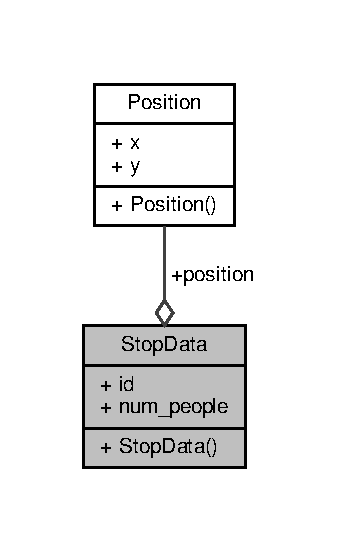
\includegraphics[width=162pt]{structStopData__coll__graph}
\end{center}
\end{figure}
\subsection*{Public Attributes}
\begin{DoxyCompactItemize}
\item 
\mbox{\Hypertarget{structStopData_abf63e623637d887c203c2a02b0855bb4}\label{structStopData_abf63e623637d887c203c2a02b0855bb4}} 
std\+::string {\bfseries id}
\item 
\mbox{\Hypertarget{structStopData_ae2e45d96bcd5b5f262796a6200a14fda}\label{structStopData_ae2e45d96bcd5b5f262796a6200a14fda}} 
\hyperlink{structPosition}{Position} {\bfseries position}
\item 
\mbox{\Hypertarget{structStopData_ac8346b0259972f304061a205d3f75f80}\label{structStopData_ac8346b0259972f304061a205d3f75f80}} 
int {\bfseries num\+\_\+people}
\end{DoxyCompactItemize}


The documentation for this struct was generated from the following file\+:\begin{DoxyCompactItemize}
\item 
/home/wang8635/3081\+\_\+s20/repo-\/wang8635/project/src/data\+\_\+structs.\+h\end{DoxyCompactItemize}

\chapter{File Documentation}
\hypertarget{bus_8cc}{}\section{/home/wang8635/3081\+\_\+s20/repo-\/wang8635/project/src/bus.cc File Reference}
\label{bus_8cc}\index{/home/wang8635/3081\+\_\+s20/repo-\/wang8635/project/src/bus.\+cc@{/home/wang8635/3081\+\_\+s20/repo-\/wang8635/project/src/bus.\+cc}}
{\ttfamily \#include \char`\"{}src/bus.\+h\char`\"{}}\newline
Include dependency graph for bus.\+cc\+:
\nopagebreak
\begin{figure}[H]
\begin{center}
\leavevmode
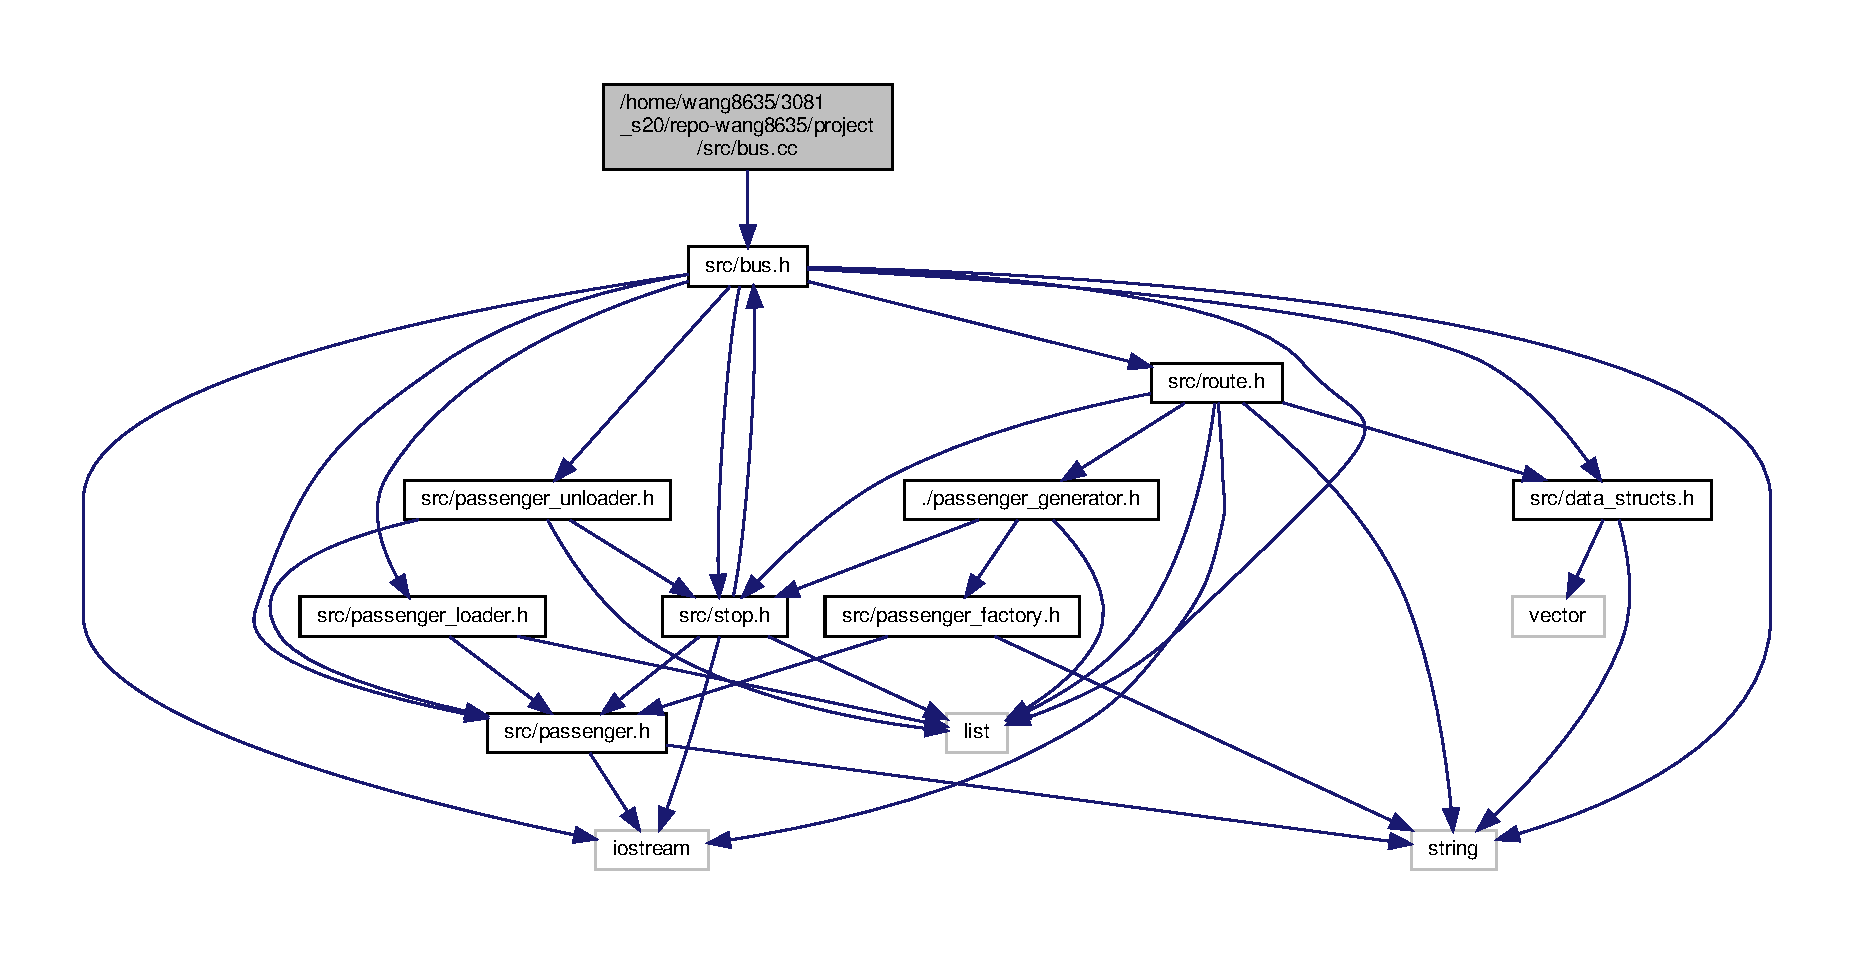
\includegraphics[width=350pt]{bus_8cc__incl}
\end{center}
\end{figure}


\subsection{Detailed Description}
\begin{DoxyCopyright}{Copyright}
2019 3081 Staff, All rights reserved. 
\end{DoxyCopyright}

\hypertarget{bus_8h}{}\section{/home/wang8635/3081\+\_\+s20/repo-\/wang8635/project/src/bus.h File Reference}
\label{bus_8h}\index{/home/wang8635/3081\+\_\+s20/repo-\/wang8635/project/src/bus.\+h@{/home/wang8635/3081\+\_\+s20/repo-\/wang8635/project/src/bus.\+h}}
{\ttfamily \#include $<$iostream$>$}\newline
{\ttfamily \#include $<$list$>$}\newline
{\ttfamily \#include $<$string$>$}\newline
{\ttfamily \#include \char`\"{}src/data\+\_\+structs.\+h\char`\"{}}\newline
{\ttfamily \#include \char`\"{}src/passenger.\+h\char`\"{}}\newline
{\ttfamily \#include \char`\"{}src/passenger\+\_\+loader.\+h\char`\"{}}\newline
{\ttfamily \#include \char`\"{}src/passenger\+\_\+unloader.\+h\char`\"{}}\newline
{\ttfamily \#include \char`\"{}src/route.\+h\char`\"{}}\newline
{\ttfamily \#include \char`\"{}src/stop.\+h\char`\"{}}\newline
Include dependency graph for bus.\+h\+:
\nopagebreak
\begin{figure}[H]
\begin{center}
\leavevmode
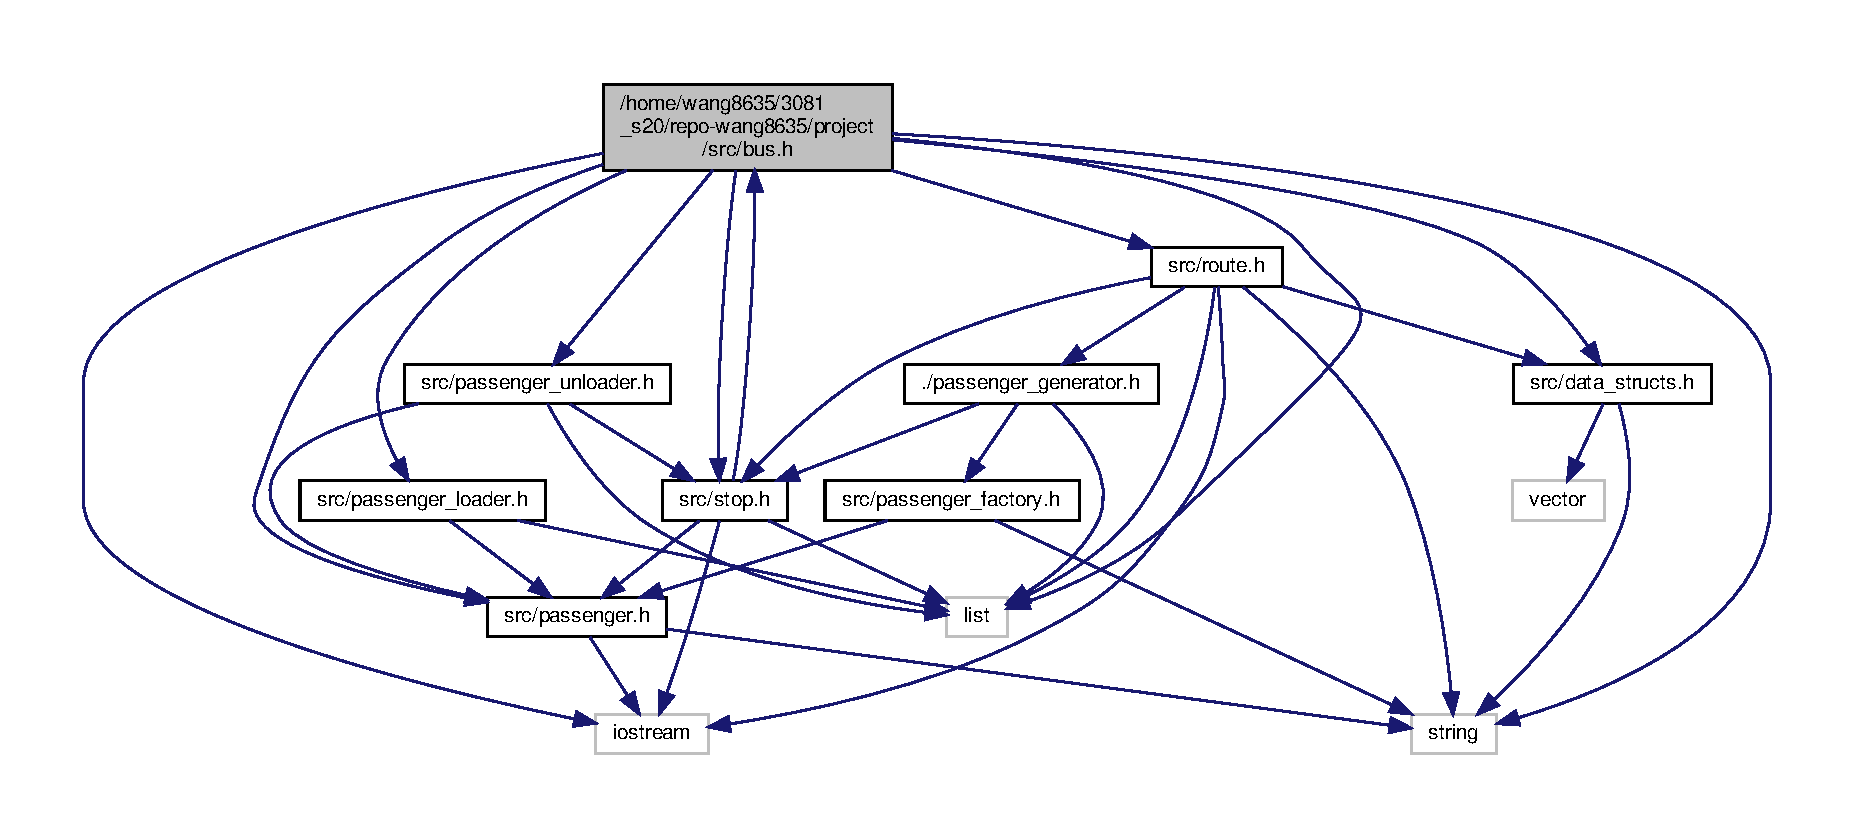
\includegraphics[width=350pt]{bus_8h__incl}
\end{center}
\end{figure}
This graph shows which files directly or indirectly include this file\+:
\nopagebreak
\begin{figure}[H]
\begin{center}
\leavevmode
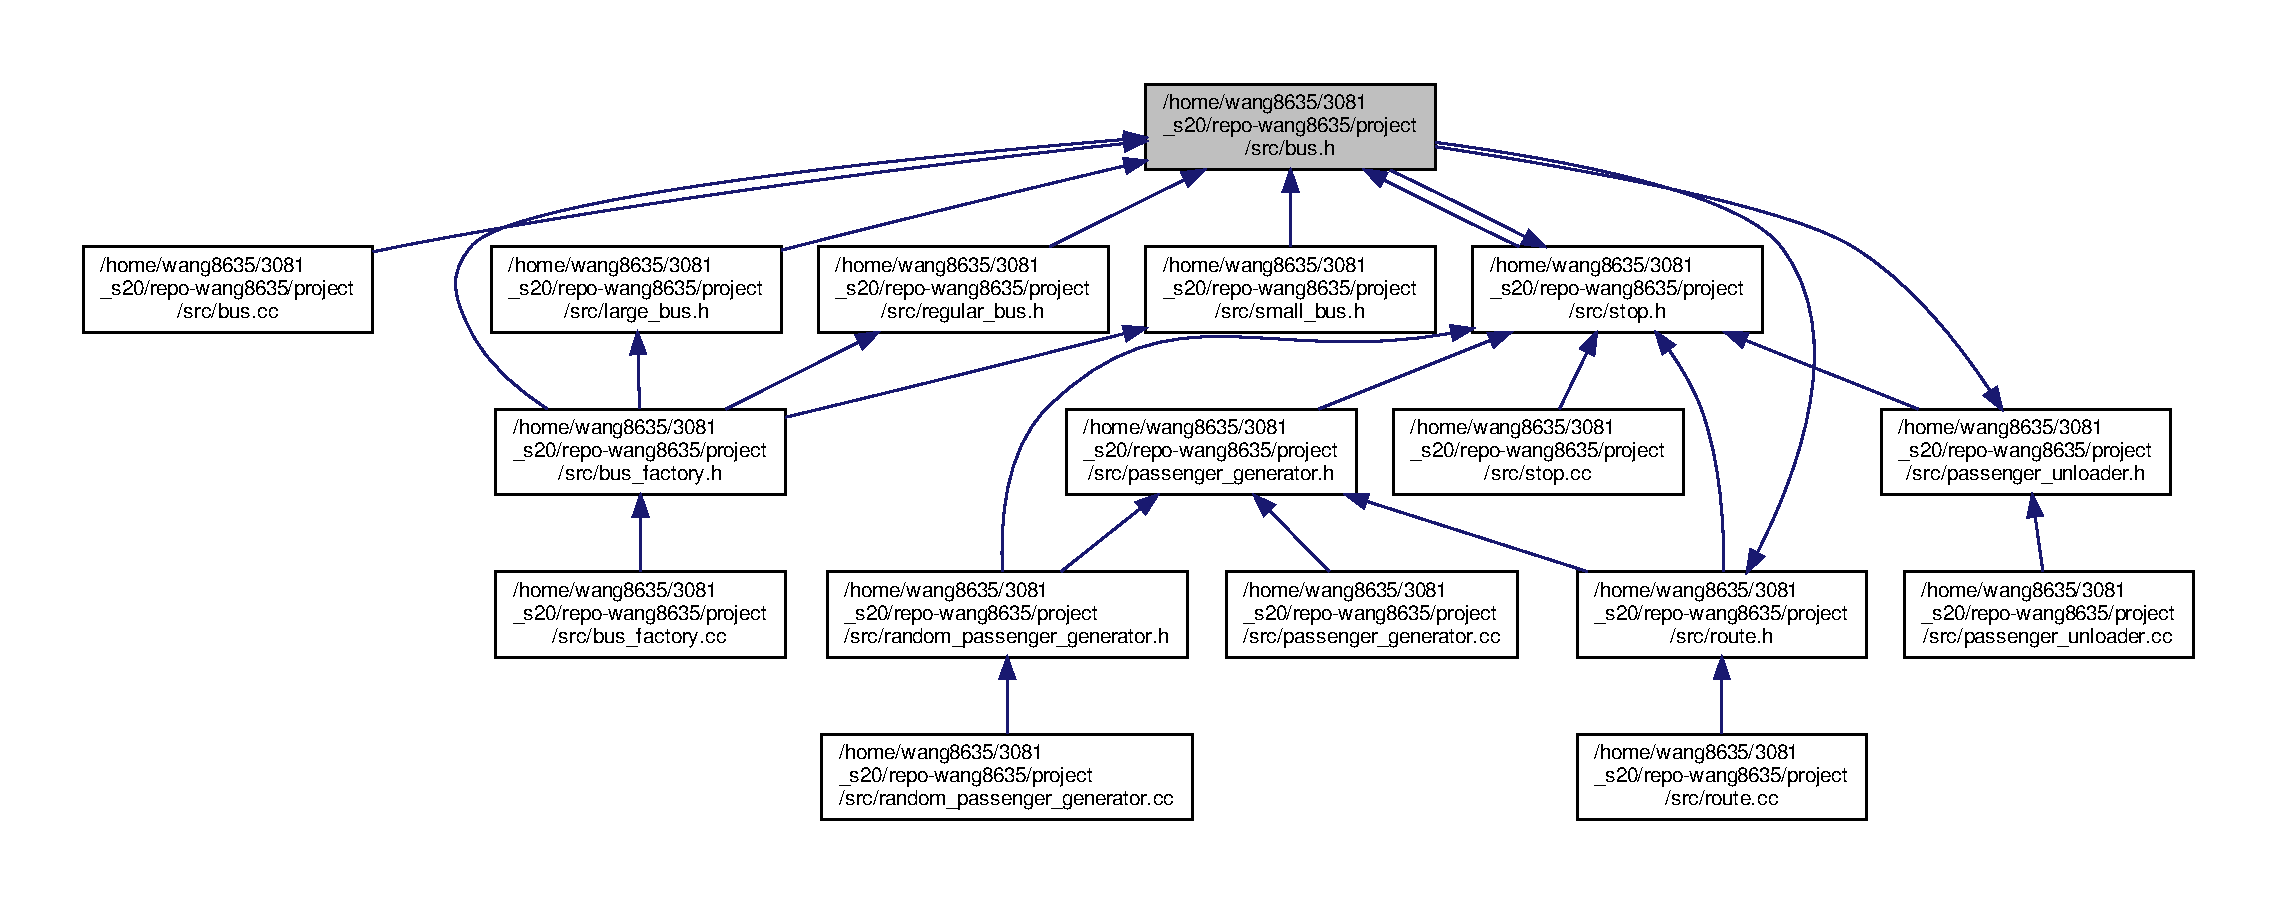
\includegraphics[width=350pt]{bus_8h__dep__incl}
\end{center}
\end{figure}
\subsection*{Classes}
\begin{DoxyCompactItemize}
\item 
class \hyperlink{classBus}{Bus}
\begin{DoxyCompactList}\small\item\em The main class for the bus. \end{DoxyCompactList}\end{DoxyCompactItemize}


\subsection{Detailed Description}
\begin{DoxyCopyright}{Copyright}
2019 3081 Staff, All rights reserved. 
\end{DoxyCopyright}

\hypertarget{bus__factory_8cc}{}\section{/home/wang8635/3081\+\_\+s20/repo-\/wang8635/project/src/bus\+\_\+factory.cc File Reference}
\label{bus__factory_8cc}\index{/home/wang8635/3081\+\_\+s20/repo-\/wang8635/project/src/bus\+\_\+factory.\+cc@{/home/wang8635/3081\+\_\+s20/repo-\/wang8635/project/src/bus\+\_\+factory.\+cc}}
{\ttfamily \#include $<$random$>$}\newline
{\ttfamily \#include $<$vector$>$}\newline
{\ttfamily \#include \char`\"{}src/bus\+\_\+factory.\+h\char`\"{}}\newline
Include dependency graph for bus\+\_\+factory.\+cc\+:\nopagebreak
\begin{figure}[H]
\begin{center}
\leavevmode
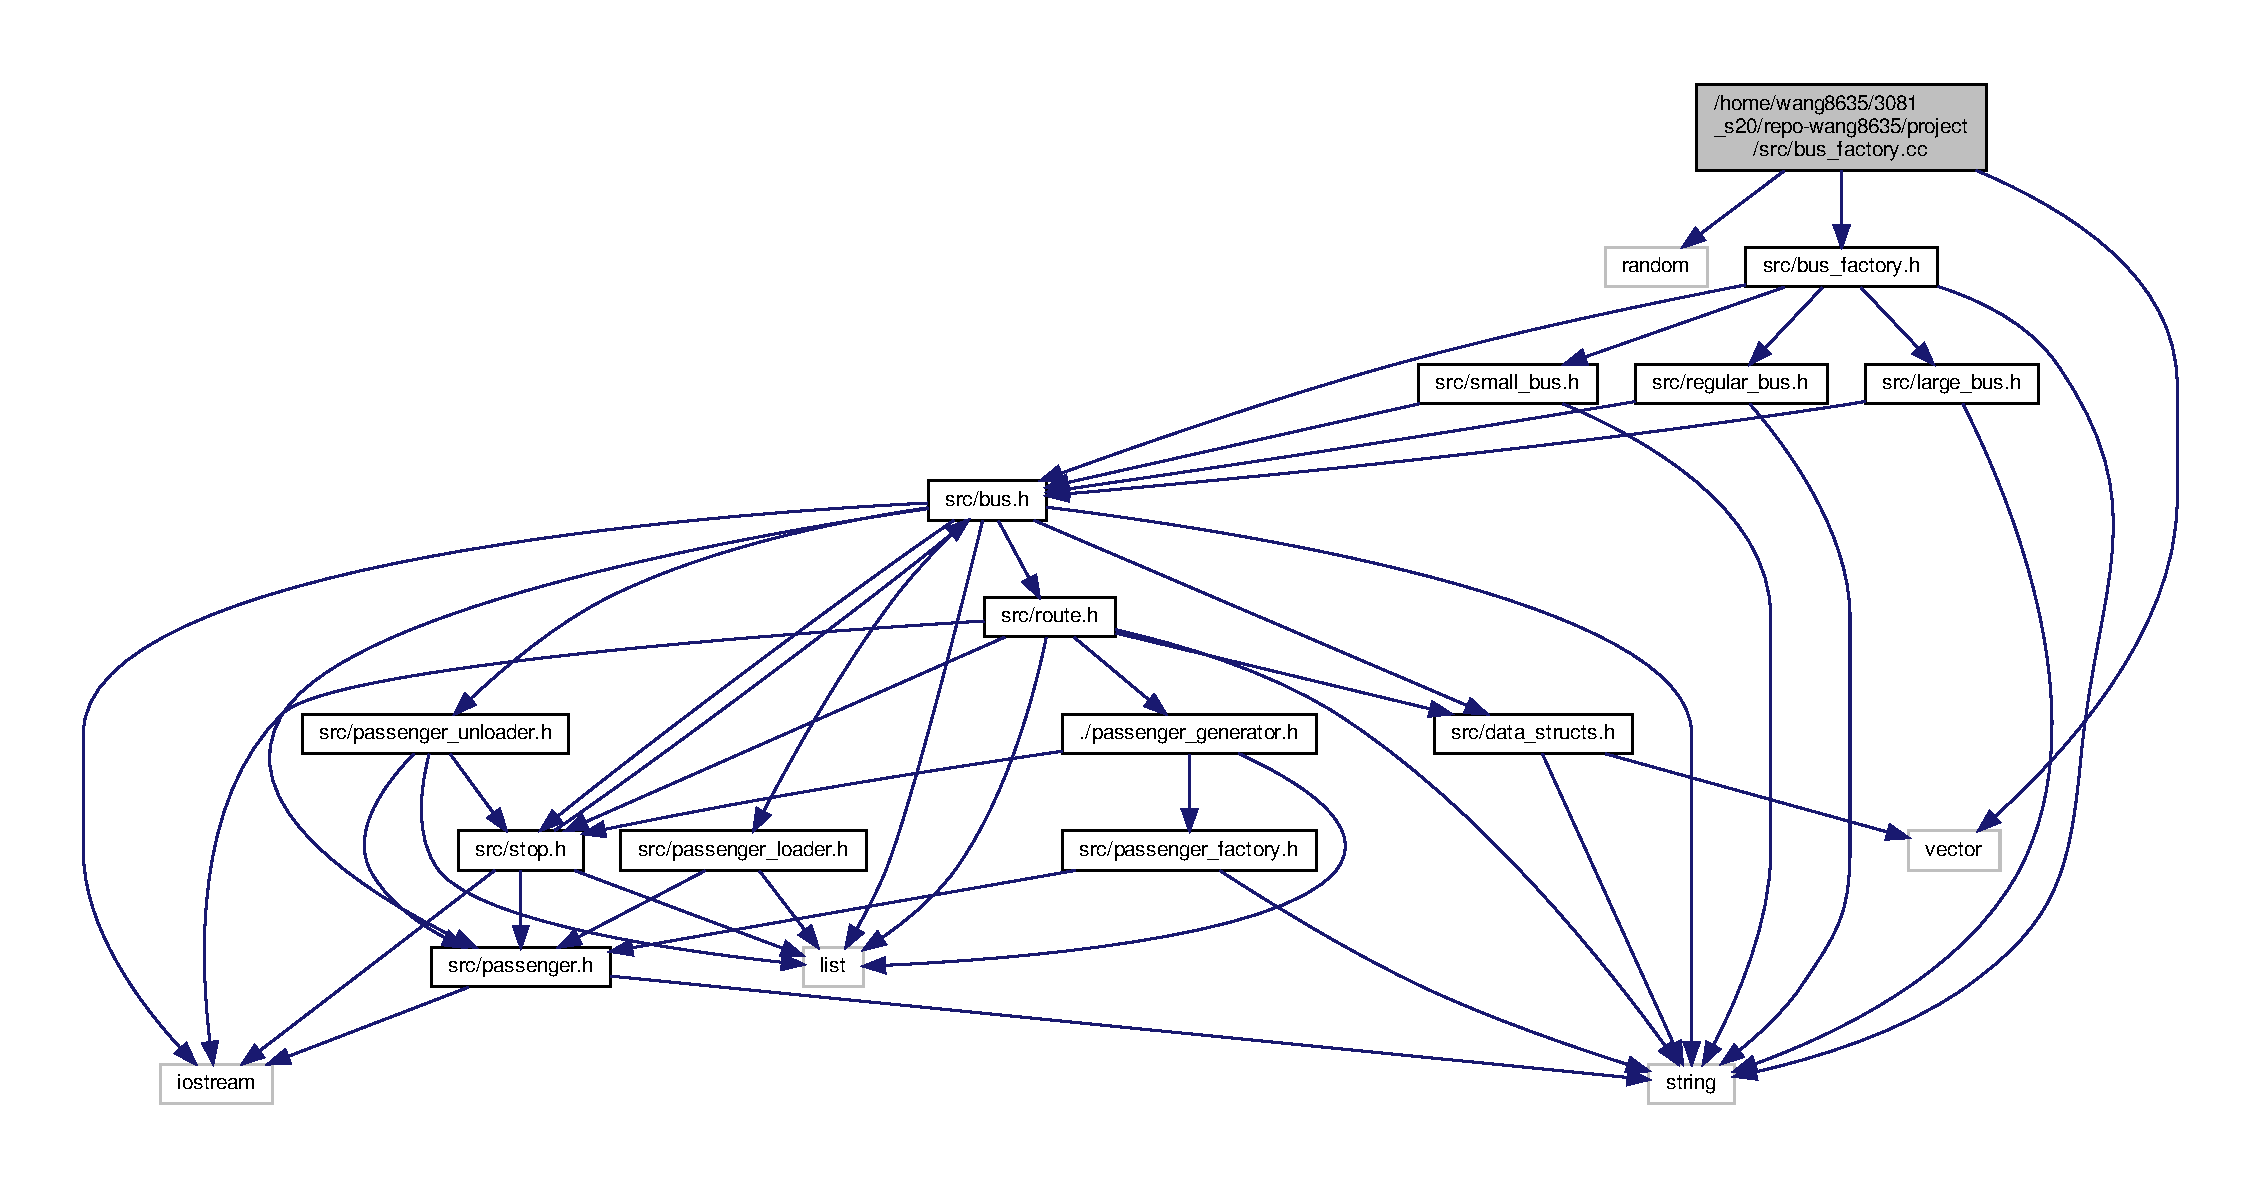
\includegraphics[width=350pt]{bus__factory_8cc__incl}
\end{center}
\end{figure}


\subsection{Detailed Description}
\begin{DoxyCopyright}{Copyright}
2019 3081 Staff, All rights reserved. 
\end{DoxyCopyright}

\hypertarget{bus__factory_8h}{}\section{/home/wang8635/3081\+\_\+s20/repo-\/wang8635/project/src/bus\+\_\+factory.h File Reference}
\label{bus__factory_8h}\index{/home/wang8635/3081\+\_\+s20/repo-\/wang8635/project/src/bus\+\_\+factory.\+h@{/home/wang8635/3081\+\_\+s20/repo-\/wang8635/project/src/bus\+\_\+factory.\+h}}
{\ttfamily \#include $<$string$>$}\newline
{\ttfamily \#include \char`\"{}src/bus.\+h\char`\"{}}\newline
{\ttfamily \#include \char`\"{}src/small\+\_\+bus.\+h\char`\"{}}\newline
{\ttfamily \#include \char`\"{}src/regular\+\_\+bus.\+h\char`\"{}}\newline
{\ttfamily \#include \char`\"{}src/large\+\_\+bus.\+h\char`\"{}}\newline
Include dependency graph for bus\+\_\+factory.\+h\+:
\nopagebreak
\begin{figure}[H]
\begin{center}
\leavevmode
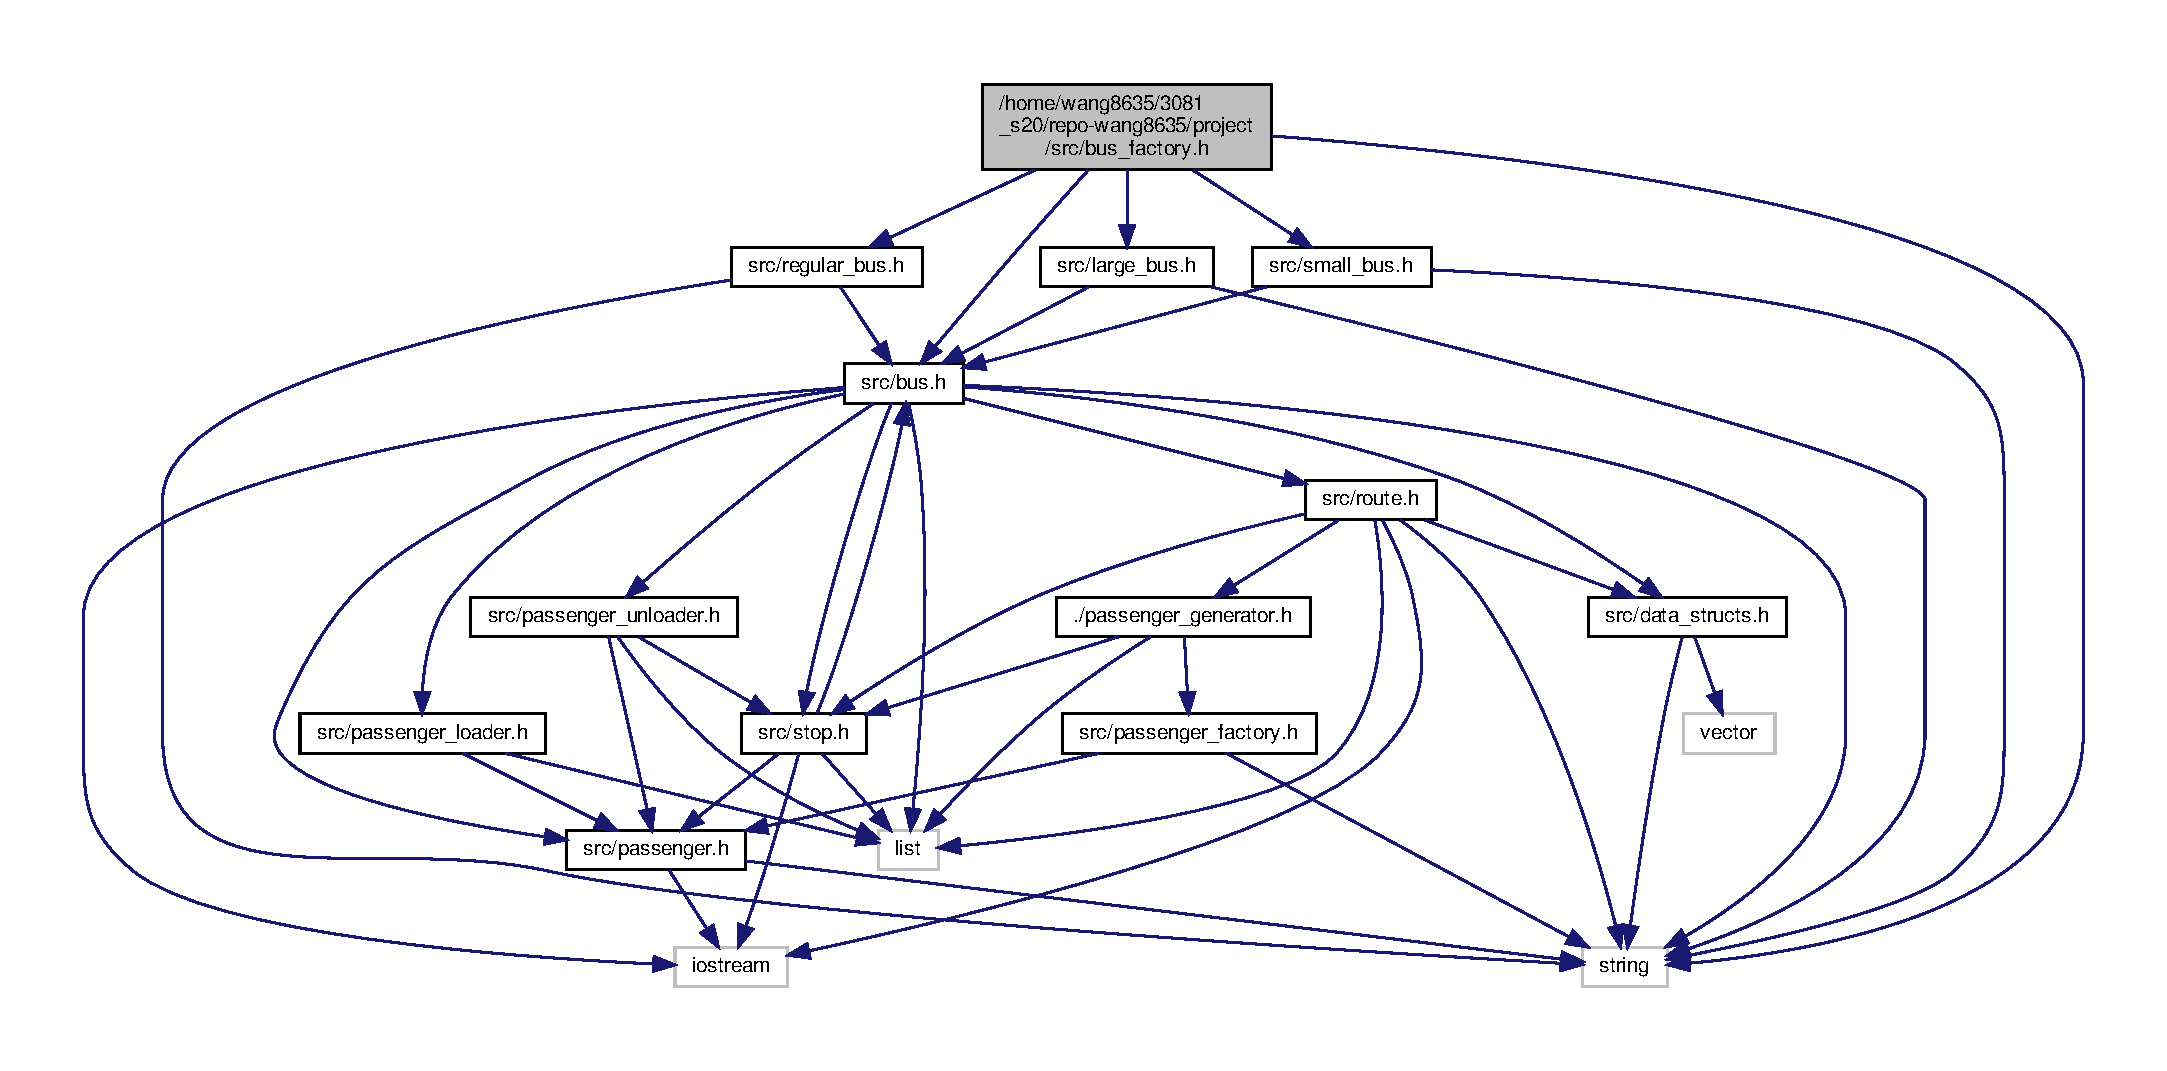
\includegraphics[width=350pt]{bus__factory_8h__incl}
\end{center}
\end{figure}
This graph shows which files directly or indirectly include this file\+:
\nopagebreak
\begin{figure}[H]
\begin{center}
\leavevmode
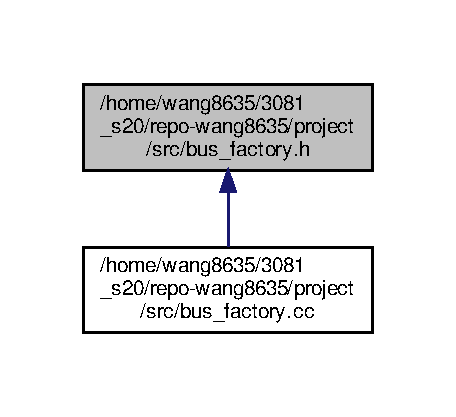
\includegraphics[width=219pt]{bus__factory_8h__dep__incl}
\end{center}
\end{figure}
\subsection*{Classes}
\begin{DoxyCompactItemize}
\item 
class \hyperlink{classBusFactory}{Bus\+Factory}
\begin{DoxyCompactList}\small\item\em The main class for the generation of bus. \end{DoxyCompactList}\end{DoxyCompactItemize}


\subsection{Detailed Description}
\begin{DoxyCopyright}{Copyright}
2019 3081 Staff, All rights reserved. 
\end{DoxyCopyright}

\hypertarget{passenger_8cc}{}\section{/home/wang8635/3081\+\_\+s20/repo-\/wang8635/project/src/passenger.cc File Reference}
\label{passenger_8cc}\index{/home/wang8635/3081\+\_\+s20/repo-\/wang8635/project/src/passenger.\+cc@{/home/wang8635/3081\+\_\+s20/repo-\/wang8635/project/src/passenger.\+cc}}
{\ttfamily \#include $<$iostream$>$}\newline
{\ttfamily \#include $<$string$>$}\newline
{\ttfamily \#include \char`\"{}src/passenger.\+h\char`\"{}}\newline
Include dependency graph for passenger.\+cc\+:
\nopagebreak
\begin{figure}[H]
\begin{center}
\leavevmode
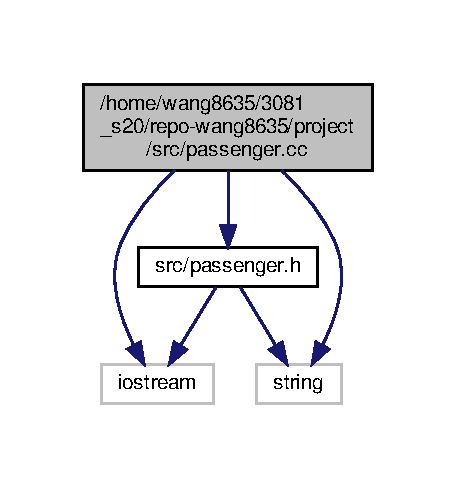
\includegraphics[width=219pt]{passenger_8cc__incl}
\end{center}
\end{figure}


\subsection{Detailed Description}
\begin{DoxyCopyright}{Copyright}
2019 3081 Staff, All rights reserved. 
\end{DoxyCopyright}

\hypertarget{passenger_8h}{}\section{/home/wang8635/3081\+\_\+s20/repo-\/wang8635/project/src/passenger.h File Reference}
\label{passenger_8h}\index{/home/wang8635/3081\+\_\+s20/repo-\/wang8635/project/src/passenger.\+h@{/home/wang8635/3081\+\_\+s20/repo-\/wang8635/project/src/passenger.\+h}}
{\ttfamily \#include $<$iostream$>$}\newline
{\ttfamily \#include $<$string$>$}\newline
Include dependency graph for passenger.\+h\+:\nopagebreak
\begin{figure}[H]
\begin{center}
\leavevmode
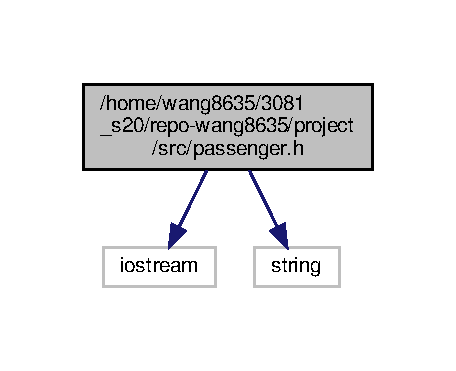
\includegraphics[width=219pt]{passenger_8h__incl}
\end{center}
\end{figure}
This graph shows which files directly or indirectly include this file\+:\nopagebreak
\begin{figure}[H]
\begin{center}
\leavevmode
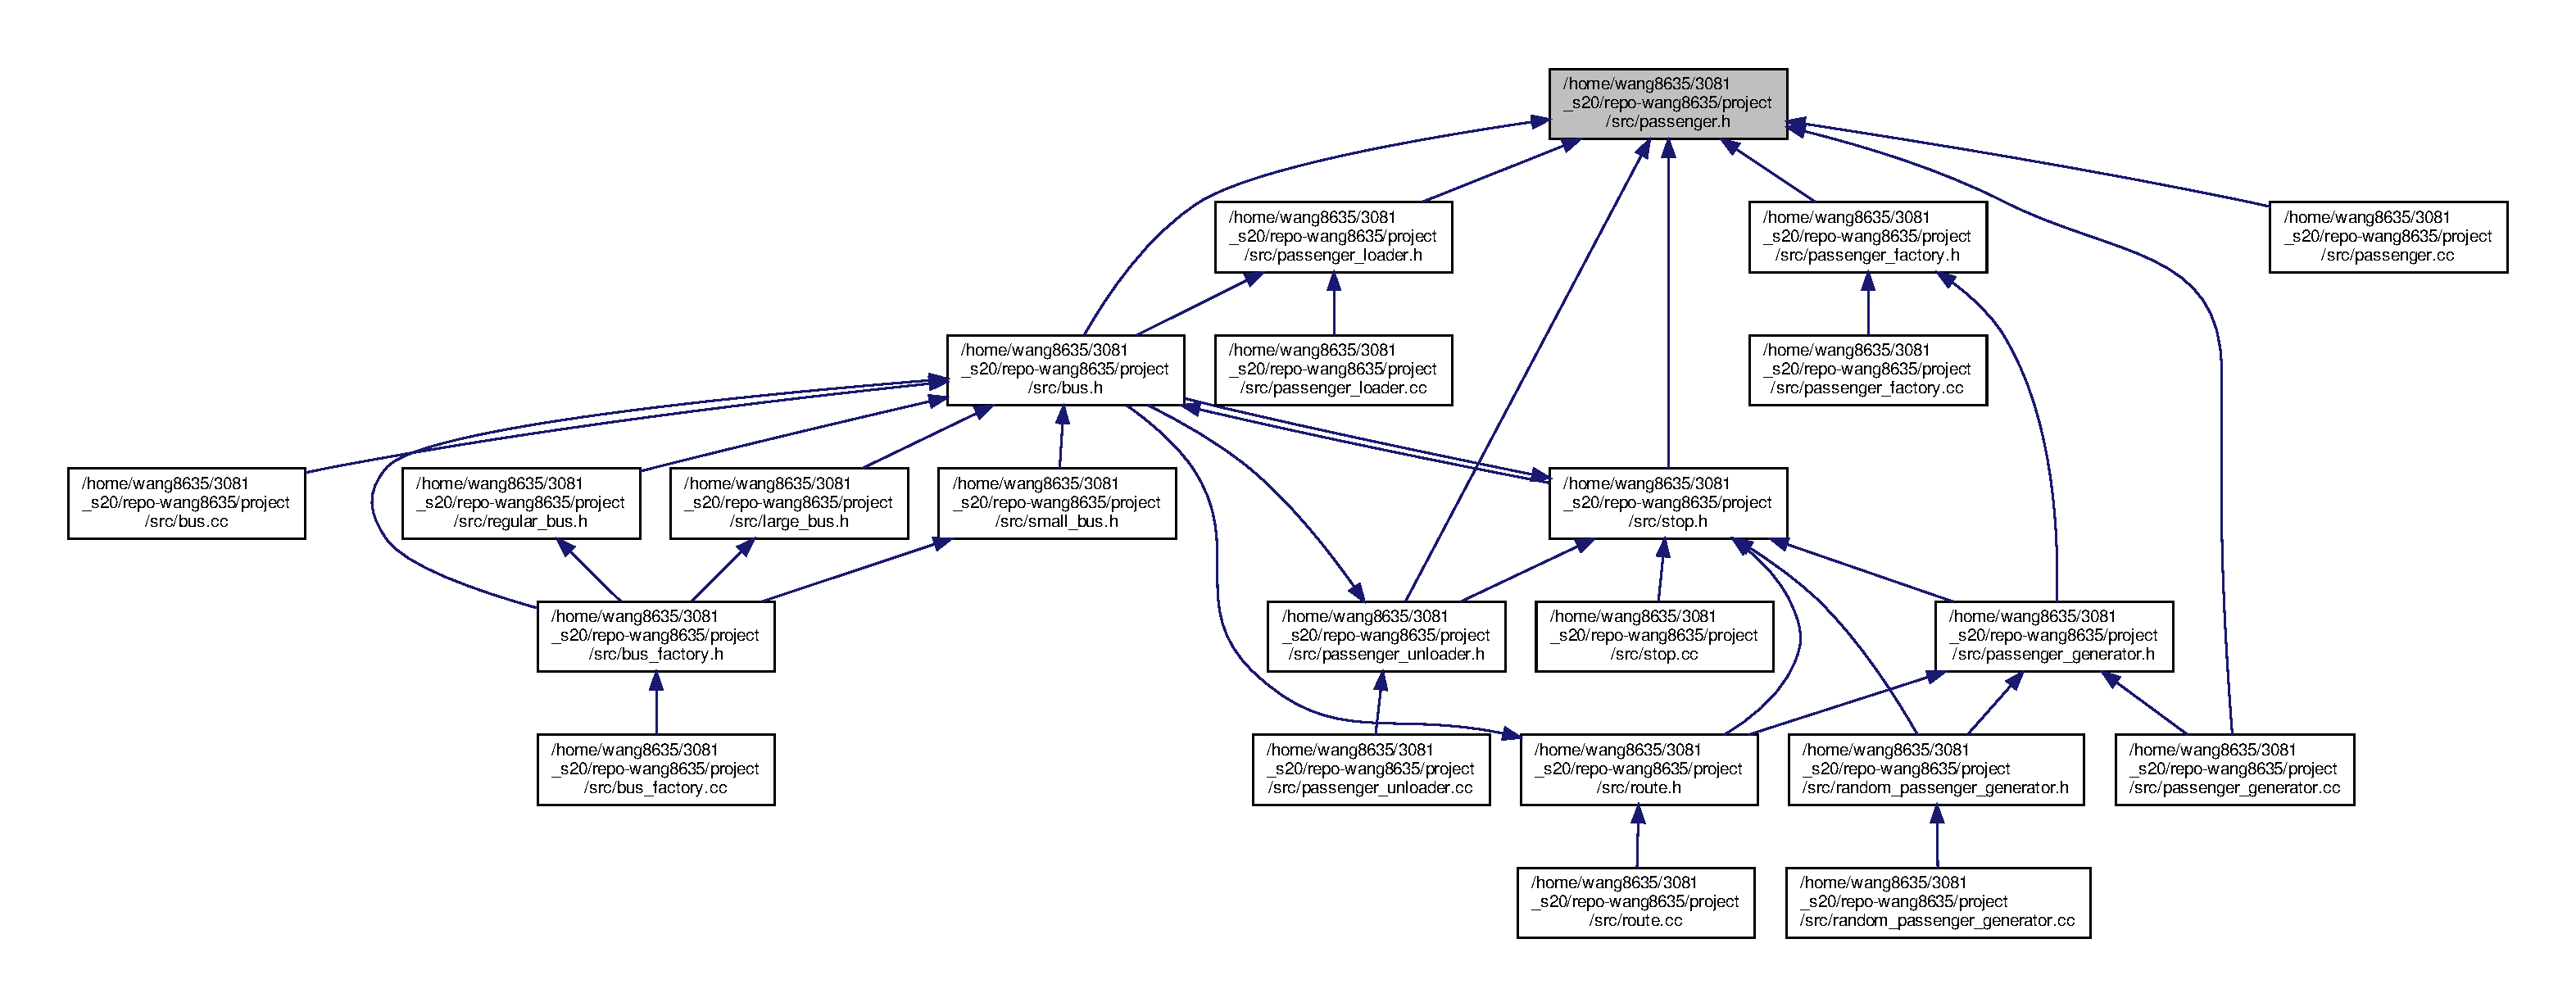
\includegraphics[width=350pt]{passenger_8h__dep__incl}
\end{center}
\end{figure}
\subsection*{Classes}
\begin{DoxyCompactItemize}
\item 
class \hyperlink{classPassenger}{Passenger}
\end{DoxyCompactItemize}


\subsection{Detailed Description}
\begin{DoxyCopyright}{Copyright}
2019 3081 Staff, All rights reserved. 
\end{DoxyCopyright}

\hypertarget{passenger__factory_8cc}{}\section{/home/wang8635/3081\+\_\+s20/repo-\/wang8635/project/src/passenger\+\_\+factory.cc File Reference}
\label{passenger__factory_8cc}\index{/home/wang8635/3081\+\_\+s20/repo-\/wang8635/project/src/passenger\+\_\+factory.\+cc@{/home/wang8635/3081\+\_\+s20/repo-\/wang8635/project/src/passenger\+\_\+factory.\+cc}}
{\ttfamily \#include $<$random$>$}\newline
{\ttfamily \#include $<$string$>$}\newline
{\ttfamily \#include \char`\"{}src/passenger\+\_\+factory.\+h\char`\"{}}\newline
Include dependency graph for passenger\+\_\+factory.\+cc\+:\nopagebreak
\begin{figure}[H]
\begin{center}
\leavevmode
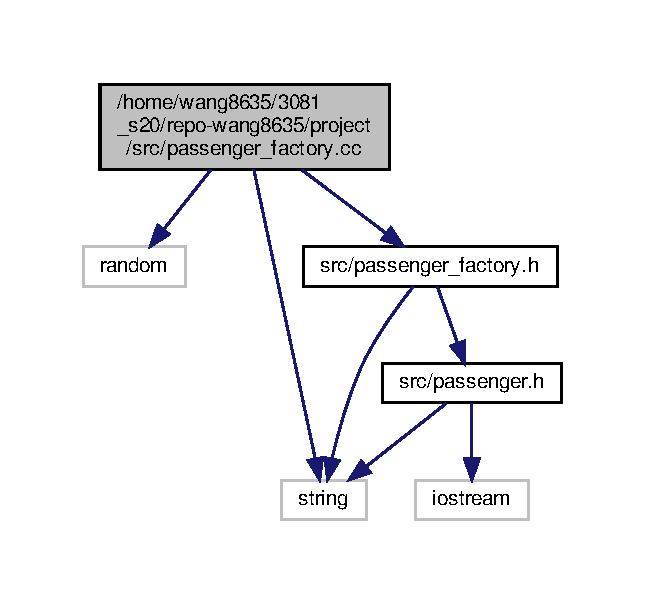
\includegraphics[width=310pt]{passenger__factory_8cc__incl}
\end{center}
\end{figure}
\subsection*{Functions}
\begin{DoxyCompactItemize}
\item 
\mbox{\Hypertarget{passenger__factory_8cc_af34adcff7354e7e8d172f7a97bc05d68}\label{passenger__factory_8cc_af34adcff7354e7e8d172f7a97bc05d68}} 
std\+::mt19937 {\bfseries e} (dev())
\item 
\mbox{\Hypertarget{passenger__factory_8cc_a1d818b31bbf5715a76ee321d8a0993e0}\label{passenger__factory_8cc_a1d818b31bbf5715a76ee321d8a0993e0}} 
std\+::uniform\+\_\+int\+\_\+distribution$<$ std\+::mt19937\+::result\+\_\+type $>$ {\bfseries dist} (1, 1000)
\end{DoxyCompactItemize}
\subsection*{Variables}
\begin{DoxyCompactItemize}
\item 
\mbox{\Hypertarget{passenger__factory_8cc_ad768868c172722a84c70801c1382438f}\label{passenger__factory_8cc_ad768868c172722a84c70801c1382438f}} 
std\+::random\+\_\+device {\bfseries dev}
\end{DoxyCompactItemize}


\subsection{Detailed Description}
\begin{DoxyCopyright}{Copyright}
2019 3081 Staff, All rights reserved. 
\end{DoxyCopyright}

\hypertarget{passenger__factory_8h}{}\section{/home/wang8635/3081\+\_\+s20/repo-\/wang8635/project/src/passenger\+\_\+factory.h File Reference}
\label{passenger__factory_8h}\index{/home/wang8635/3081\+\_\+s20/repo-\/wang8635/project/src/passenger\+\_\+factory.\+h@{/home/wang8635/3081\+\_\+s20/repo-\/wang8635/project/src/passenger\+\_\+factory.\+h}}
{\ttfamily \#include $<$string$>$}\newline
{\ttfamily \#include \char`\"{}src/passenger.\+h\char`\"{}}\newline
Include dependency graph for passenger\+\_\+factory.\+h\+:\nopagebreak
\begin{figure}[H]
\begin{center}
\leavevmode
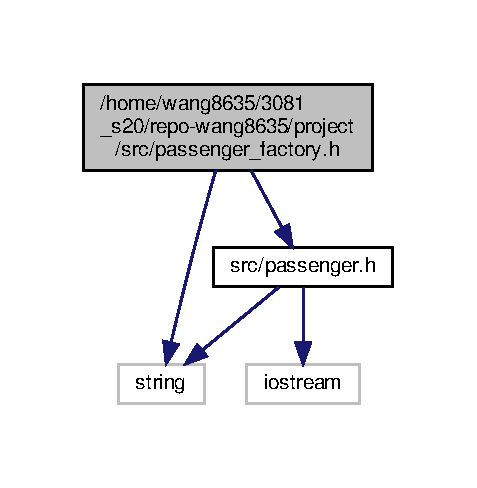
\includegraphics[width=229pt]{passenger__factory_8h__incl}
\end{center}
\end{figure}
This graph shows which files directly or indirectly include this file\+:\nopagebreak
\begin{figure}[H]
\begin{center}
\leavevmode
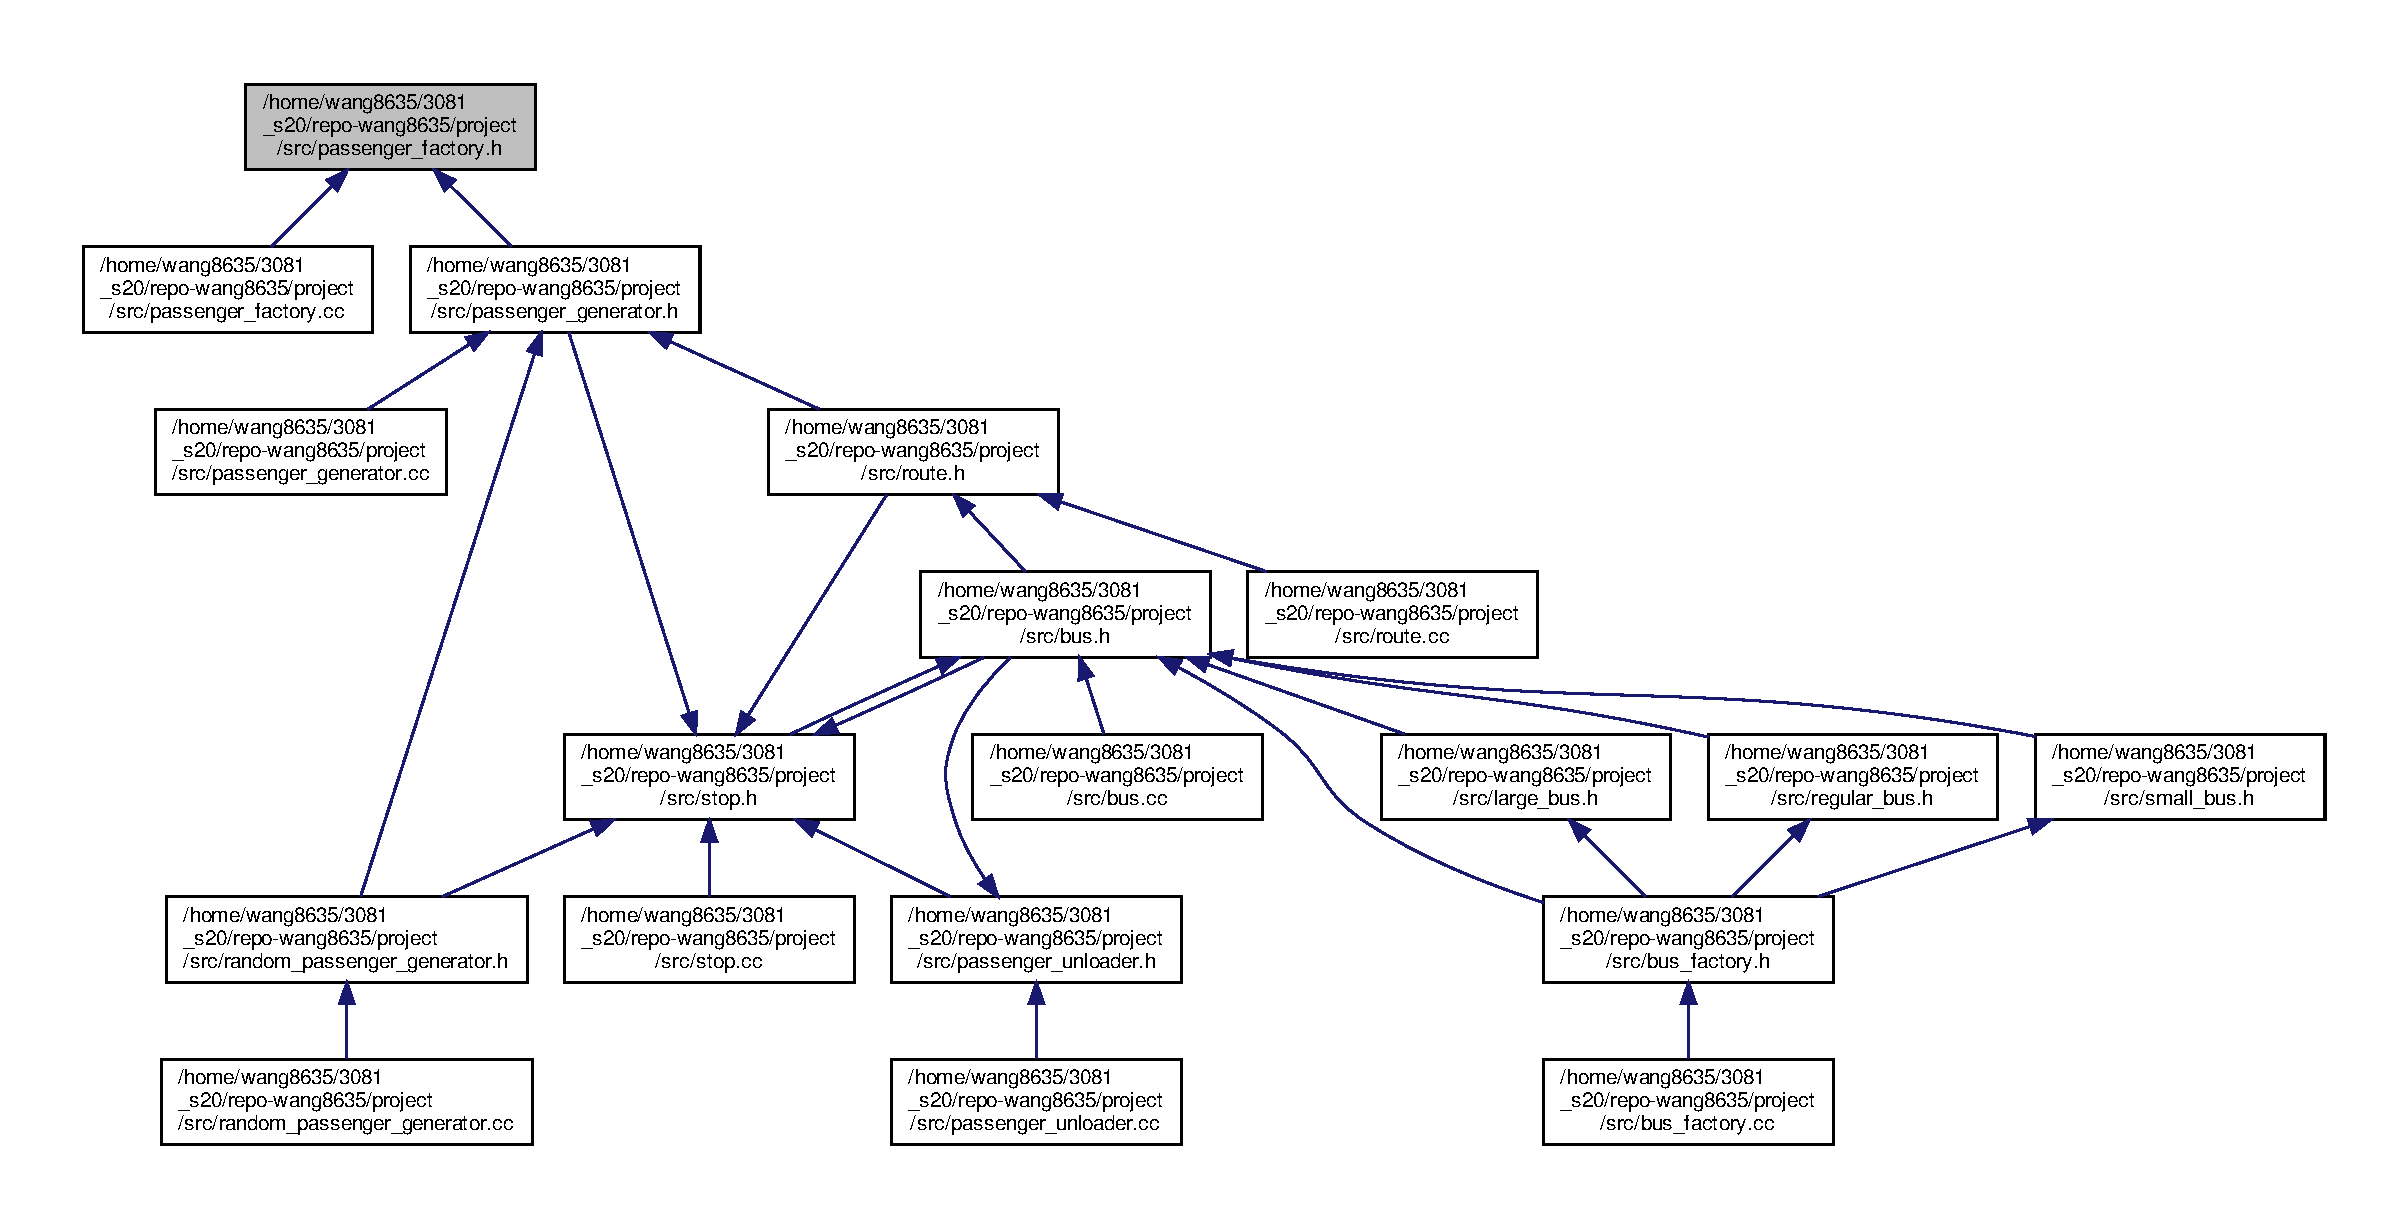
\includegraphics[width=350pt]{passenger__factory_8h__dep__incl}
\end{center}
\end{figure}
\subsection*{Classes}
\begin{DoxyCompactItemize}
\item 
class \hyperlink{classPassengerFactory}{Passenger\+Factory}
\end{DoxyCompactItemize}


\subsection{Detailed Description}
\begin{DoxyCopyright}{Copyright}
2019 3081 Staff, All rights reserved. 
\end{DoxyCopyright}

\hypertarget{passenger__generator_8cc}{}\section{/home/wang8635/3081\+\_\+s20/repo-\/wang8635/project/src/passenger\+\_\+generator.cc File Reference}
\label{passenger__generator_8cc}\index{/home/wang8635/3081\+\_\+s20/repo-\/wang8635/project/src/passenger\+\_\+generator.\+cc@{/home/wang8635/3081\+\_\+s20/repo-\/wang8635/project/src/passenger\+\_\+generator.\+cc}}
{\ttfamily \#include \char`\"{}src/passenger\+\_\+generator.\+h\char`\"{}}\newline
{\ttfamily \#include \char`\"{}src/passenger.\+h\char`\"{}}\newline
Include dependency graph for passenger\+\_\+generator.\+cc\+:\nopagebreak
\begin{figure}[H]
\begin{center}
\leavevmode
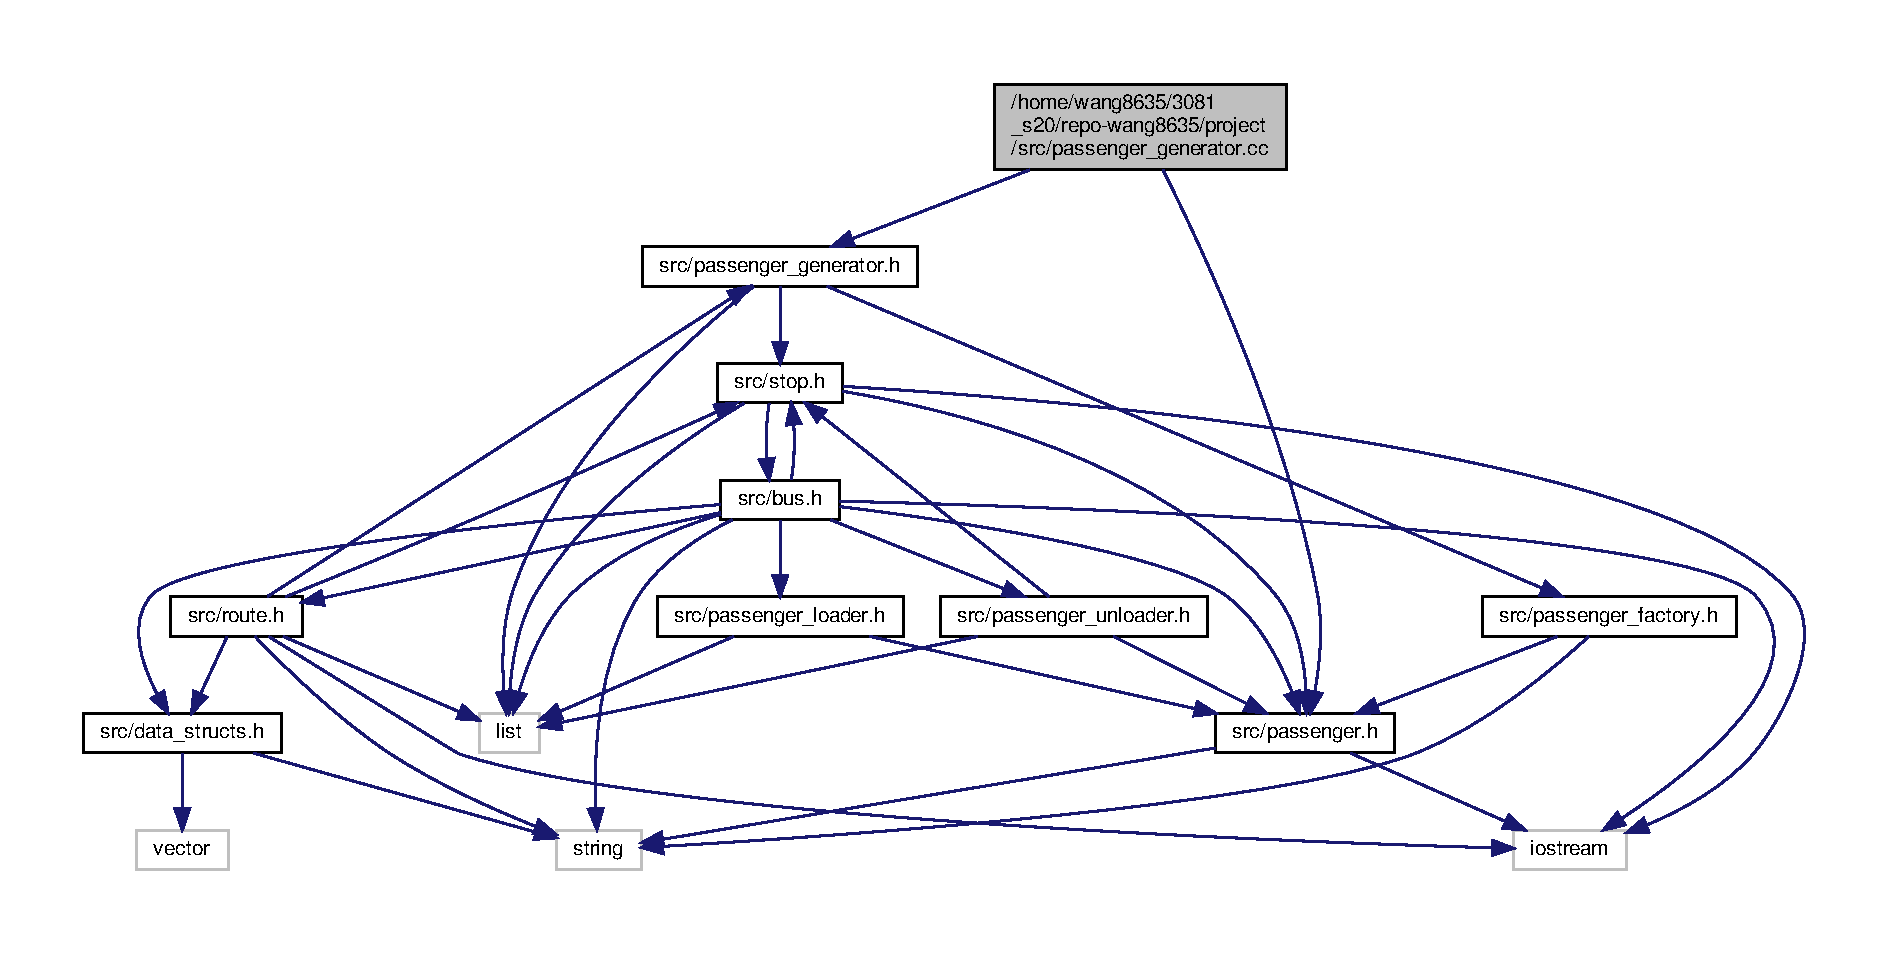
\includegraphics[width=350pt]{passenger__generator_8cc__incl}
\end{center}
\end{figure}


\subsection{Detailed Description}
\begin{DoxyCopyright}{Copyright}
2019 3081 Staff, All rights reserved. 
\end{DoxyCopyright}

\hypertarget{passenger__generator_8h}{}\section{/home/wang8635/3081\+\_\+s20/repo-\/wang8635/project/src/passenger\+\_\+generator.h File Reference}
\label{passenger__generator_8h}\index{/home/wang8635/3081\+\_\+s20/repo-\/wang8635/project/src/passenger\+\_\+generator.\+h@{/home/wang8635/3081\+\_\+s20/repo-\/wang8635/project/src/passenger\+\_\+generator.\+h}}
{\ttfamily \#include $<$list$>$}\newline
{\ttfamily \#include \char`\"{}src/passenger\+\_\+factory.\+h\char`\"{}}\newline
{\ttfamily \#include \char`\"{}src/stop.\+h\char`\"{}}\newline
Include dependency graph for passenger\+\_\+generator.\+h\+:
\nopagebreak
\begin{figure}[H]
\begin{center}
\leavevmode
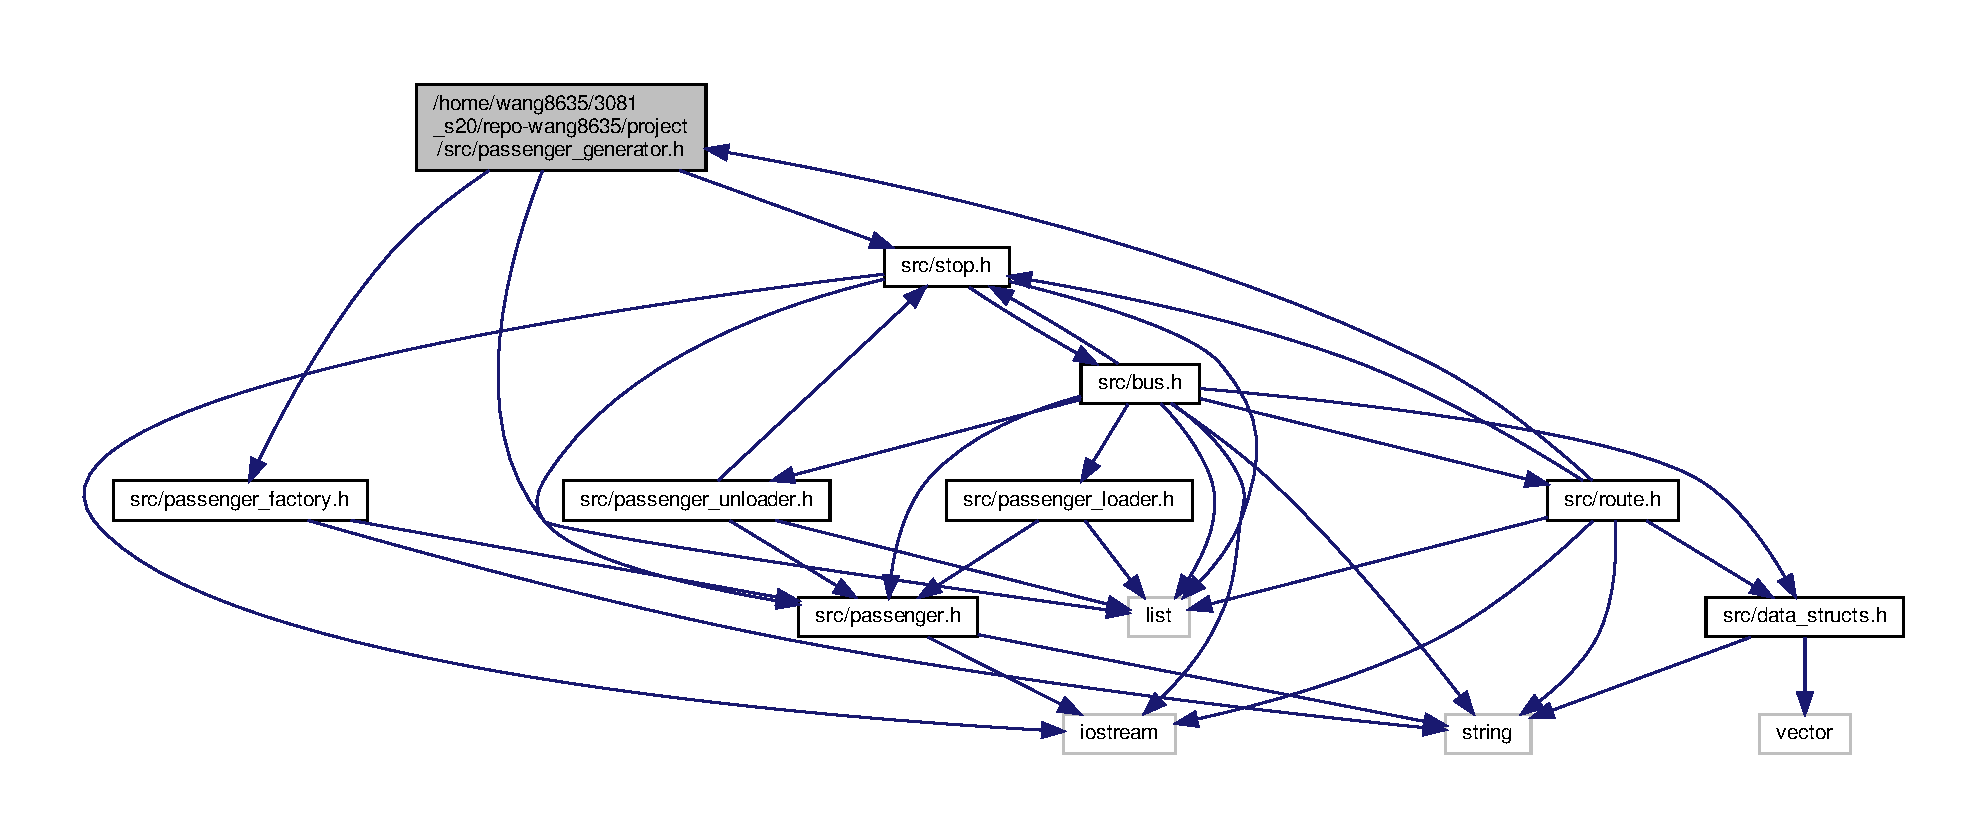
\includegraphics[width=350pt]{passenger__generator_8h__incl}
\end{center}
\end{figure}
This graph shows which files directly or indirectly include this file\+:
\nopagebreak
\begin{figure}[H]
\begin{center}
\leavevmode
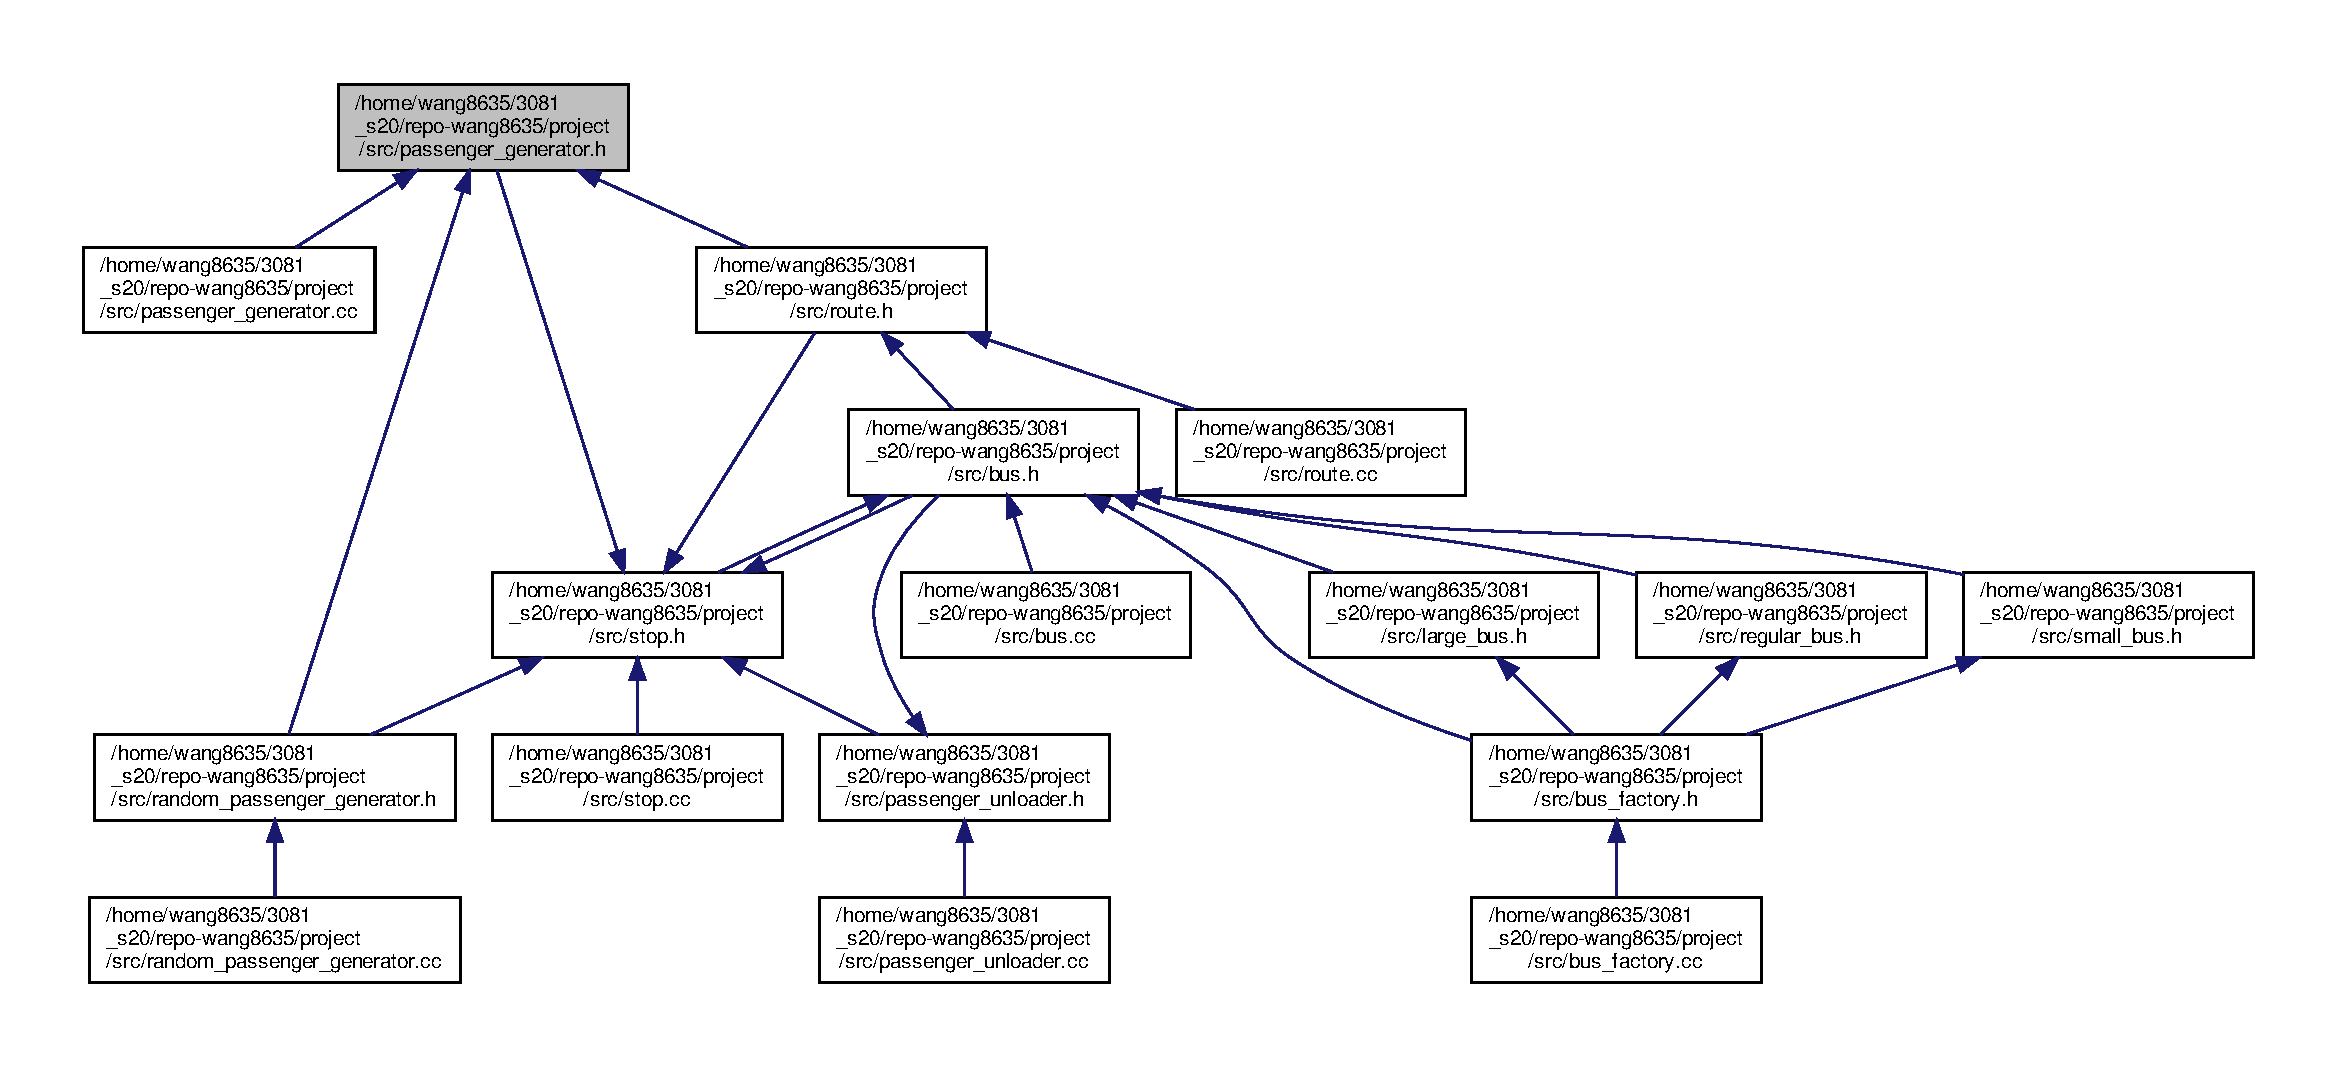
\includegraphics[width=350pt]{passenger__generator_8h__dep__incl}
\end{center}
\end{figure}
\subsection*{Classes}
\begin{DoxyCompactItemize}
\item 
class \hyperlink{classPassengerGenerator}{Passenger\+Generator}
\end{DoxyCompactItemize}


\subsection{Detailed Description}
\begin{DoxyCopyright}{Copyright}
2019 3081 Staff, All rights reserved. 
\end{DoxyCopyright}

\hypertarget{passenger__loader_8cc}{}\section{/home/wang8635/3081\+\_\+s20/repo-\/wang8635/project/src/passenger\+\_\+loader.cc File Reference}
\label{passenger__loader_8cc}\index{/home/wang8635/3081\+\_\+s20/repo-\/wang8635/project/src/passenger\+\_\+loader.\+cc@{/home/wang8635/3081\+\_\+s20/repo-\/wang8635/project/src/passenger\+\_\+loader.\+cc}}
{\ttfamily \#include \char`\"{}src/passenger\+\_\+loader.\+h\char`\"{}}\newline
Include dependency graph for passenger\+\_\+loader.\+cc\+:\nopagebreak
\begin{figure}[H]
\begin{center}
\leavevmode
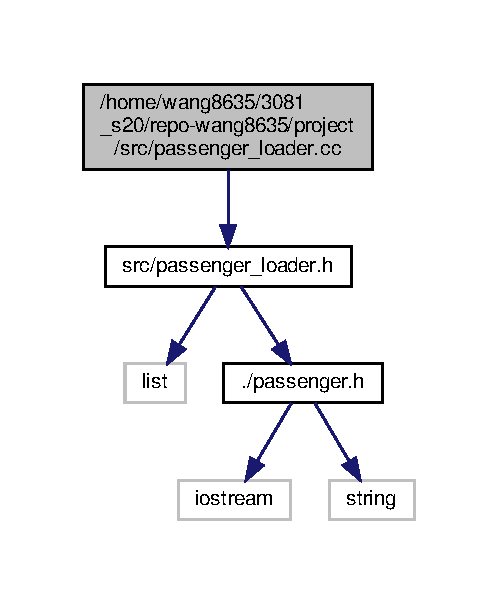
\includegraphics[width=239pt]{passenger__loader_8cc__incl}
\end{center}
\end{figure}


\subsection{Detailed Description}
\begin{DoxyCopyright}{Copyright}
2019 3081 Staff, All rights reserved. 
\end{DoxyCopyright}

\hypertarget{passenger__loader_8h}{}\section{/home/wang8635/3081\+\_\+s20/repo-\/wang8635/project/src/passenger\+\_\+loader.h File Reference}
\label{passenger__loader_8h}\index{/home/wang8635/3081\+\_\+s20/repo-\/wang8635/project/src/passenger\+\_\+loader.\+h@{/home/wang8635/3081\+\_\+s20/repo-\/wang8635/project/src/passenger\+\_\+loader.\+h}}
{\ttfamily \#include $<$list$>$}\newline
{\ttfamily \#include \char`\"{}./passenger.\+h\char`\"{}}\newline
Include dependency graph for passenger\+\_\+loader.\+h\+:\nopagebreak
\begin{figure}[H]
\begin{center}
\leavevmode
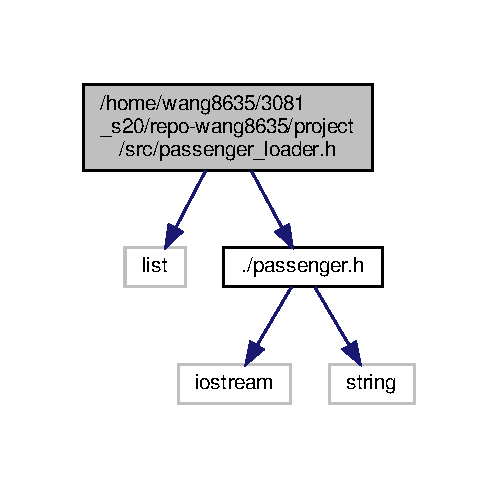
\includegraphics[width=239pt]{passenger__loader_8h__incl}
\end{center}
\end{figure}
This graph shows which files directly or indirectly include this file\+:\nopagebreak
\begin{figure}[H]
\begin{center}
\leavevmode
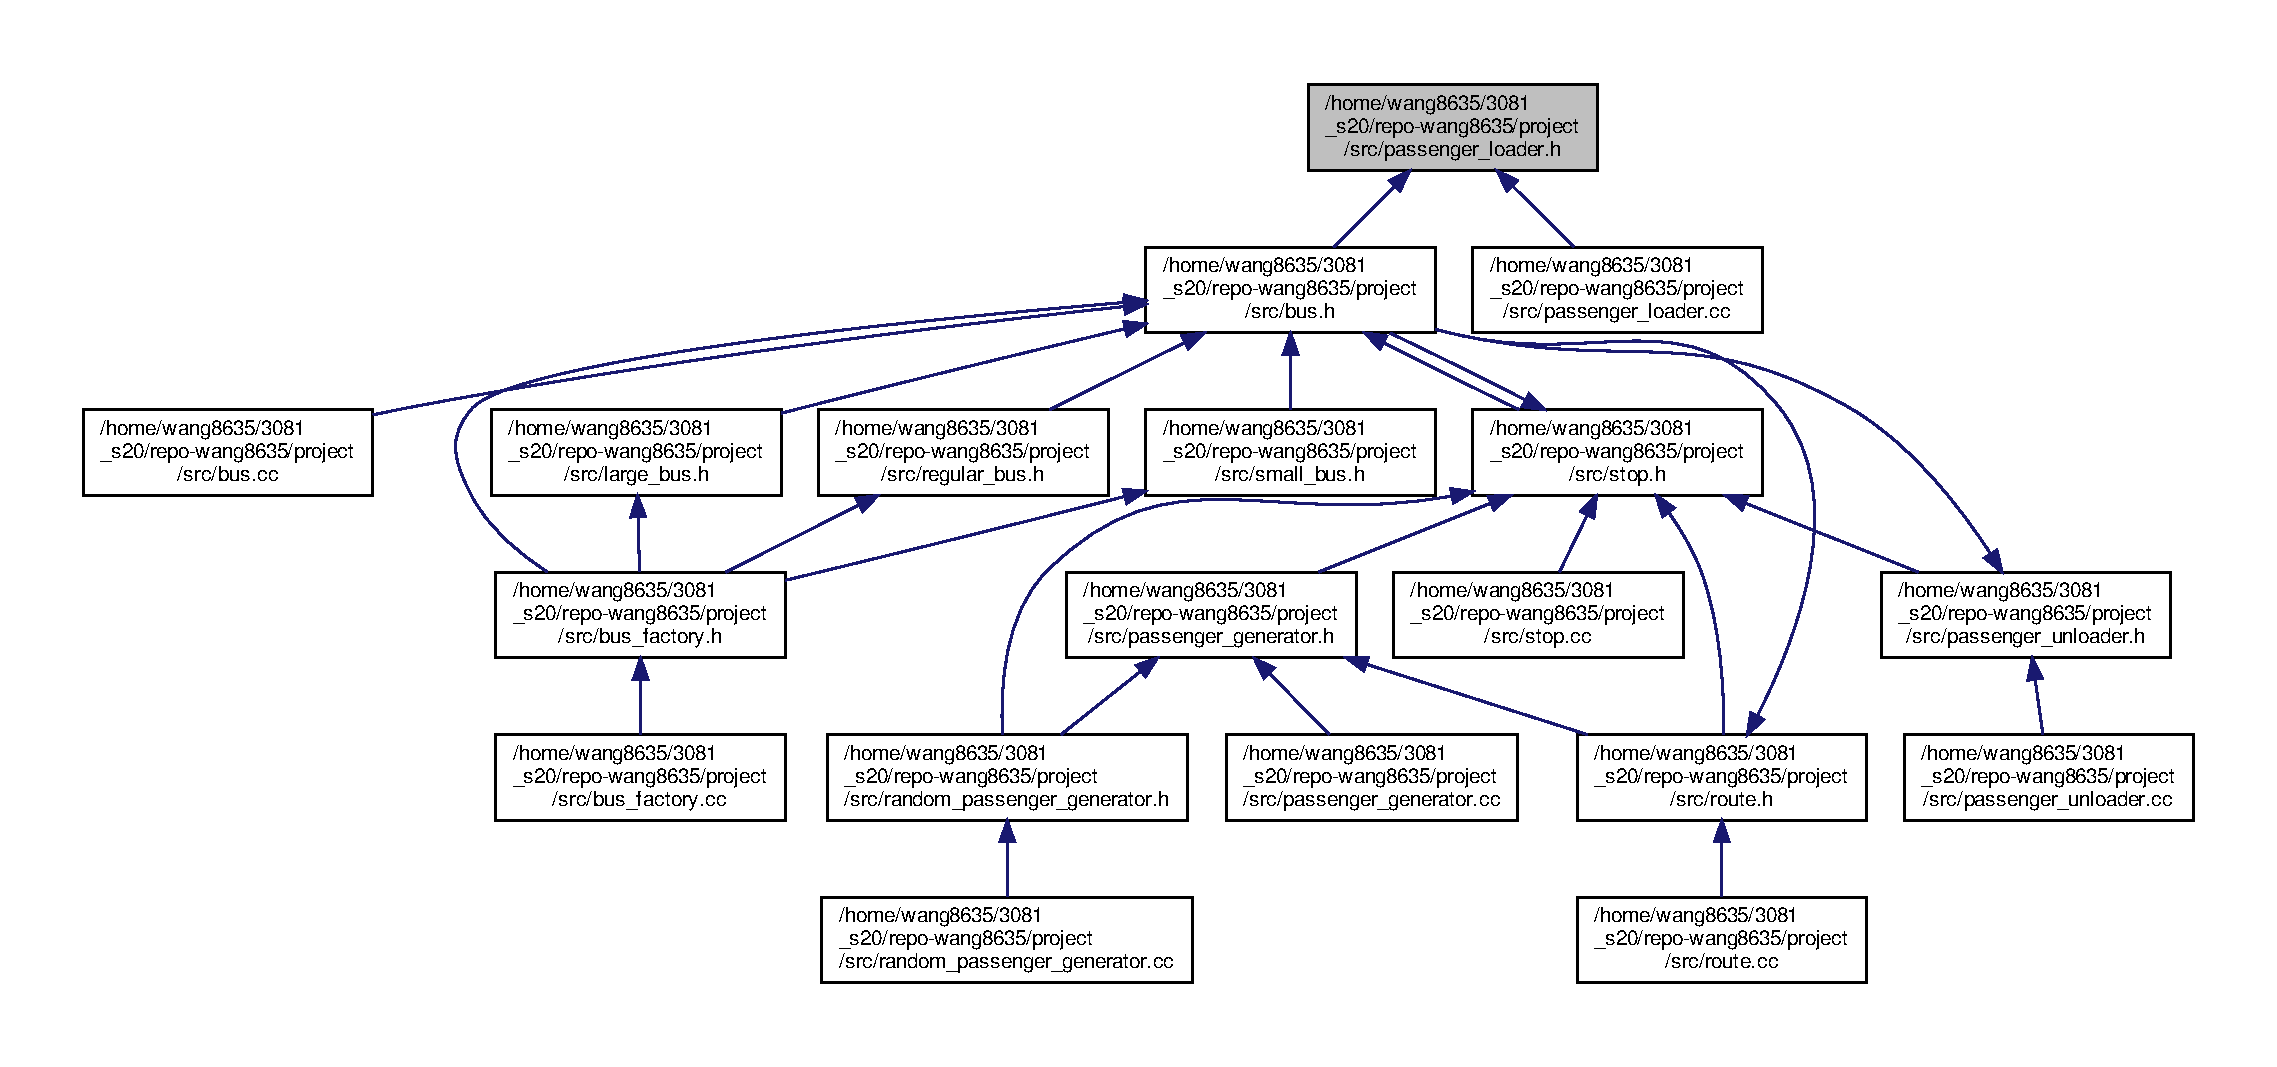
\includegraphics[width=350pt]{passenger__loader_8h__dep__incl}
\end{center}
\end{figure}
\subsection*{Classes}
\begin{DoxyCompactItemize}
\item 
class \hyperlink{classPassengerLoader}{Passenger\+Loader}
\end{DoxyCompactItemize}


\subsection{Detailed Description}
\begin{DoxyCopyright}{Copyright}
2019 3081 Staff, All rights reserved. 
\end{DoxyCopyright}

\hypertarget{passenger__unloader_8cc}{}\section{/home/wang8635/3081\+\_\+s20/repo-\/wang8635/project/src/passenger\+\_\+unloader.cc File Reference}
\label{passenger__unloader_8cc}\index{/home/wang8635/3081\+\_\+s20/repo-\/wang8635/project/src/passenger\+\_\+unloader.\+cc@{/home/wang8635/3081\+\_\+s20/repo-\/wang8635/project/src/passenger\+\_\+unloader.\+cc}}
{\ttfamily \#include \char`\"{}src/passenger\+\_\+unloader.\+h\char`\"{}}\newline
Include dependency graph for passenger\+\_\+unloader.\+cc\+:\nopagebreak
\begin{figure}[H]
\begin{center}
\leavevmode
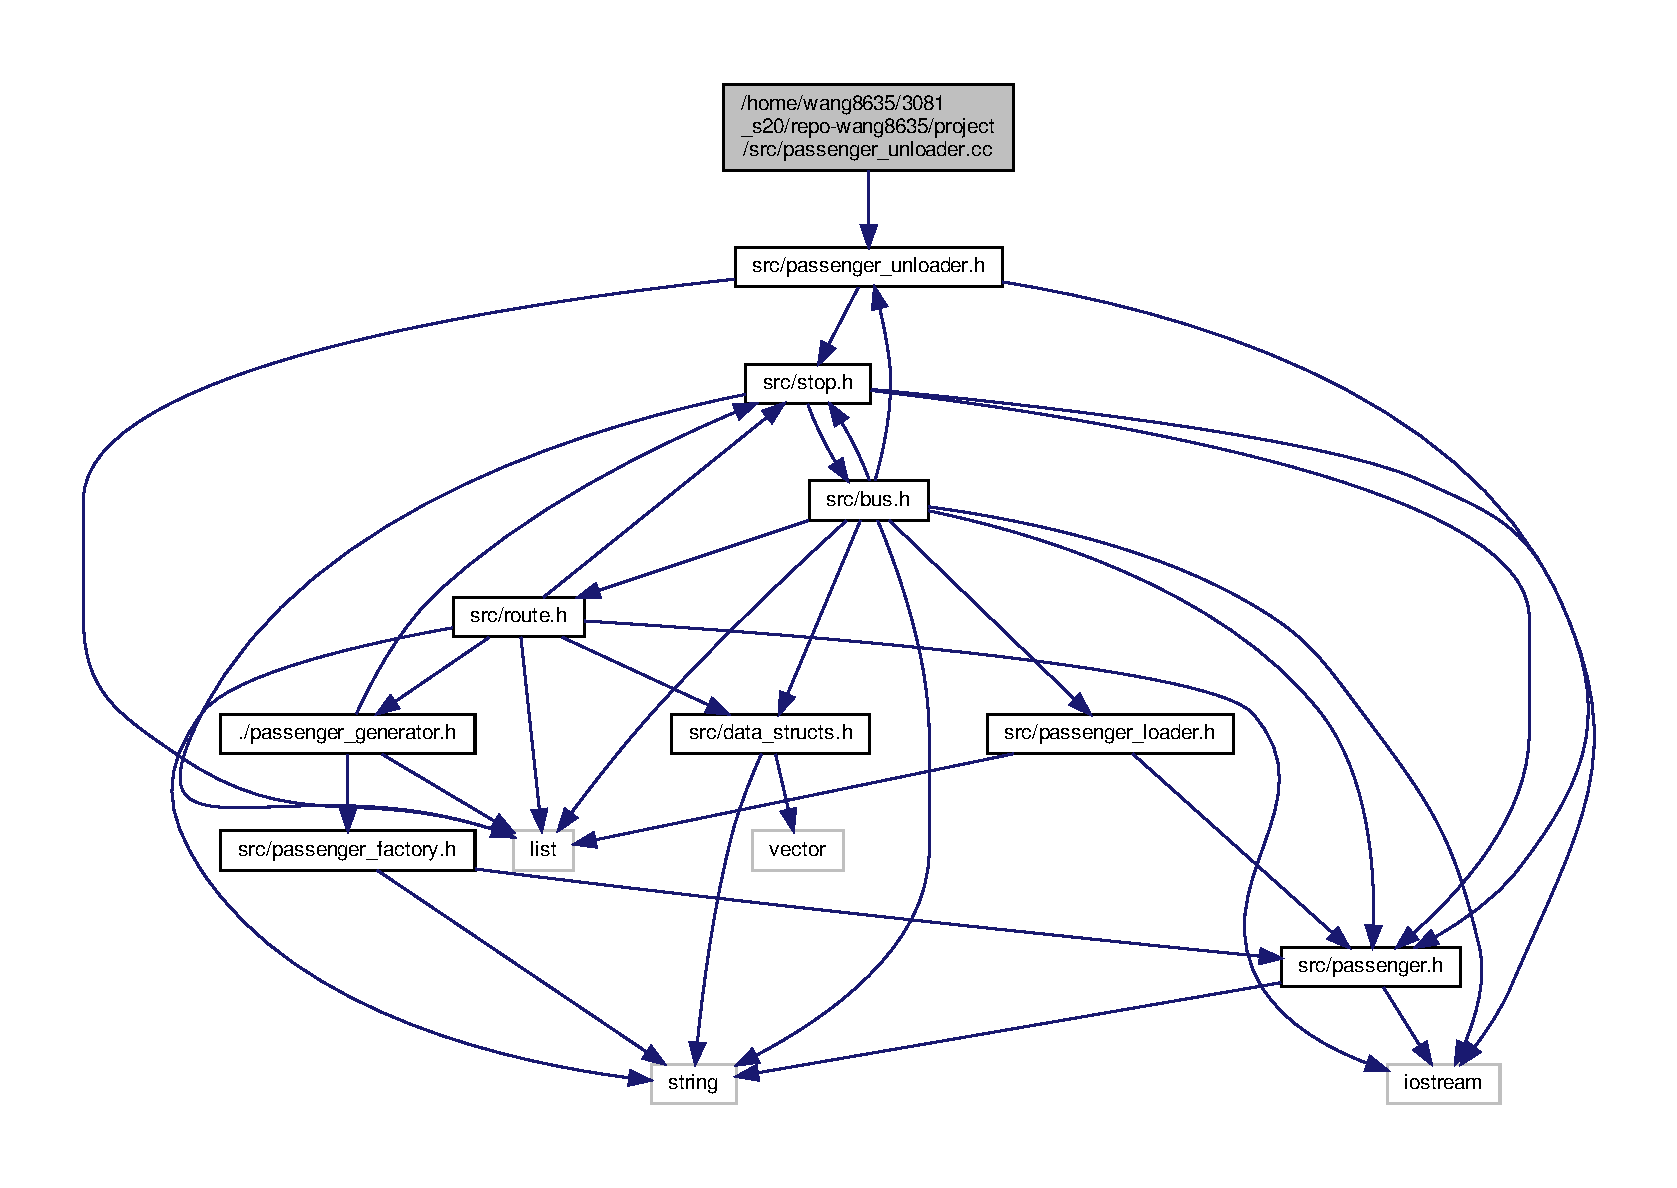
\includegraphics[width=350pt]{passenger__unloader_8cc__incl}
\end{center}
\end{figure}


\subsection{Detailed Description}
\begin{DoxyCopyright}{Copyright}
2019 3081 Staff, All rights reserved. 
\end{DoxyCopyright}

\hypertarget{passenger__unloader_8h}{}\section{/home/wang8635/3081\+\_\+s20/repo-\/wang8635/project/src/passenger\+\_\+unloader.h File Reference}
\label{passenger__unloader_8h}\index{/home/wang8635/3081\+\_\+s20/repo-\/wang8635/project/src/passenger\+\_\+unloader.\+h@{/home/wang8635/3081\+\_\+s20/repo-\/wang8635/project/src/passenger\+\_\+unloader.\+h}}
{\ttfamily \#include $<$list$>$}\newline
{\ttfamily \#include \char`\"{}src/passenger.\+h\char`\"{}}\newline
{\ttfamily \#include \char`\"{}src/stop.\+h\char`\"{}}\newline
Include dependency graph for passenger\+\_\+unloader.\+h\+:
\nopagebreak
\begin{figure}[H]
\begin{center}
\leavevmode
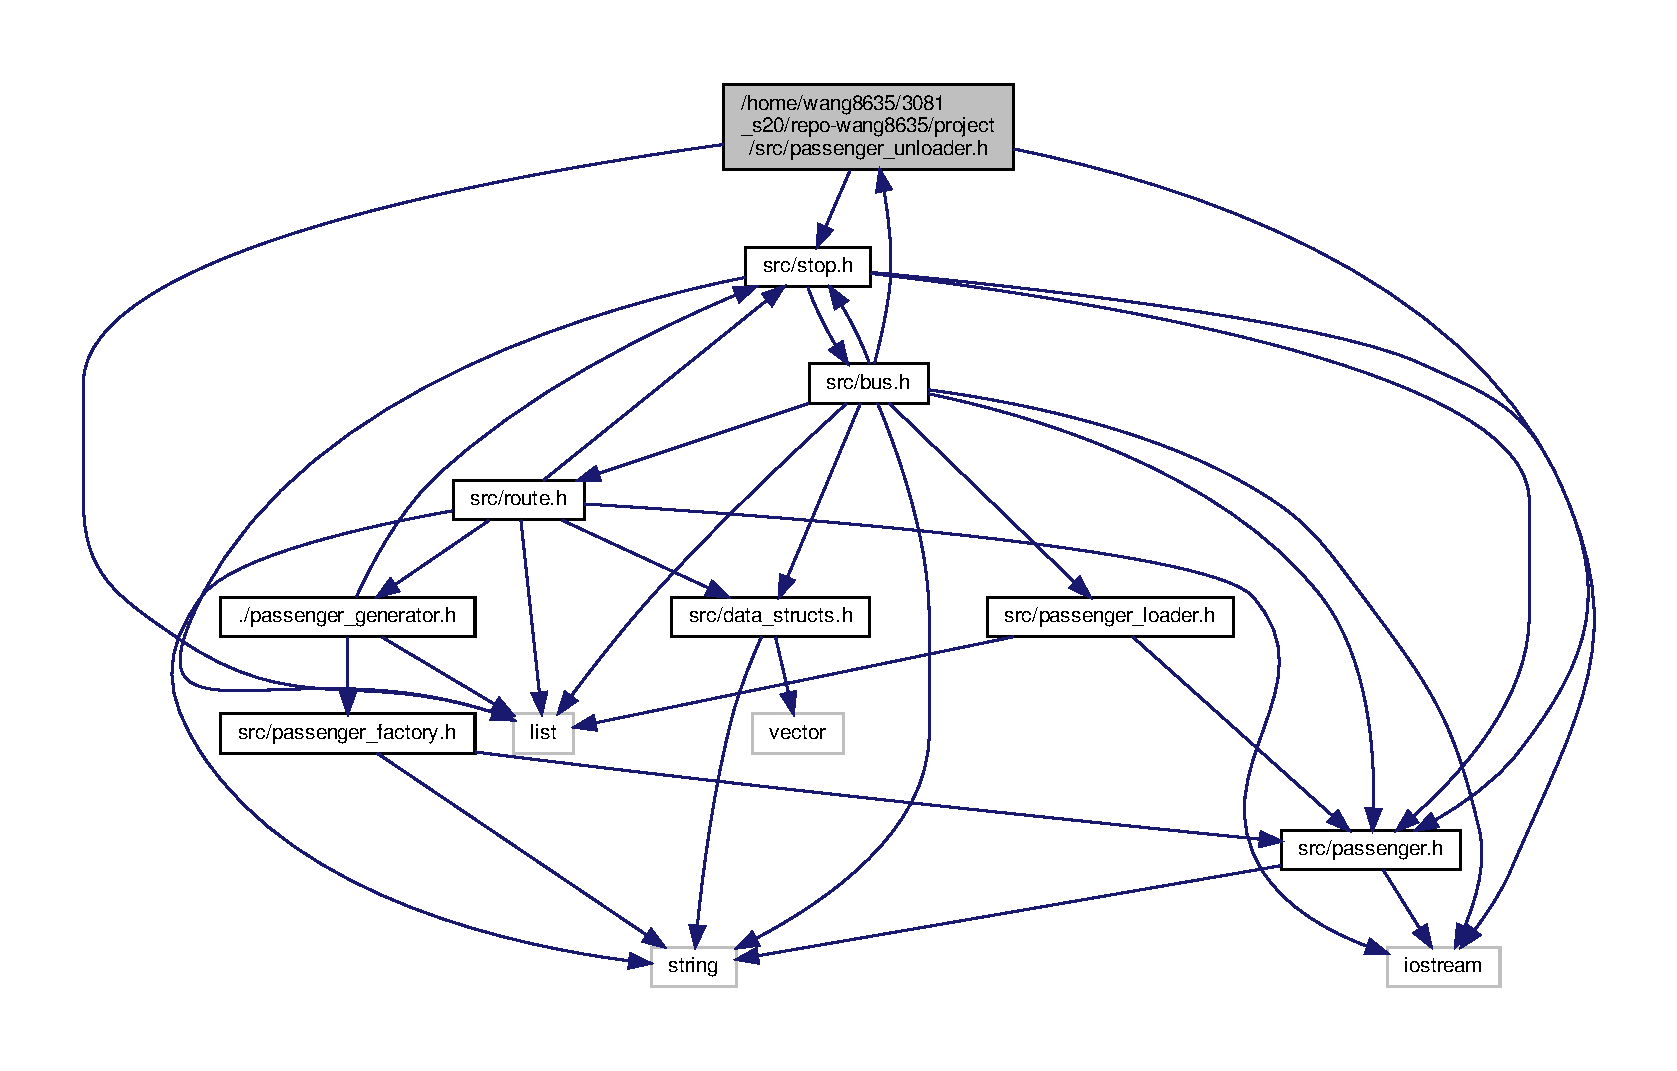
\includegraphics[width=350pt]{passenger__unloader_8h__incl}
\end{center}
\end{figure}
This graph shows which files directly or indirectly include this file\+:
\nopagebreak
\begin{figure}[H]
\begin{center}
\leavevmode
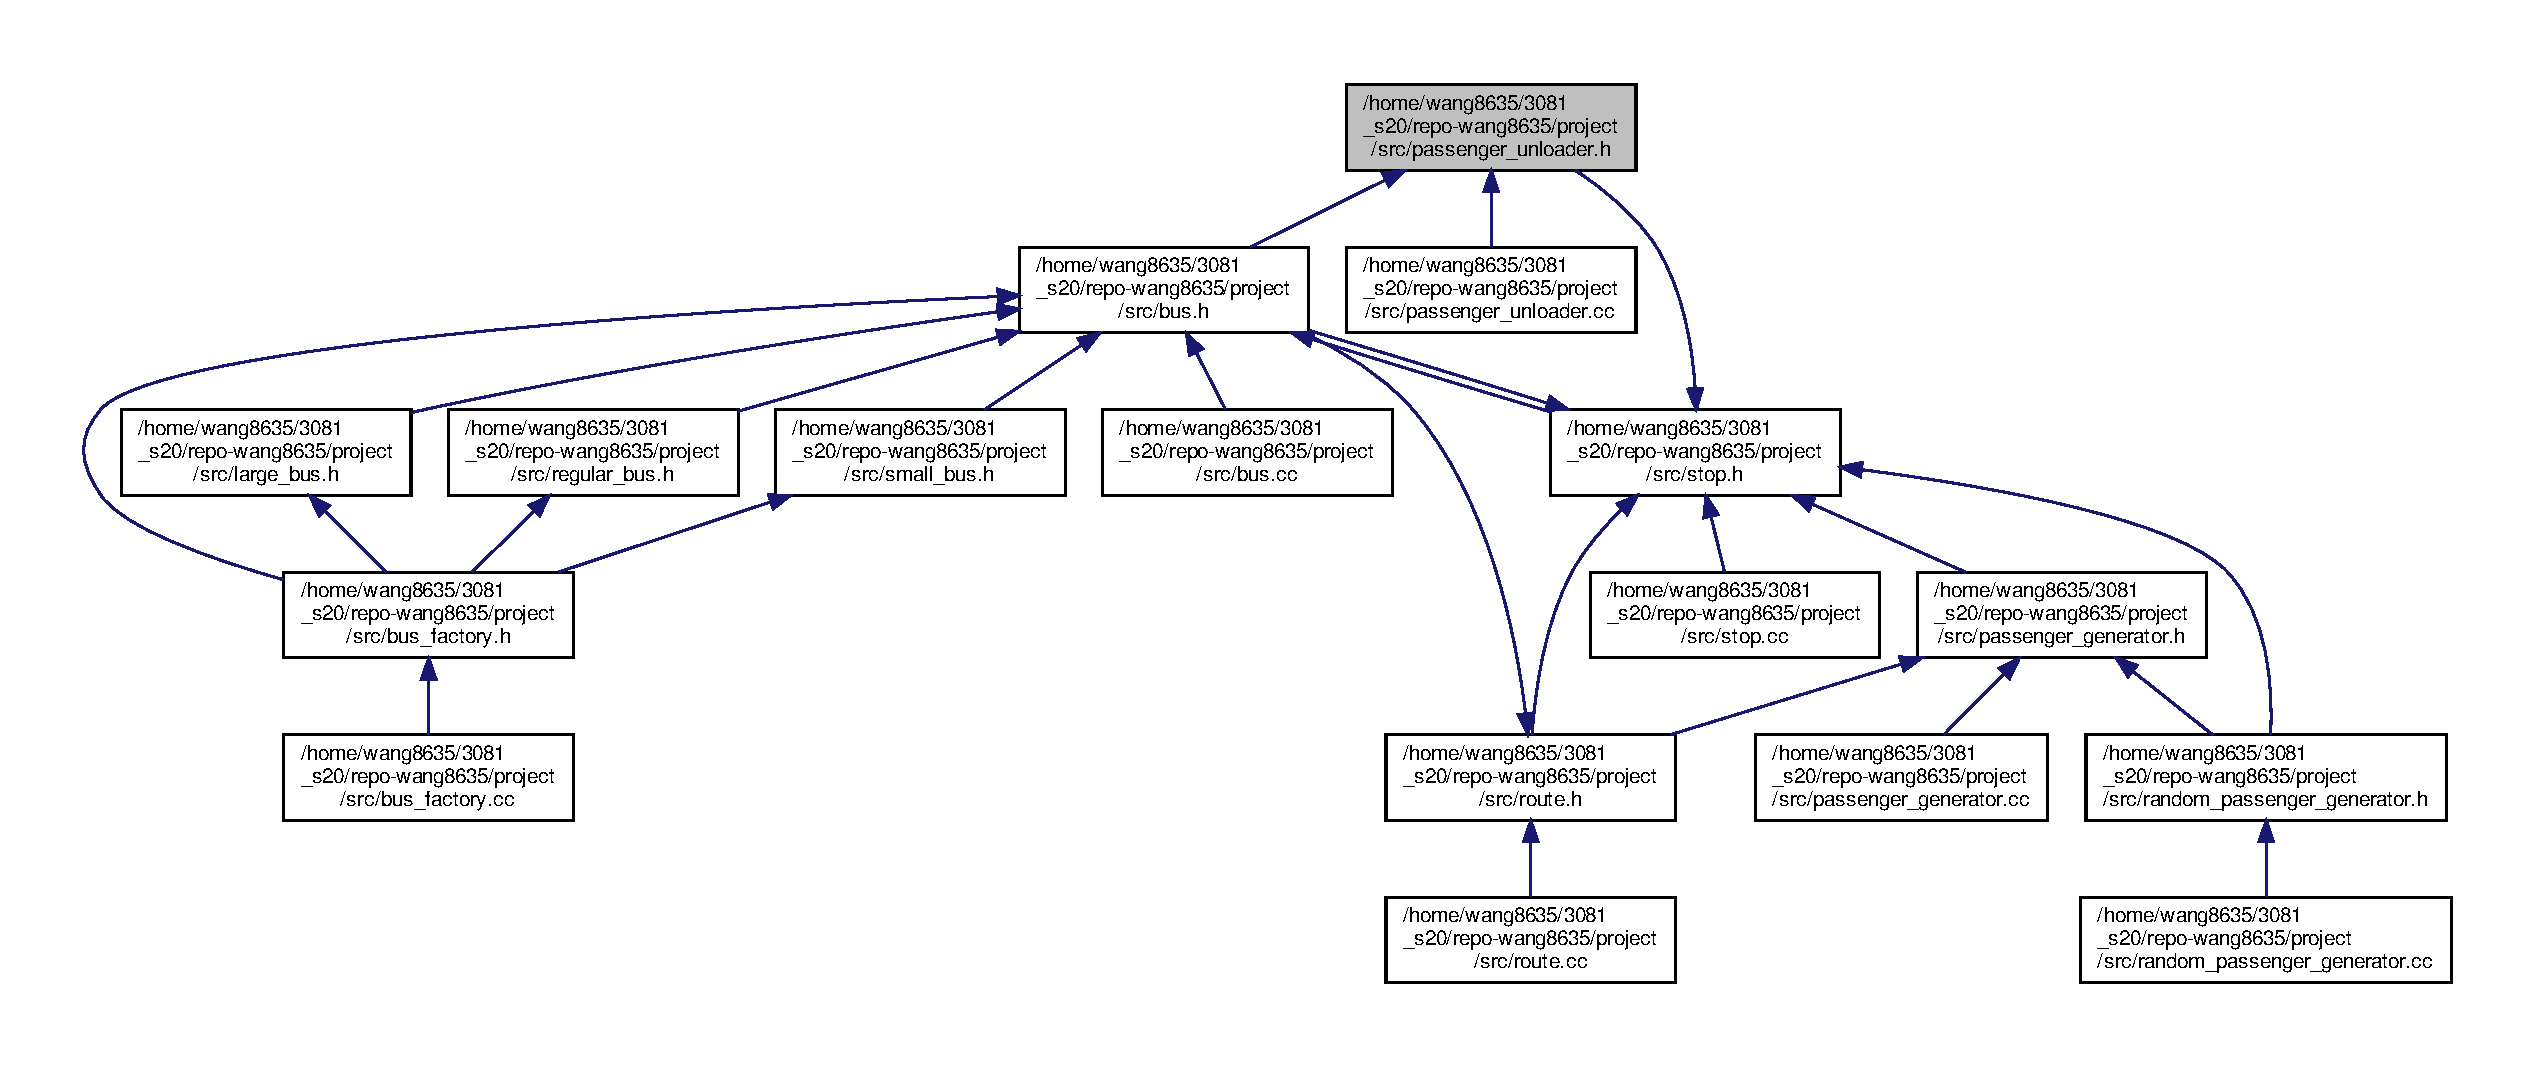
\includegraphics[width=350pt]{passenger__unloader_8h__dep__incl}
\end{center}
\end{figure}
\subsection*{Classes}
\begin{DoxyCompactItemize}
\item 
class \hyperlink{classPassengerUnloader}{Passenger\+Unloader}
\end{DoxyCompactItemize}


\subsection{Detailed Description}
\begin{DoxyCopyright}{Copyright}
2019 3081 Staff, All rights reserved. 
\end{DoxyCopyright}

\hypertarget{random__passenger__generator_8cc}{}\section{/home/wang8635/3081\+\_\+s20/repo-\/wang8635/project/src/random\+\_\+passenger\+\_\+generator.cc File Reference}
\label{random__passenger__generator_8cc}\index{/home/wang8635/3081\+\_\+s20/repo-\/wang8635/project/src/random\+\_\+passenger\+\_\+generator.\+cc@{/home/wang8635/3081\+\_\+s20/repo-\/wang8635/project/src/random\+\_\+passenger\+\_\+generator.\+cc}}
{\ttfamily \#include \char`\"{}src/random\+\_\+passenger\+\_\+generator.\+h\char`\"{}}\newline
Include dependency graph for random\+\_\+passenger\+\_\+generator.\+cc\+:\nopagebreak
\begin{figure}[H]
\begin{center}
\leavevmode
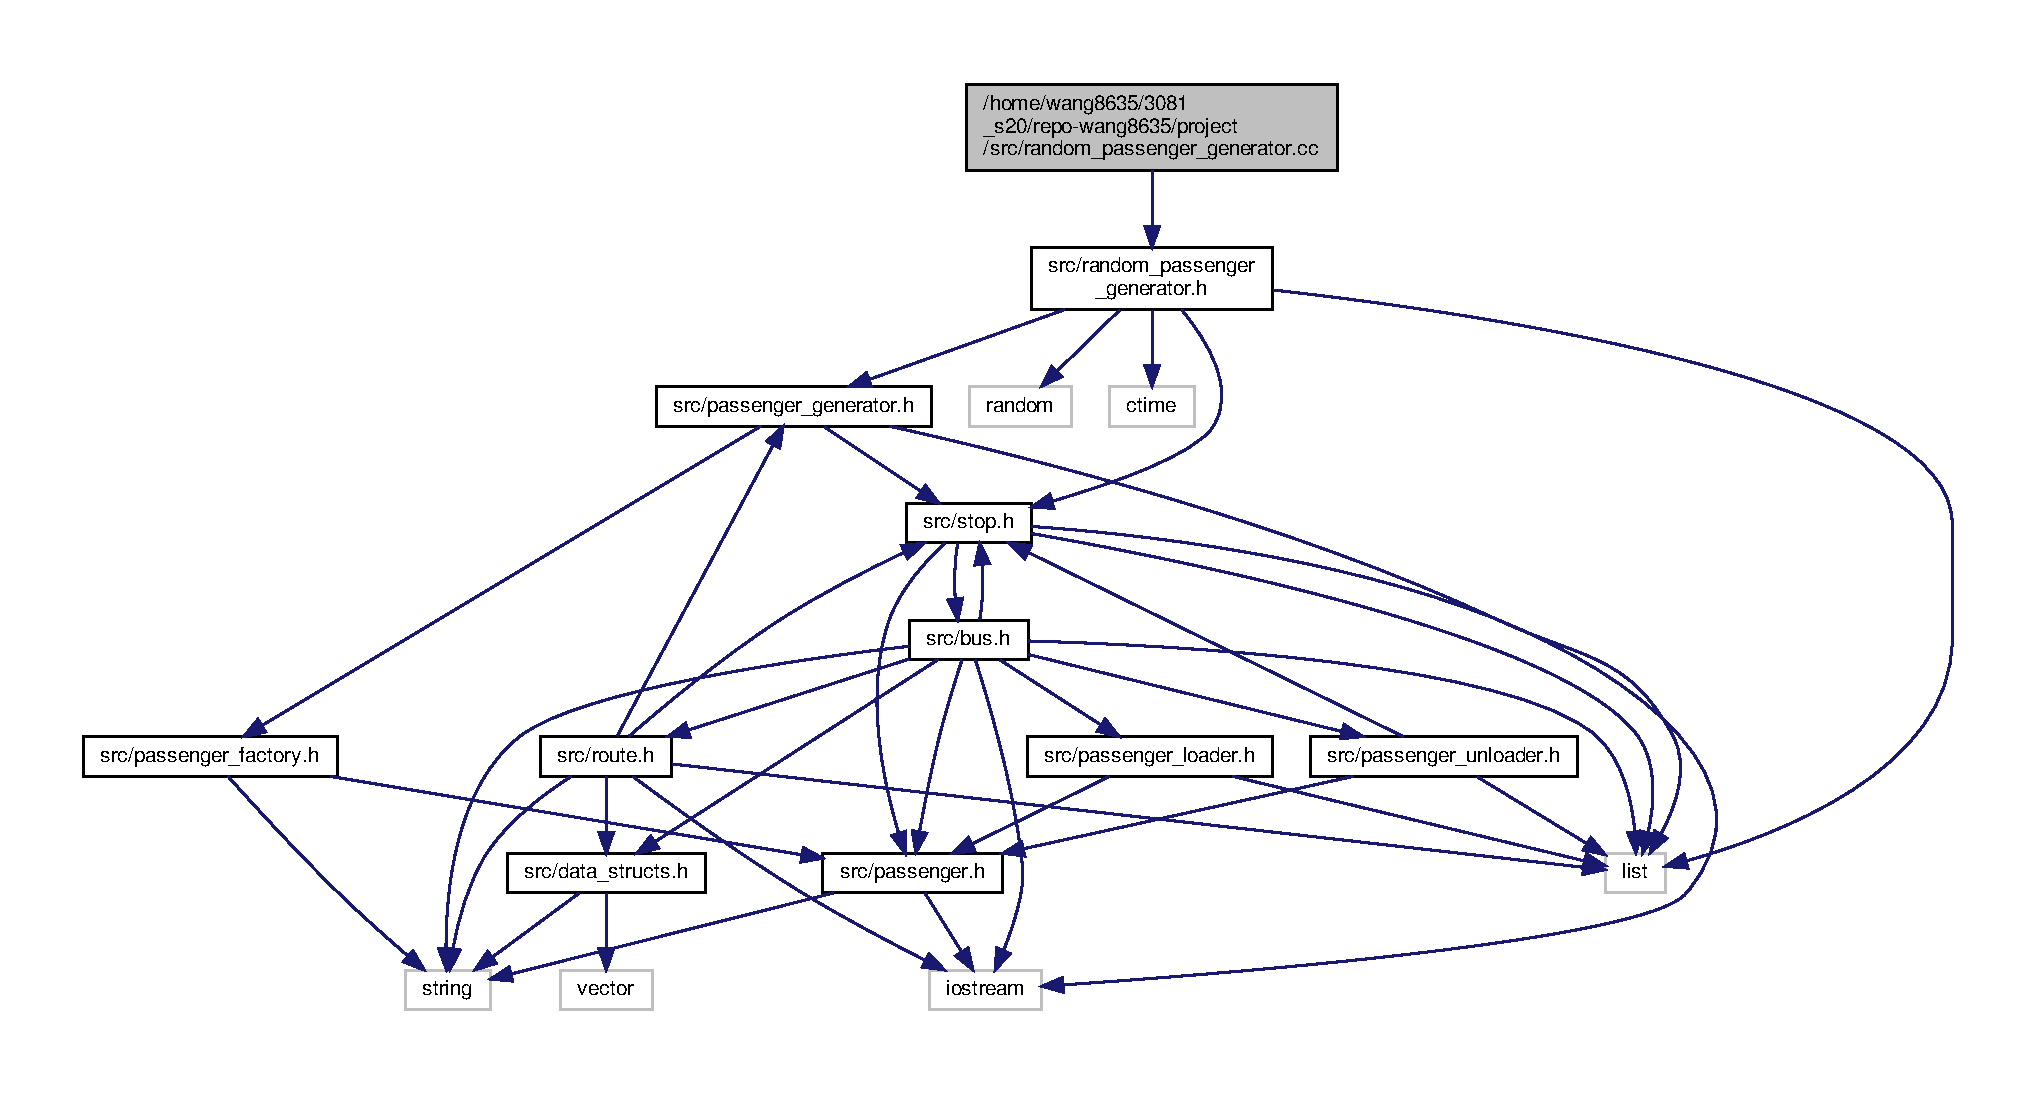
\includegraphics[width=350pt]{random__passenger__generator_8cc__incl}
\end{center}
\end{figure}


\subsection{Detailed Description}
\begin{DoxyCopyright}{Copyright}
2019 3081 Staff, All rights reserved. 
\end{DoxyCopyright}

\hypertarget{random__passenger__generator_8h}{}\section{/home/wang8635/3081\+\_\+s20/repo-\/wang8635/project/src/random\+\_\+passenger\+\_\+generator.h File Reference}
\label{random__passenger__generator_8h}\index{/home/wang8635/3081\+\_\+s20/repo-\/wang8635/project/src/random\+\_\+passenger\+\_\+generator.\+h@{/home/wang8635/3081\+\_\+s20/repo-\/wang8635/project/src/random\+\_\+passenger\+\_\+generator.\+h}}
{\ttfamily \#include $<$list$>$}\newline
{\ttfamily \#include $<$random$>$}\newline
{\ttfamily \#include $<$ctime$>$}\newline
{\ttfamily \#include \char`\"{}src/passenger\+\_\+generator.\+h\char`\"{}}\newline
{\ttfamily \#include \char`\"{}src/stop.\+h\char`\"{}}\newline
Include dependency graph for random\+\_\+passenger\+\_\+generator.\+h\+:\nopagebreak
\begin{figure}[H]
\begin{center}
\leavevmode
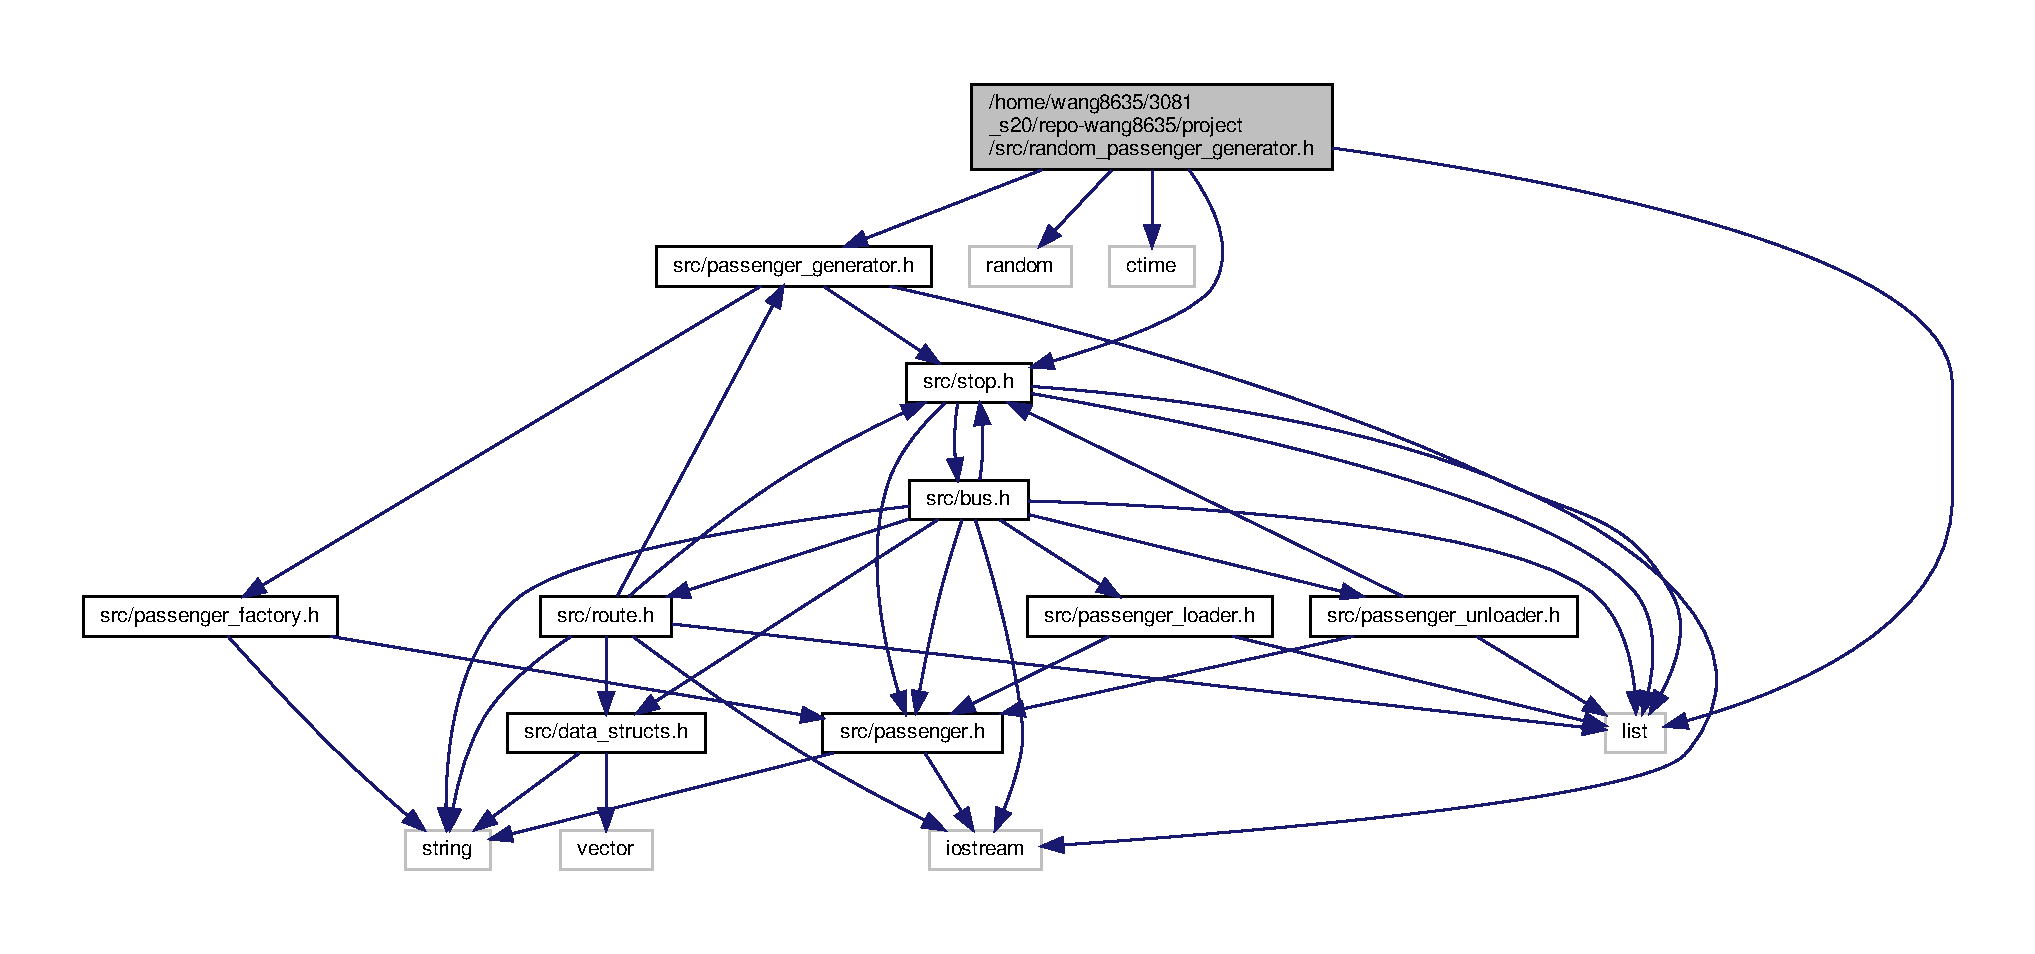
\includegraphics[width=350pt]{random__passenger__generator_8h__incl}
\end{center}
\end{figure}
This graph shows which files directly or indirectly include this file\+:\nopagebreak
\begin{figure}[H]
\begin{center}
\leavevmode
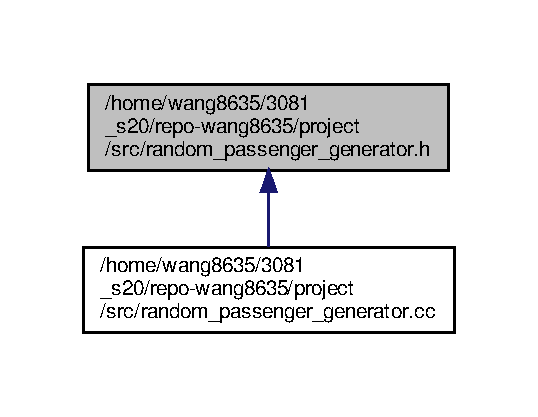
\includegraphics[width=258pt]{random__passenger__generator_8h__dep__incl}
\end{center}
\end{figure}
\subsection*{Classes}
\begin{DoxyCompactItemize}
\item 
class \hyperlink{classRandomPassengerGenerator}{Random\+Passenger\+Generator}
\end{DoxyCompactItemize}


\subsection{Detailed Description}
\begin{DoxyCopyright}{Copyright}
2019 3081 Staff, All rights reserved. 
\end{DoxyCopyright}

\hypertarget{route_8cc}{}\section{/home/wang8635/3081\+\_\+s20/repo-\/wang8635/project/src/route.cc File Reference}
\label{route_8cc}\index{/home/wang8635/3081\+\_\+s20/repo-\/wang8635/project/src/route.\+cc@{/home/wang8635/3081\+\_\+s20/repo-\/wang8635/project/src/route.\+cc}}
{\ttfamily \#include $<$vector$>$}\newline
{\ttfamily \#include \char`\"{}src/route.\+h\char`\"{}}\newline
Include dependency graph for route.\+cc\+:\nopagebreak
\begin{figure}[H]
\begin{center}
\leavevmode
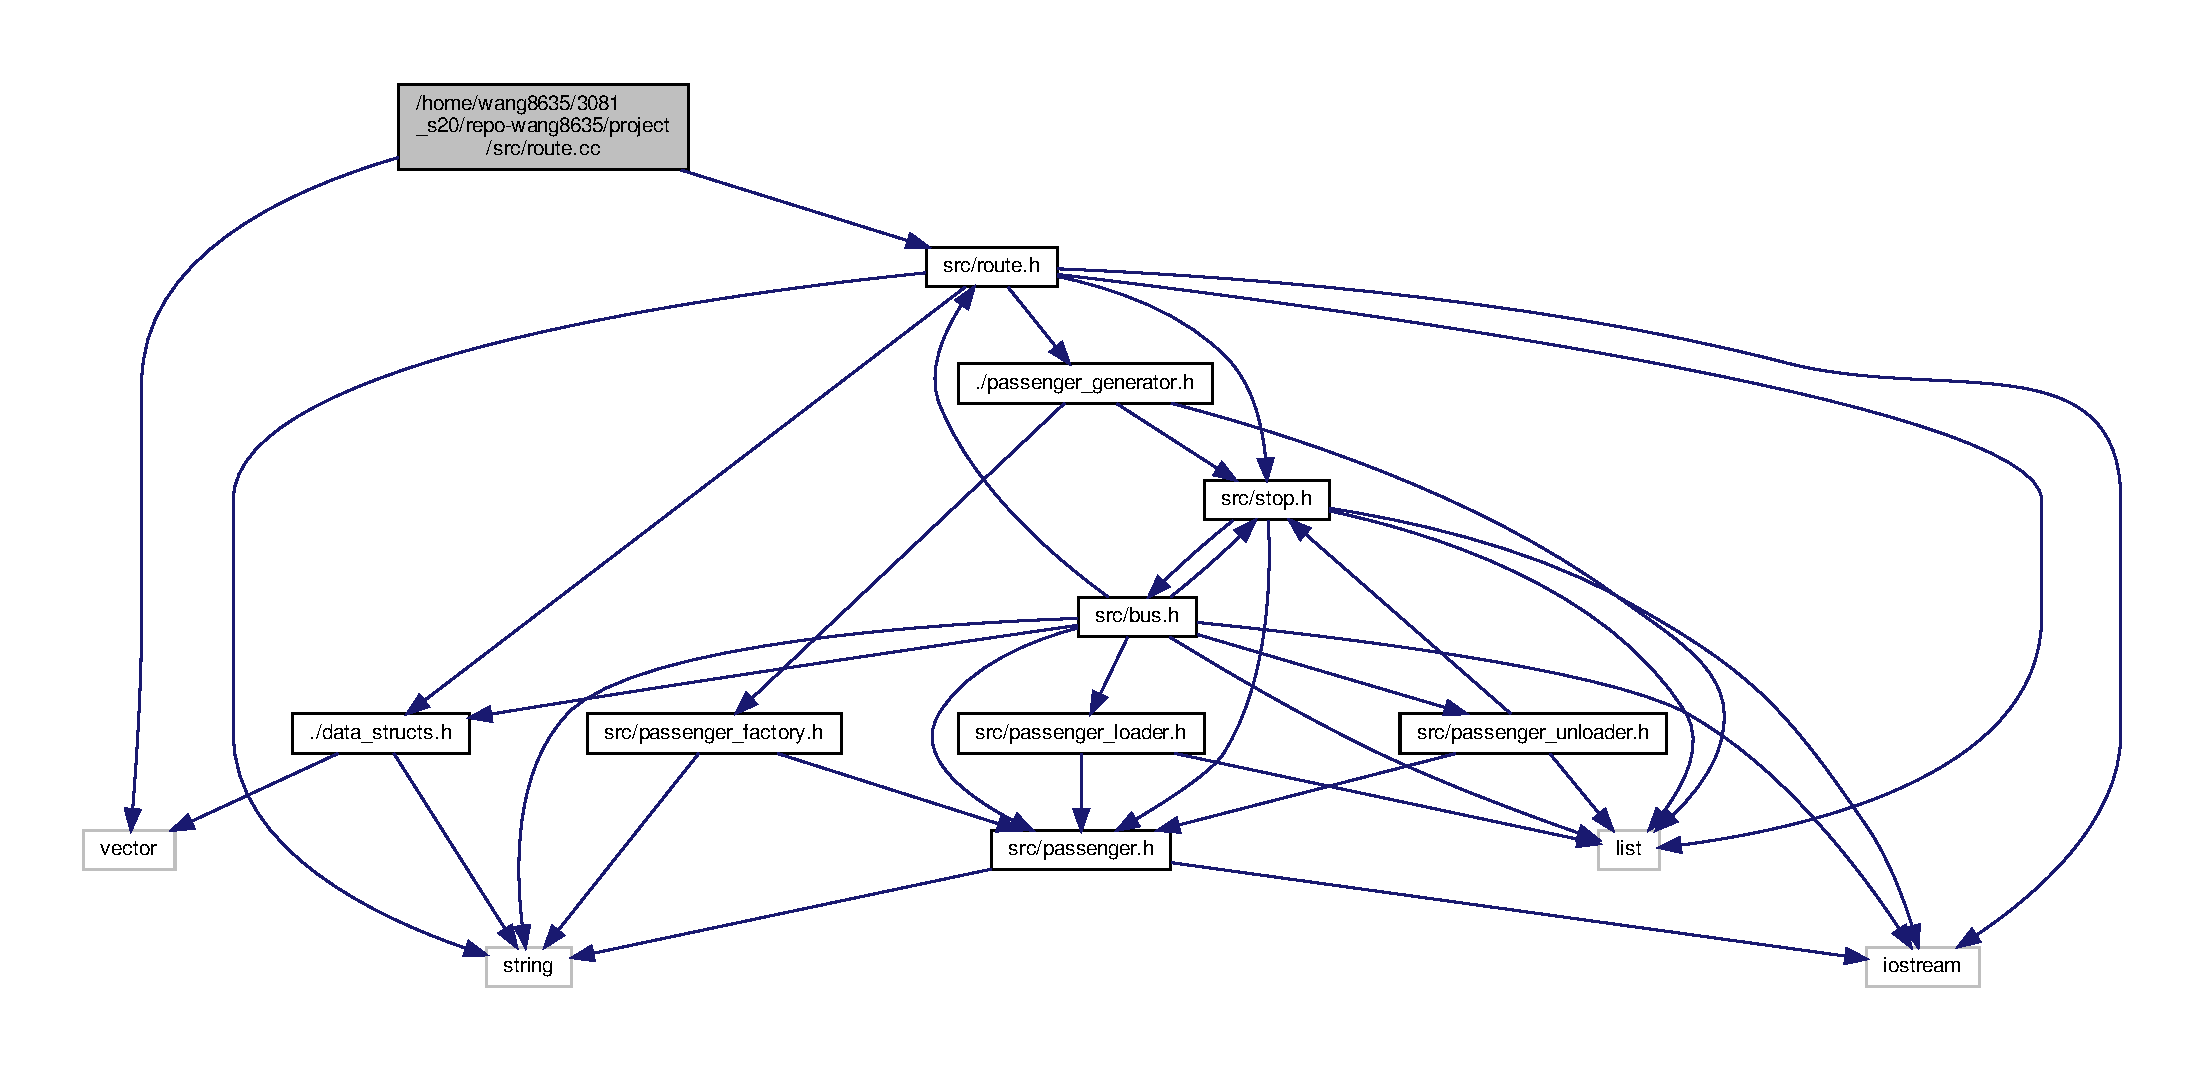
\includegraphics[width=350pt]{route_8cc__incl}
\end{center}
\end{figure}


\subsection{Detailed Description}
\begin{DoxyCopyright}{Copyright}
2019 3081 Staff, All rights reserved. 
\end{DoxyCopyright}

\hypertarget{route_8h}{}\section{/home/wang8635/3081\+\_\+s20/repo-\/wang8635/project/src/route.h File Reference}
\label{route_8h}\index{/home/wang8635/3081\+\_\+s20/repo-\/wang8635/project/src/route.\+h@{/home/wang8635/3081\+\_\+s20/repo-\/wang8635/project/src/route.\+h}}
{\ttfamily \#include $<$list$>$}\newline
{\ttfamily \#include $<$iostream$>$}\newline
{\ttfamily \#include $<$string$>$}\newline
{\ttfamily \#include \char`\"{}./data\+\_\+structs.\+h\char`\"{}}\newline
{\ttfamily \#include \char`\"{}./passenger\+\_\+generator.\+h\char`\"{}}\newline
{\ttfamily \#include \char`\"{}./stop.\+h\char`\"{}}\newline
Include dependency graph for route.\+h\+:
\nopagebreak
\begin{figure}[H]
\begin{center}
\leavevmode
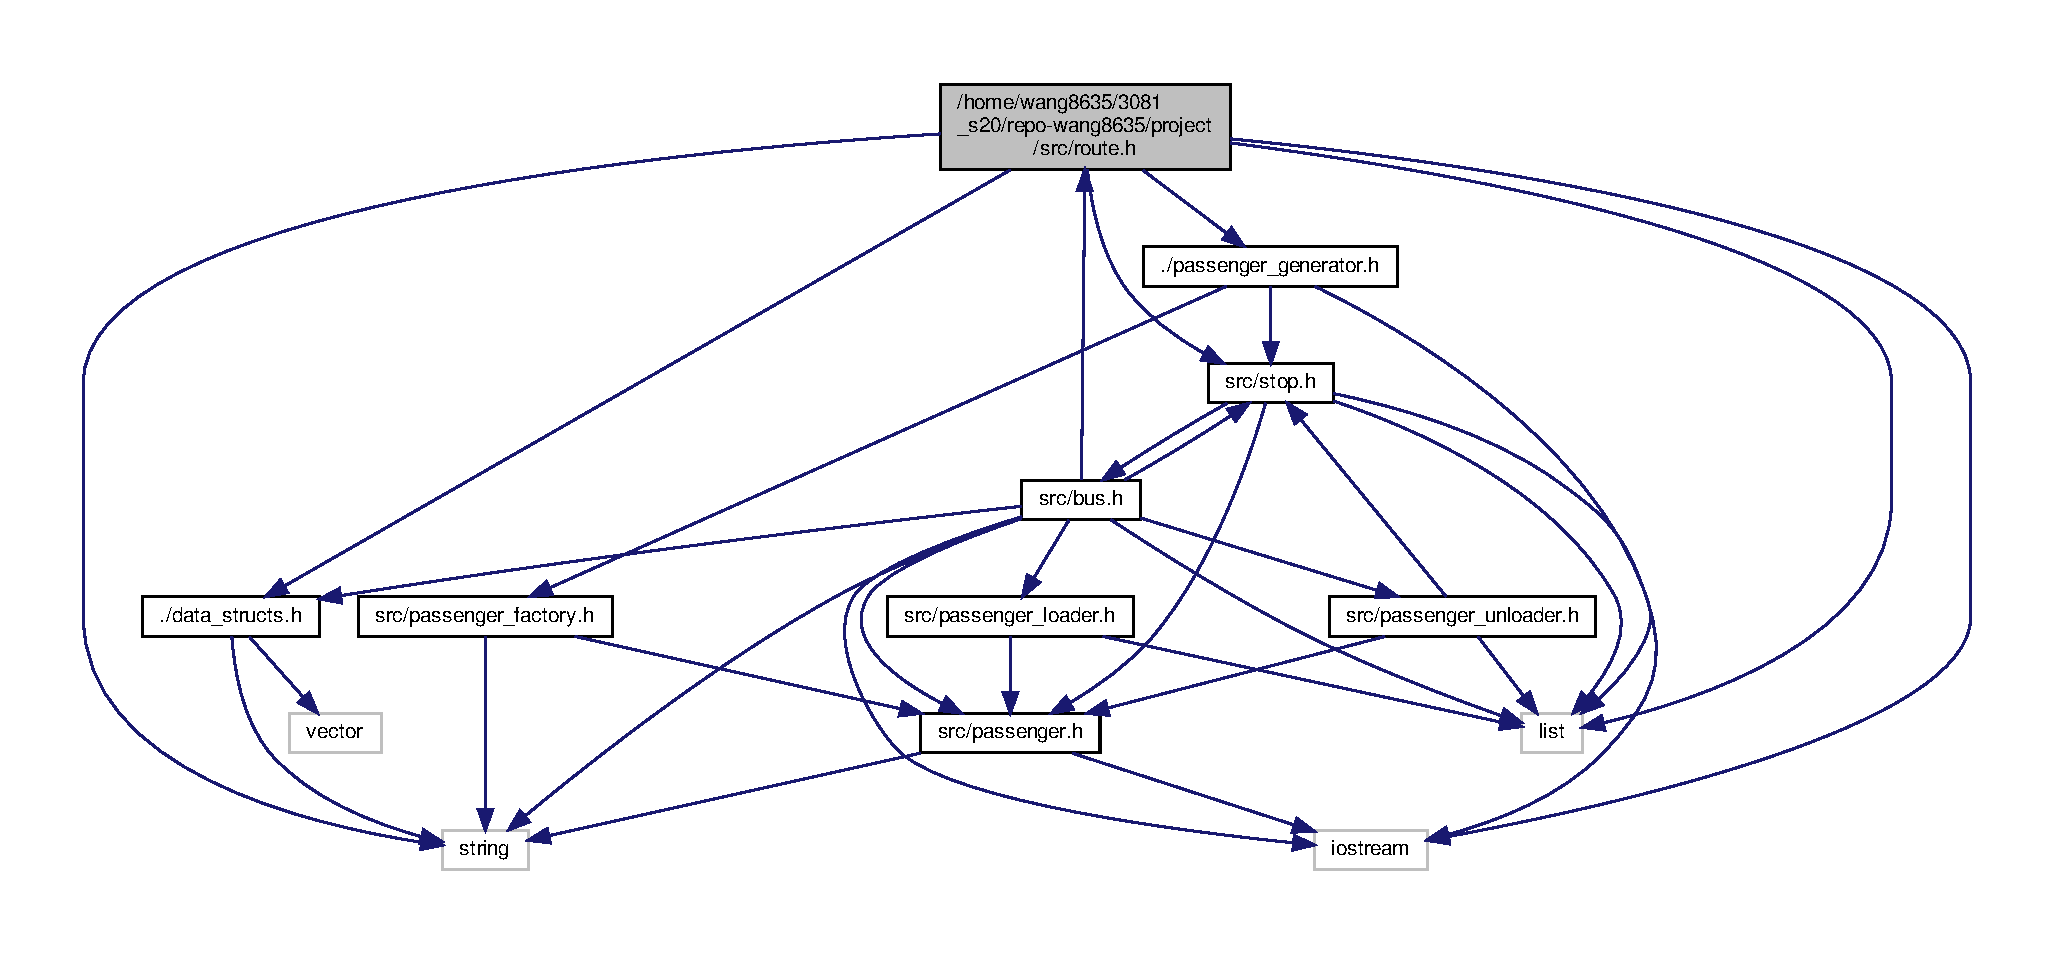
\includegraphics[width=350pt]{route_8h__incl}
\end{center}
\end{figure}
This graph shows which files directly or indirectly include this file\+:
\nopagebreak
\begin{figure}[H]
\begin{center}
\leavevmode
\includegraphics[width=350pt]{route_8h__dep__incl}
\end{center}
\end{figure}
\subsection*{Classes}
\begin{DoxyCompactItemize}
\item 
class \hyperlink{classRoute}{Route}
\end{DoxyCompactItemize}


\subsection{Detailed Description}
2019 3081 Staff, All rights reserved. 
\hypertarget{stop_8cc}{}\section{/home/wang8635/3081\+\_\+s20/repo-\/wang8635/project/src/stop.cc File Reference}
\label{stop_8cc}\index{/home/wang8635/3081\+\_\+s20/repo-\/wang8635/project/src/stop.\+cc@{/home/wang8635/3081\+\_\+s20/repo-\/wang8635/project/src/stop.\+cc}}
{\ttfamily \#include $<$iostream$>$}\newline
{\ttfamily \#include $<$vector$>$}\newline
{\ttfamily \#include \char`\"{}src/stop.\+h\char`\"{}}\newline
Include dependency graph for stop.\+cc\+:\nopagebreak
\begin{figure}[H]
\begin{center}
\leavevmode
\includegraphics[width=350pt]{stop_8cc__incl}
\end{center}
\end{figure}


\subsection{Detailed Description}
\begin{DoxyCopyright}{Copyright}
2019 3081 Staff, All rights reserved. 
\end{DoxyCopyright}

%--- End generated contents ---

% Index
\backmatter
\newpage
\phantomsection
\clearemptydoublepage
\addcontentsline{toc}{chapter}{Index}
\printindex

\end{document}
